\newpage
%Punto 2
\section{Technical Specification}
  %Punto 2.1
  \subsection{Cable Jacket}
  \begin{figure}
    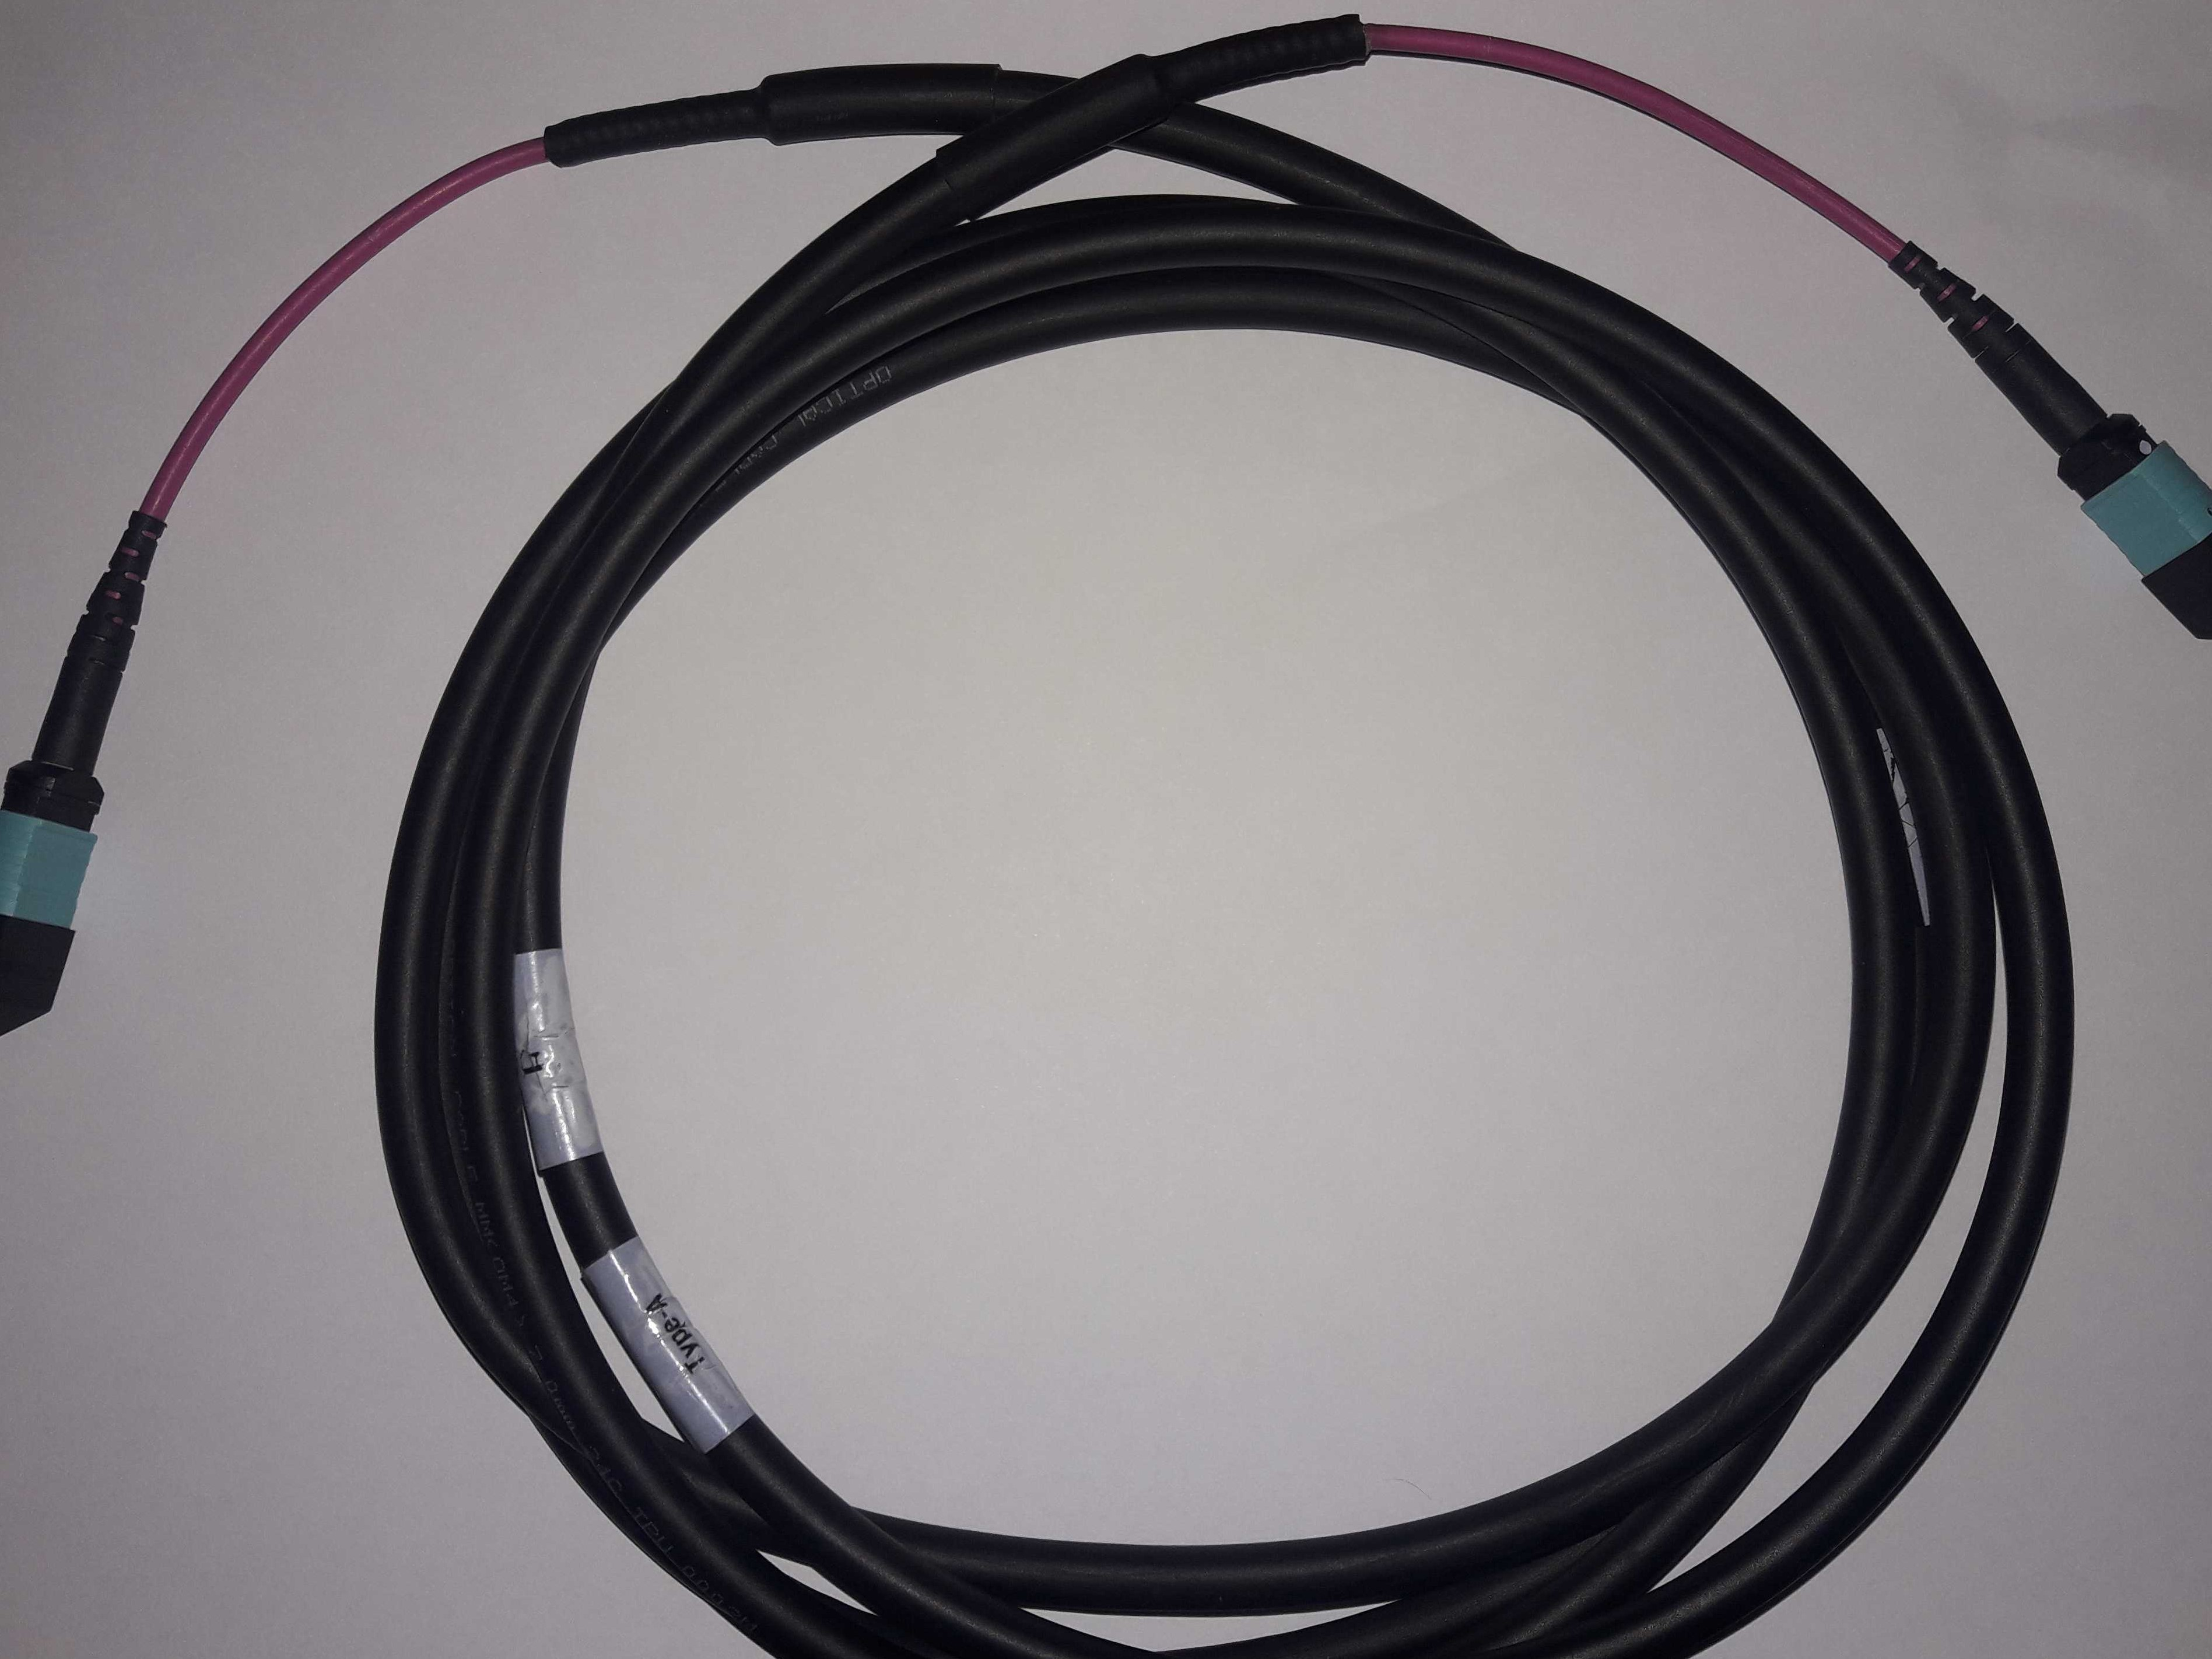
\includegraphics[width=11cm]{images/mtp_militar_cable.jpg}
    \centering
    \caption*{Prototype of the Armored Cable}
  \end{figure}
  This armored cable has the following features.
  \begin{itemize}
    \item Strong tensile strength.
    \item Strong resistance to pressure.
    \item Flexible and resistant to any type of bending.
    \item Resistant to oil, wear, and fire.
  \end{itemize}
\newpage

\vspace{10 mm}
  Additional Technical Specifications:
  \begin{figure}
    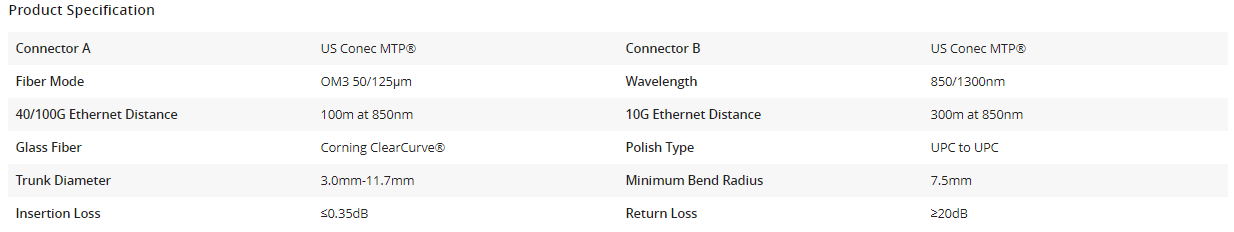
\includegraphics[width=\textwidth]{images/2.png}
    \caption*{MTP/MPO Connectors}
  \end{figure}

\newpage
  %Punto 2.2
  \subsection{MTP/MPO Connectors}
  MTP/MPO main characteristics and features
  %Punto 2.2.1
  \subsubsection{MTP/MPO Connector}
  Each cable contains 24 filaments with 1 MTP/MPO connector at each end.
  \begin{figure}
    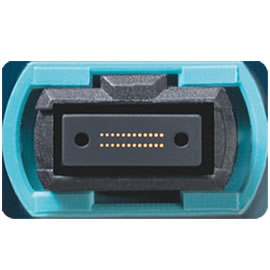
\includegraphics[width=5cm]{images/3.jpg}
    \centering
    \caption{MTP/MPO Connectors}
  \end{figure}

\newpage
  %Punto 2.3
  \subsection{MTP/MPO Adapters}
  Each connection between cables has to use a key-up and key-down adapter in order to work and function properly.
  \begin{figure}
    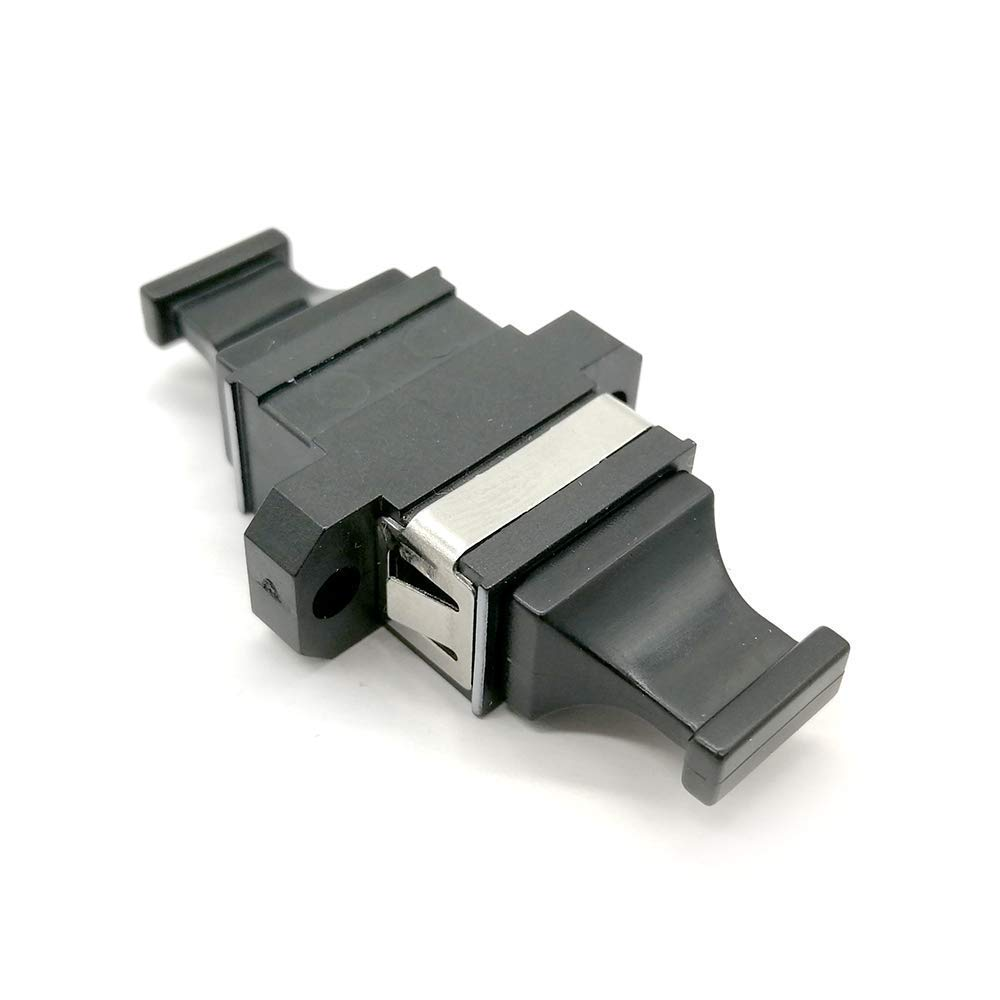
\includegraphics[width=6cm]{images/4.jpg}
    \centering
    \caption{Key-up and Key-down adapter}
  \end{figure}

\newpage
  %Punto 2.4
  \subsection{The MTP / MPO Female and Male Connectors}
  The MTP/MPO cables always connect to another MTP/MPO cable, each connector has a connection type which is either Female or Male.
  \begin{figure}
    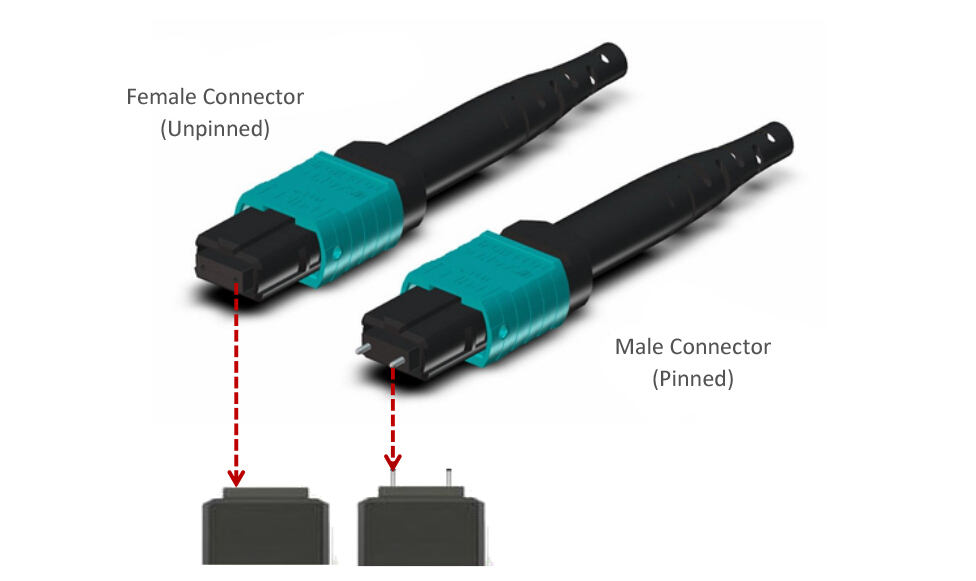
\includegraphics[width=\textwidth]{images/5.jpeg}
    \caption{MTP/MPO Connectors Female/Male}
  \end{figure}

\newpage
  %Punto 2.5
  \subsection{Cable Polarity}
  The cable can be purchased in 3 polarity modes, these are:
  \begin{itemize}
    \item Type A
    \item Type B
    \item Type C
  \end{itemize}
  For documentation purposes, we will turn our focus on Polarity Type-A cables.
  \begin{figure}
    \centering
    \begin{subfigure}{0.48\textwidth}
      \centering
      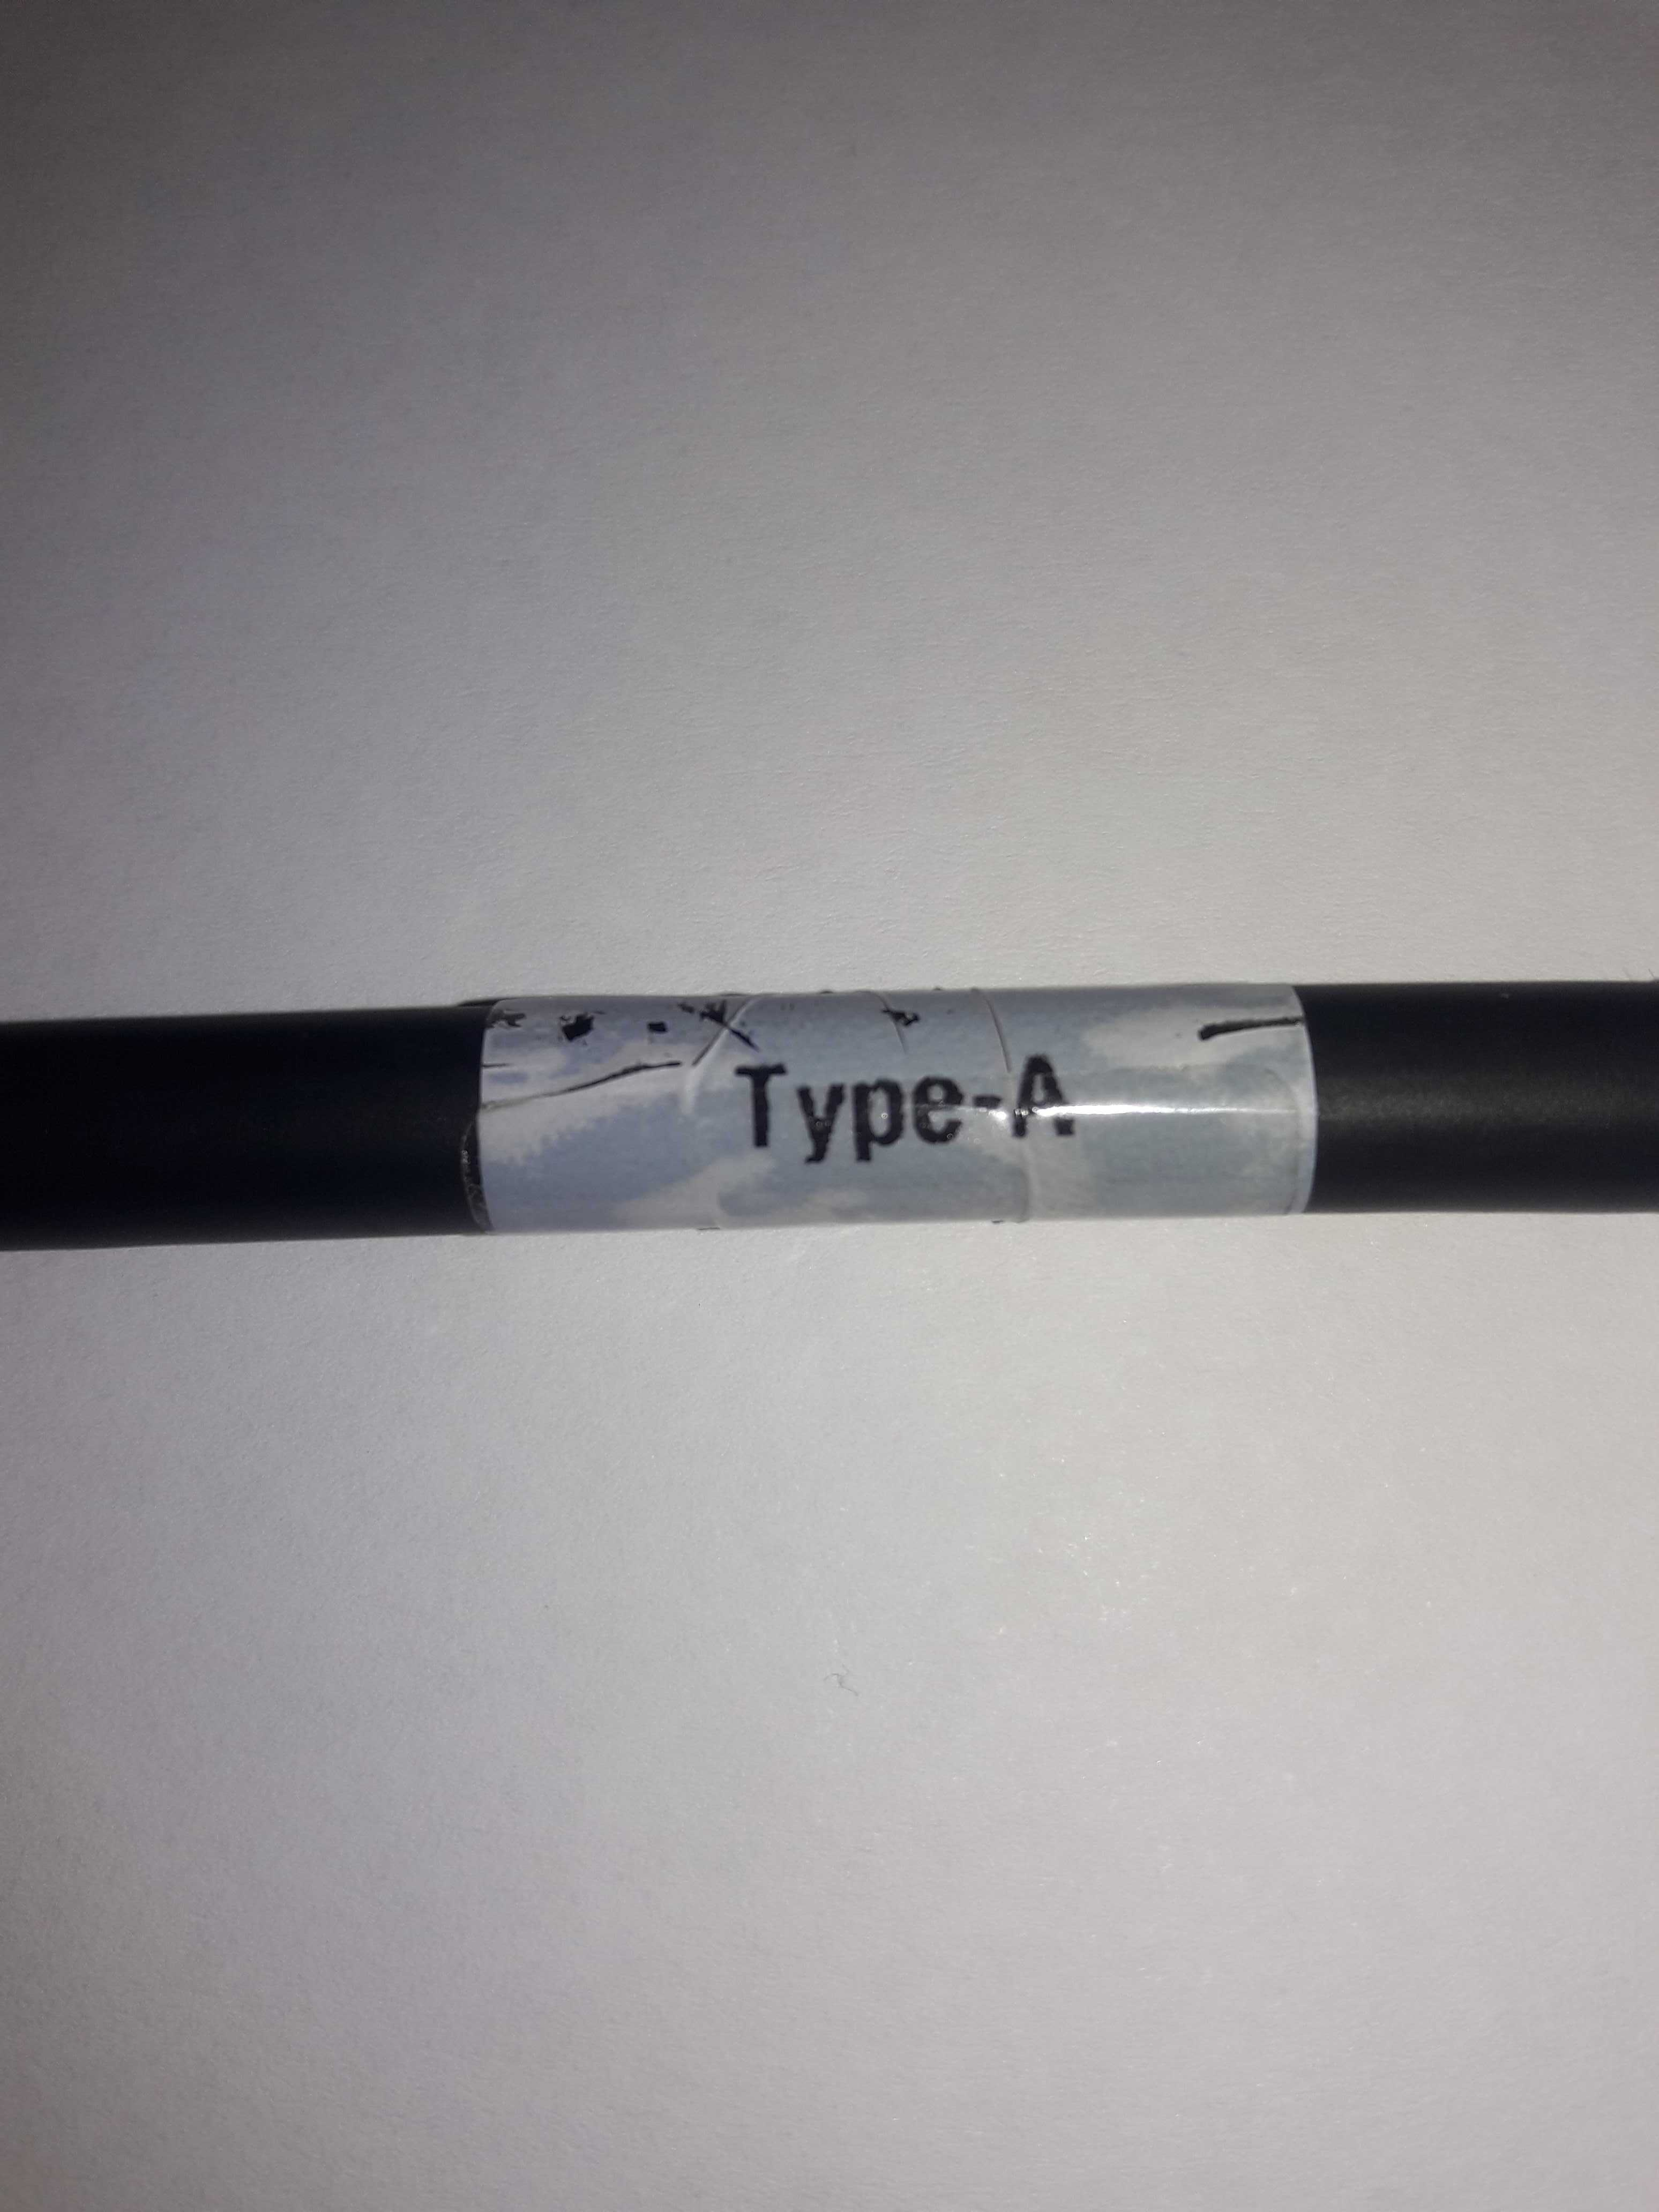
\includegraphics[width=\textwidth]{images/66.jpg}
    \end{subfigure}
    \hfill
    \begin{subfigure}{0.48\textwidth}
      \centering
      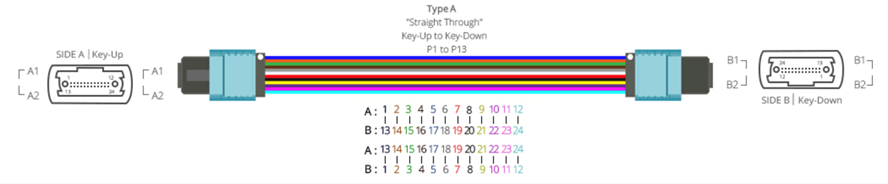
\includegraphics[width=\textwidth]{images/7.png}
    \end{subfigure}
  \end{figure}

\newpage
  %Punto 2.6
  \subsection{Adapter Keys}
  When we refer to the adapter key, it is a notch in the coupler that gives the connection orientation of the connectors. The polarities that are compatible with these adapters are Type A and Type B.
  \begin{itemize}
    \item A Type A adapter or coupler polarity is (Key Up to Key Down)
    \item A Type B adapter or coupler polarity is  (Key Up to Key Up).
  \end{itemize}
  In this report, Type A coupler will be documented.
  \begin{figure}
    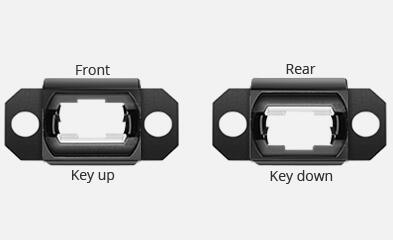
\includegraphics[width=11cm]{images/8.jpg}
    \centering
  \end{figure}

\newpage
  %Punto 2.7
  \subsection{Cable Connection Method}
  To connect these cables we will need to use the corresponding adapter for the polarity of the cable used. The image below illustrates the connection method used for a male-to-female type A cable using a coupler with Flange (Key Up to Down).
  \begin{figure}
    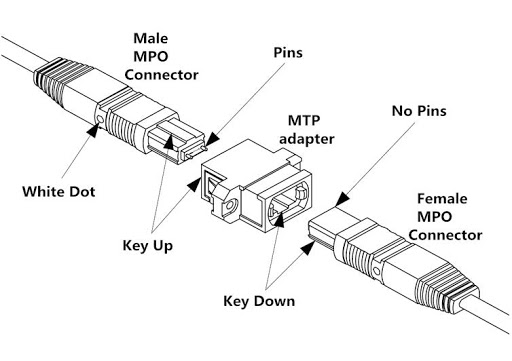
\includegraphics[width=11cm]{images/9.jpg}
    \centering
  \end{figure}

\newpage

  %Punto 2.8
  \subsection{Purchase Method}

  To purchase a specific cable we need to know the type of cable we would like to use, its polarity, and any other feature required. Once all of this information is gathered a company representative is contacted with our requirements and the order is received and processed. The company then proceed to manufacture the cable and Is shipped to Tucson and later to Chile which is received by the IT Team at the AURA Facility all in approximately 2 months.
  We made our first purchase for an MTP / MPO cable with military protection to perform a stress test of the material along with its durability.

\newpage


%Punto 3
\section{Installation and maintenance time of the MTP / MPO cable}

To carry out the installation of the cables, we first need to request authorization within a week in advance to the managers and safety personnel in charge, this whole process is documented on a ticket in Jira. For each day of the work, IT has to fill out a daily activity registration form to document the activities that will be carried out for that particular day of work. This form is then delivered to Rubin Safety personnel who are in charge of authorizing the activity and supervising the work done for any safety hazard.

Each area of work has to be demarcated with cones along with an informative table showing the person's name in charge of the work and the areas that will be closed throughout the work period. IT also has to notify Rubin personnel by radio on channel 3 that work will take place in the area authorized.

The installation of this type of cable can usually take up to 2 days with a workgroup composed of 4 members but maintenance can take up to 3 workdays with the same amount of people, this is because the IT Team has to specifically check and withdraw each cable, taking into account the following considerations.

First, we have to locate the cable we are going to be doing maintenance on or replacing.
Remove the cable from where it's currently installed and located.
Prepare and install the new cable in replacement for the one that was removed.


Note: The times provided above are all estimates and takes into account that the cables are installed in the computer room in rack B6 and extend to the sixth floor of the pier where the disconnection point is located at "ACXa". From here the cable is then routed along with the azimuth drape to the 7th floor and ends up at the disconnect location named "AC4" where is then later routed to the top of the telescope.

\newpage
  
  \subsection{IT Camera Fiber Requirements}

  \begin{itemize}
    \item Install the 13 cables from the computer room to the top of the telescope where the TMA structure is located. 
    \item Install 3 additional spare cables for scalability from the computer room to the panel named ACXa located in the 6th floor of the Observatory.
    \item One of these cables will be set apart for the CCS connection. 
  \end{itemize}

  \subsection{MTP cable routing analysis}
  \begin{figure}
    \centering
    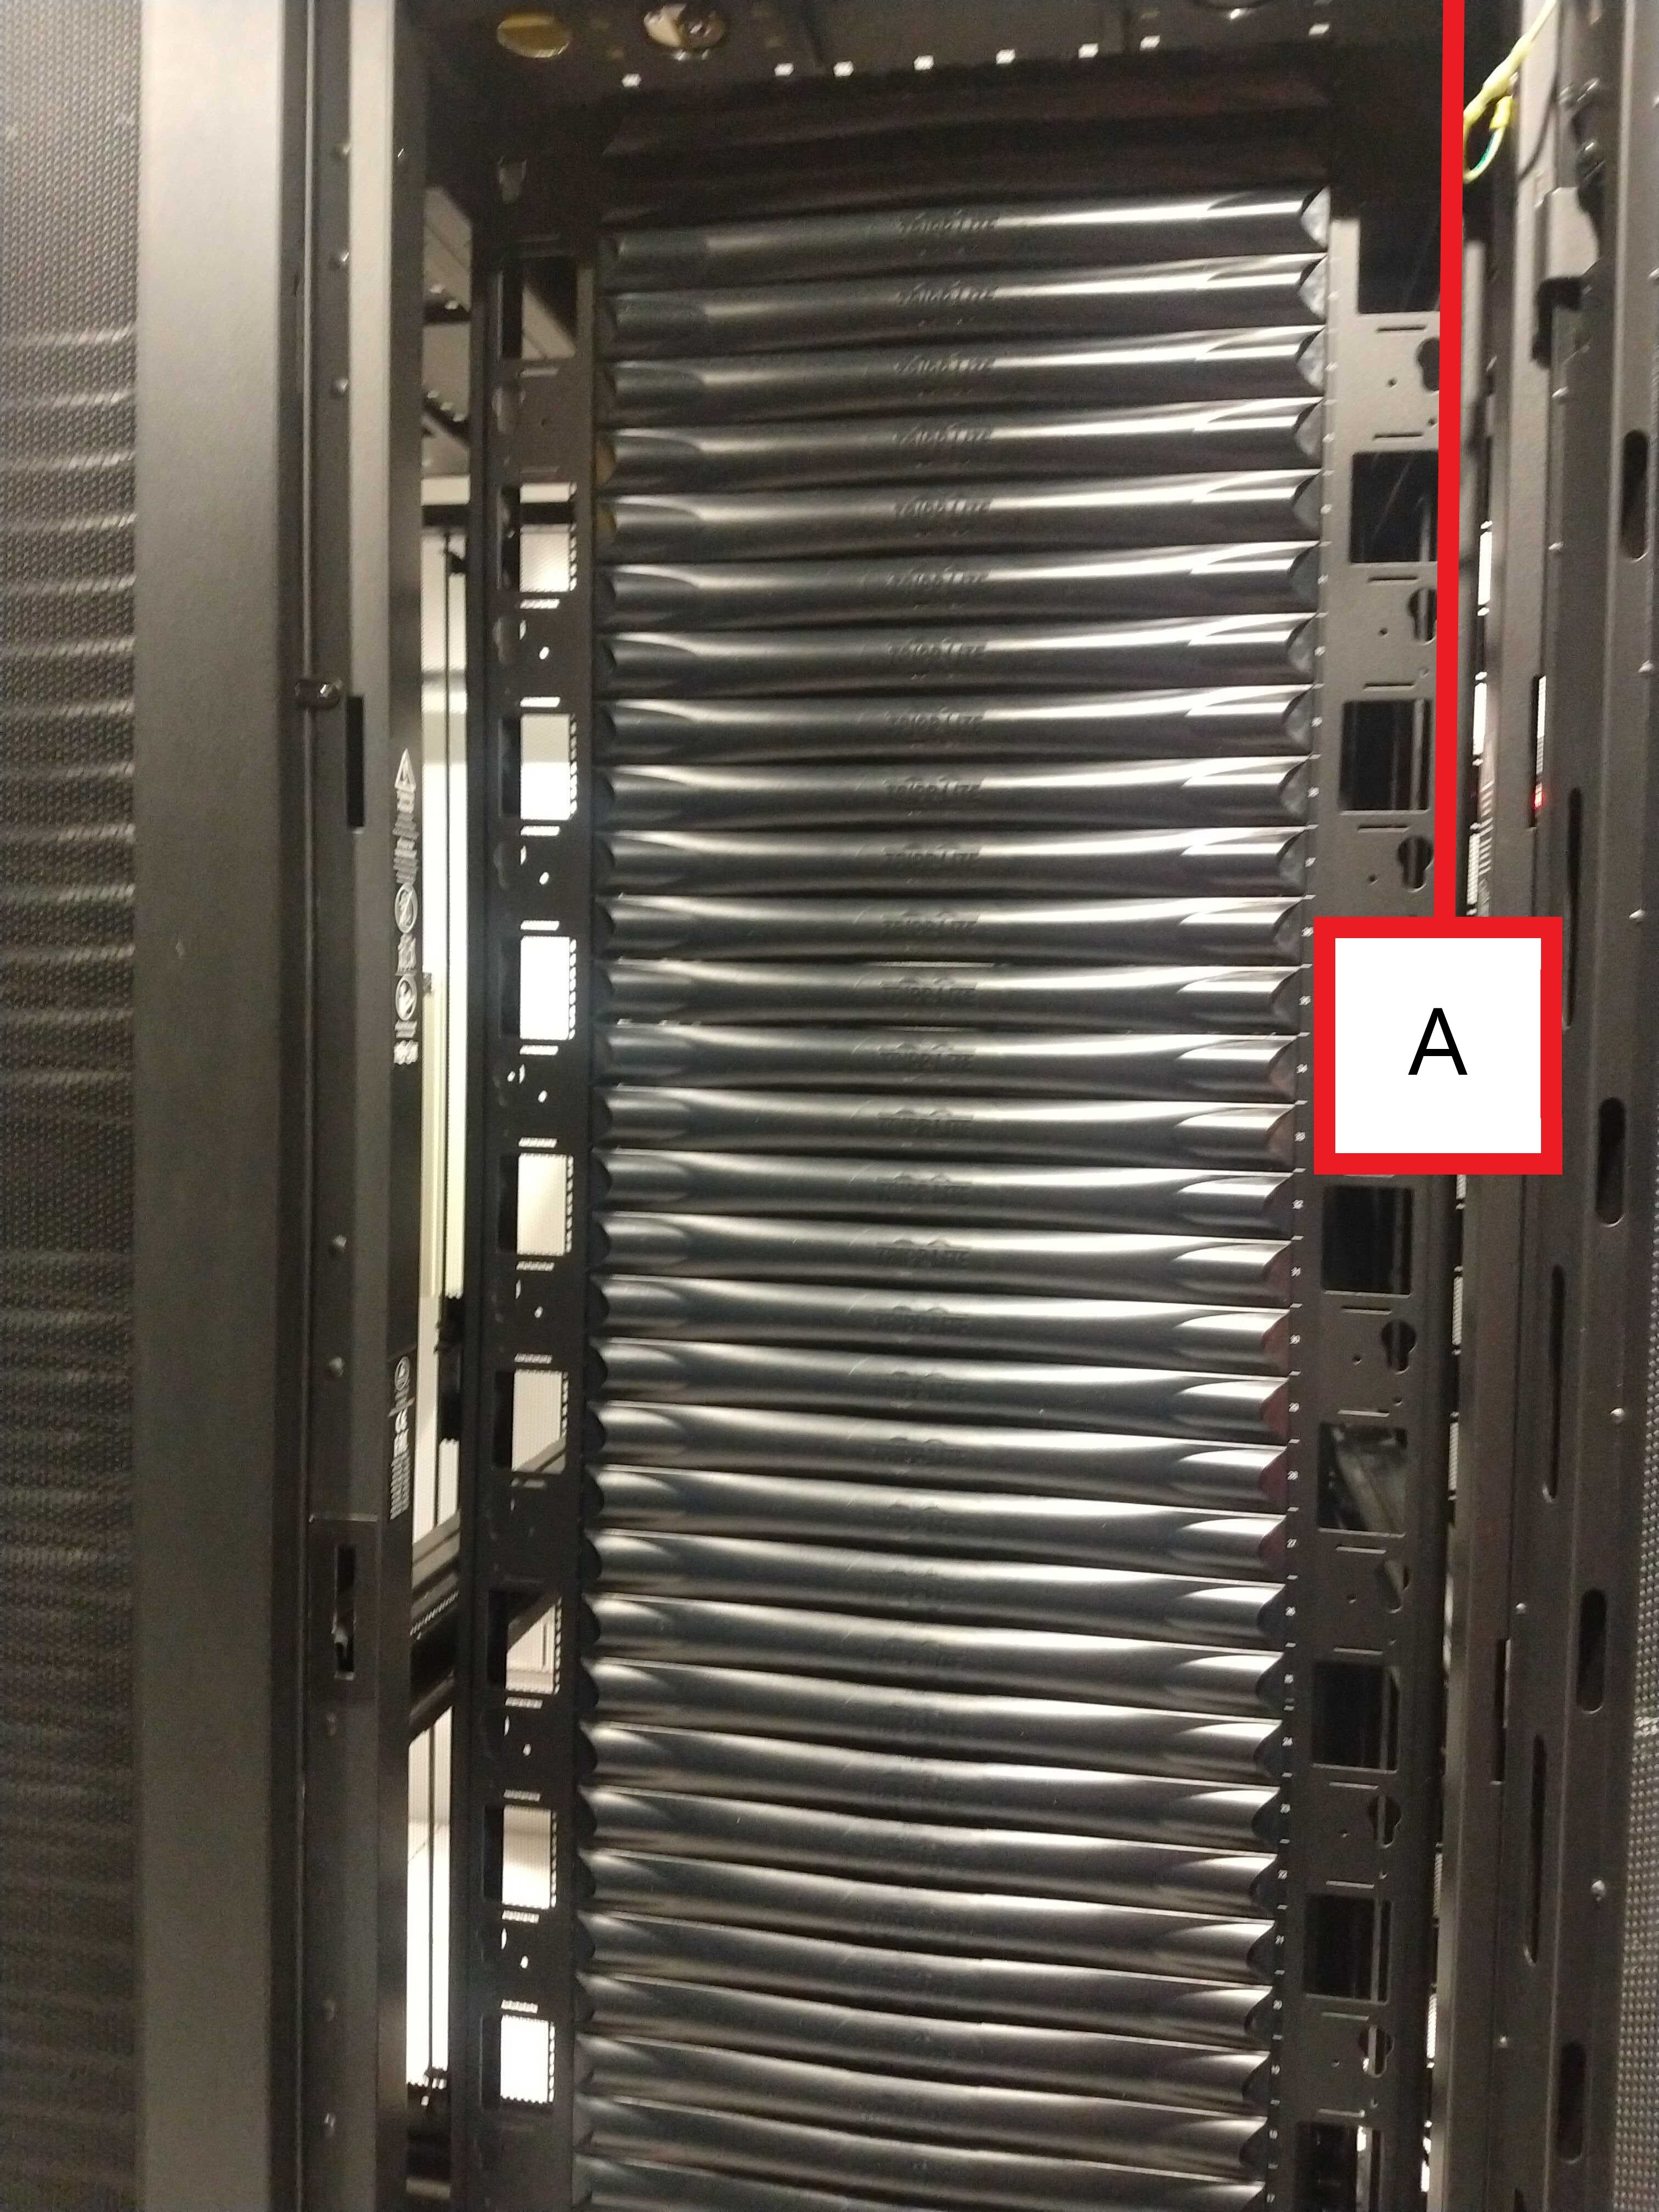
\includegraphics[width=9cm]{images/111.jpg}
    \caption*{The DAQ rack will be located in the data center at Pachon.} 
  \end{figure}

\newpage

  \begin{figure}
    \centering
    \begin{subfigure}{0.40\textwidth}
      \centering
      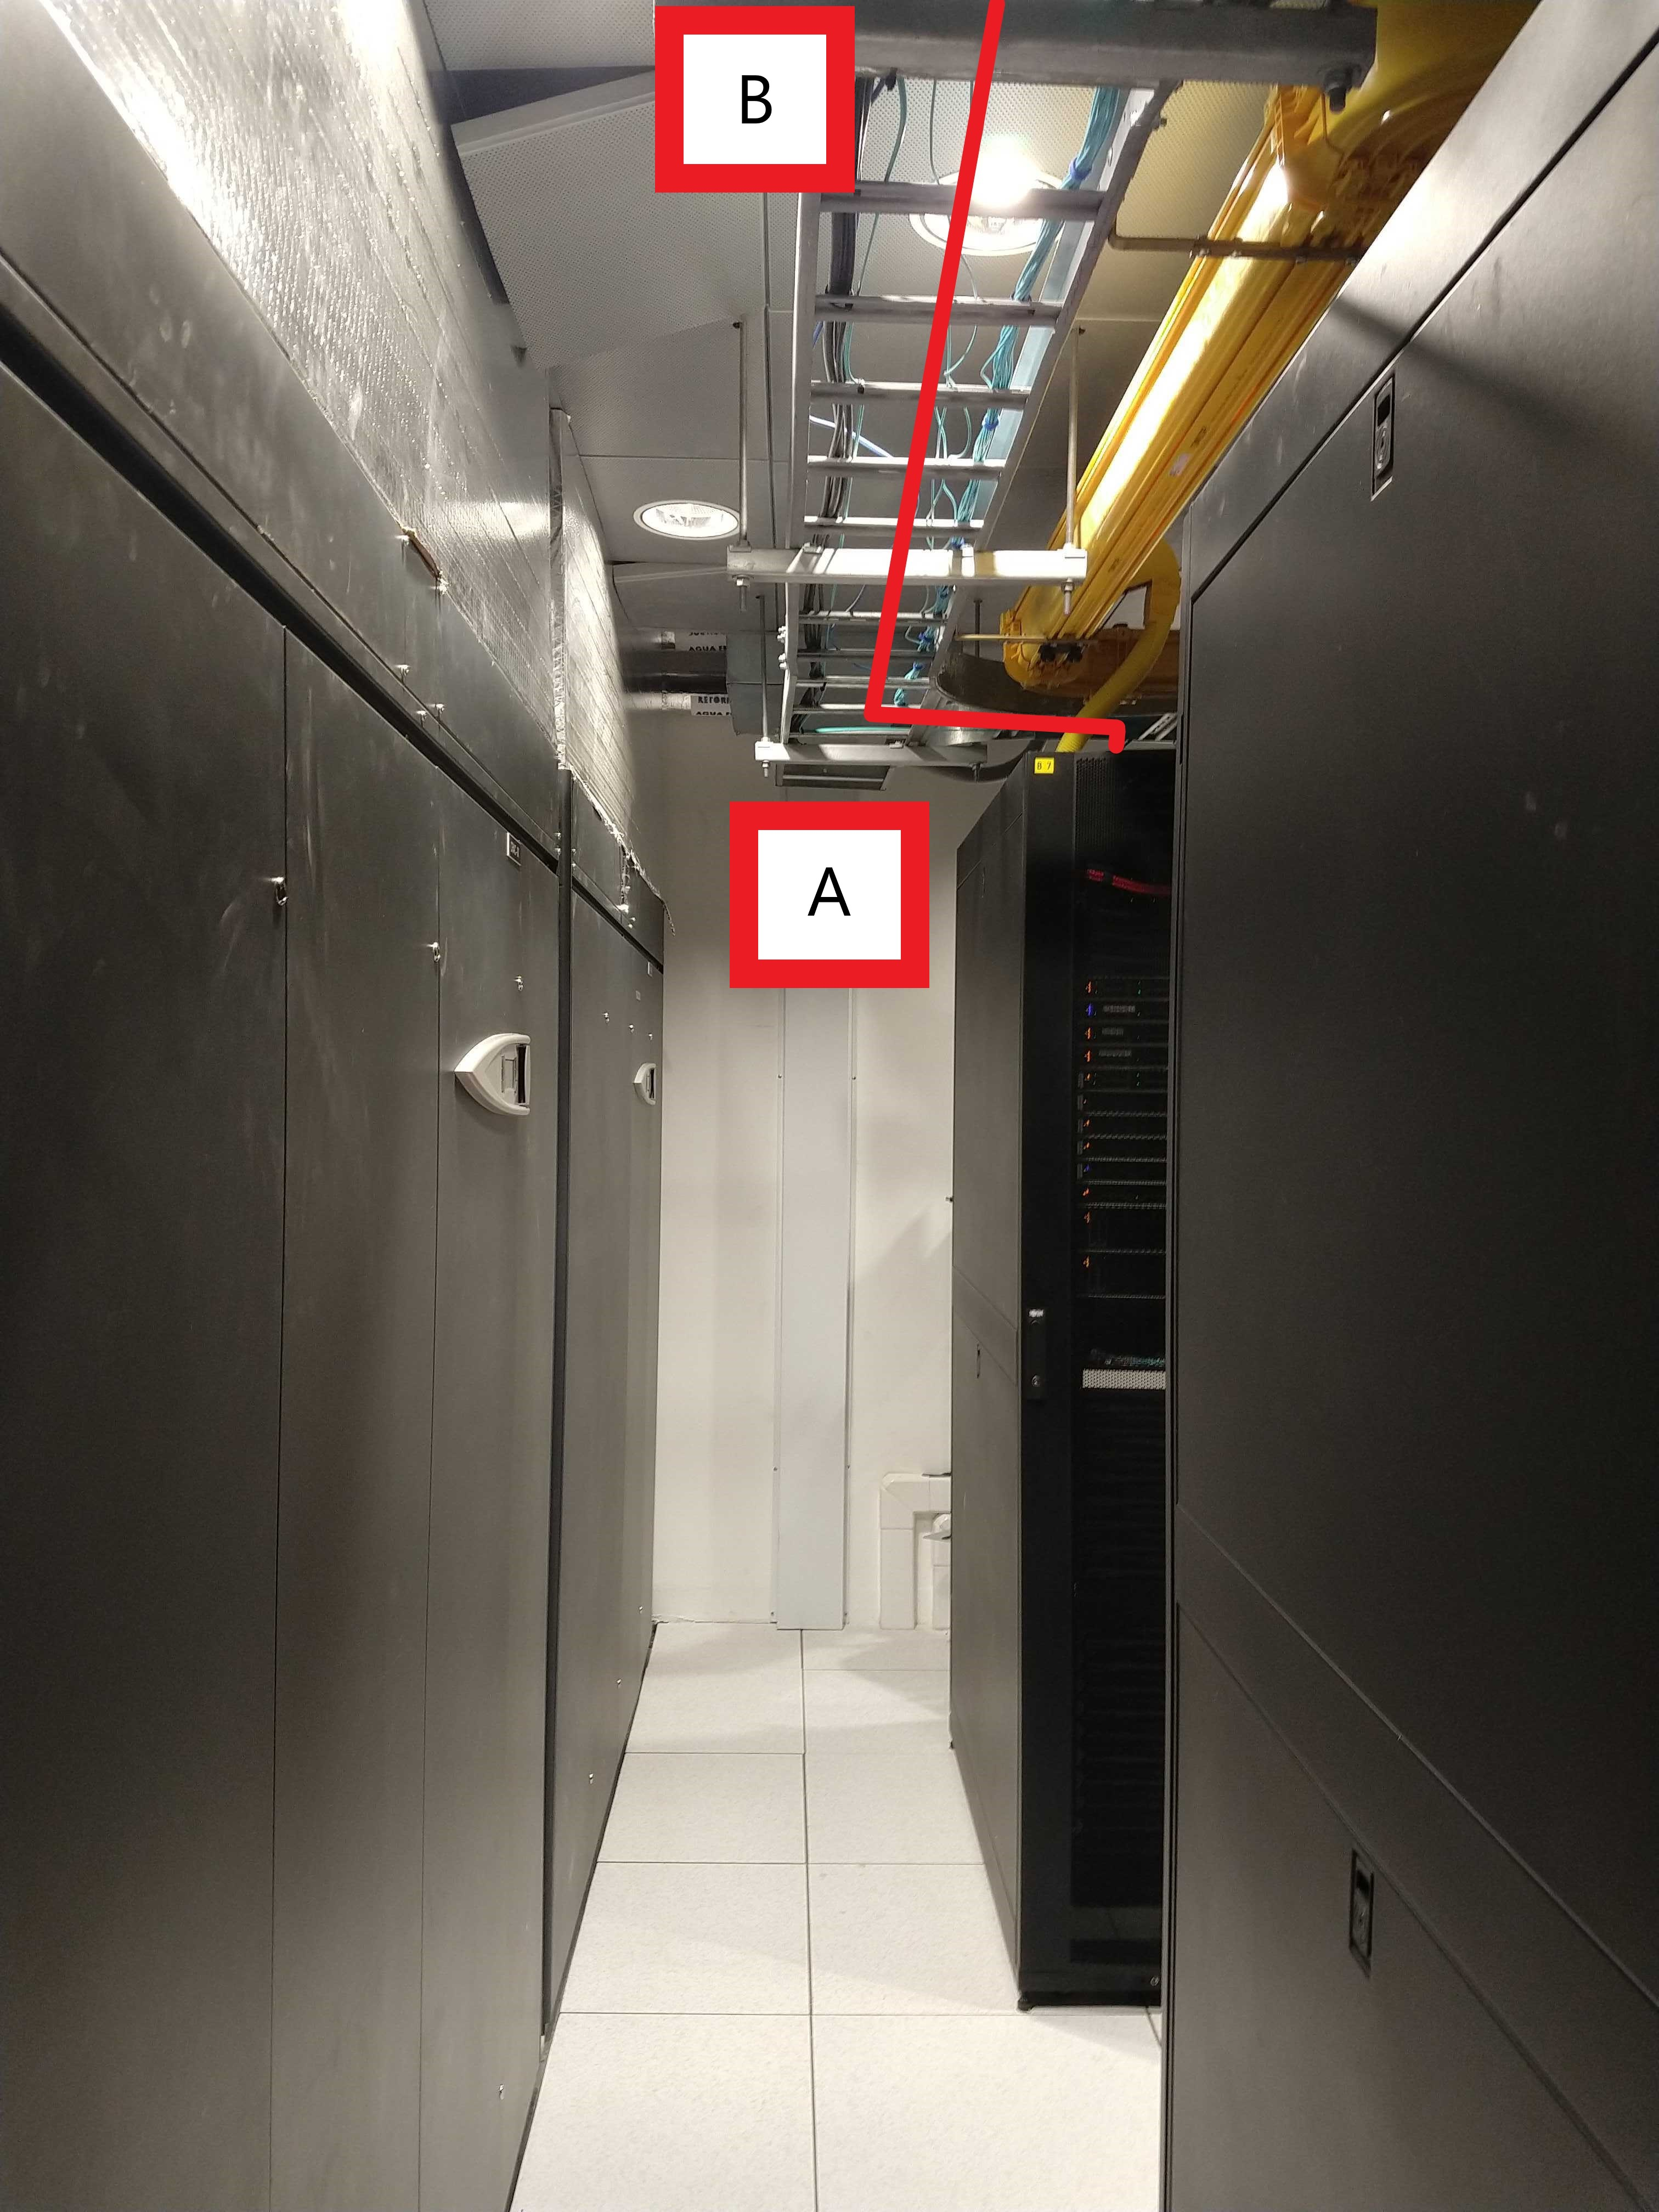
\includegraphics[width=\textwidth]{images/11.jpg}
    \end{subfigure}
      \hfill
    \begin{subfigure}{0.40\textwidth}
      \centering
      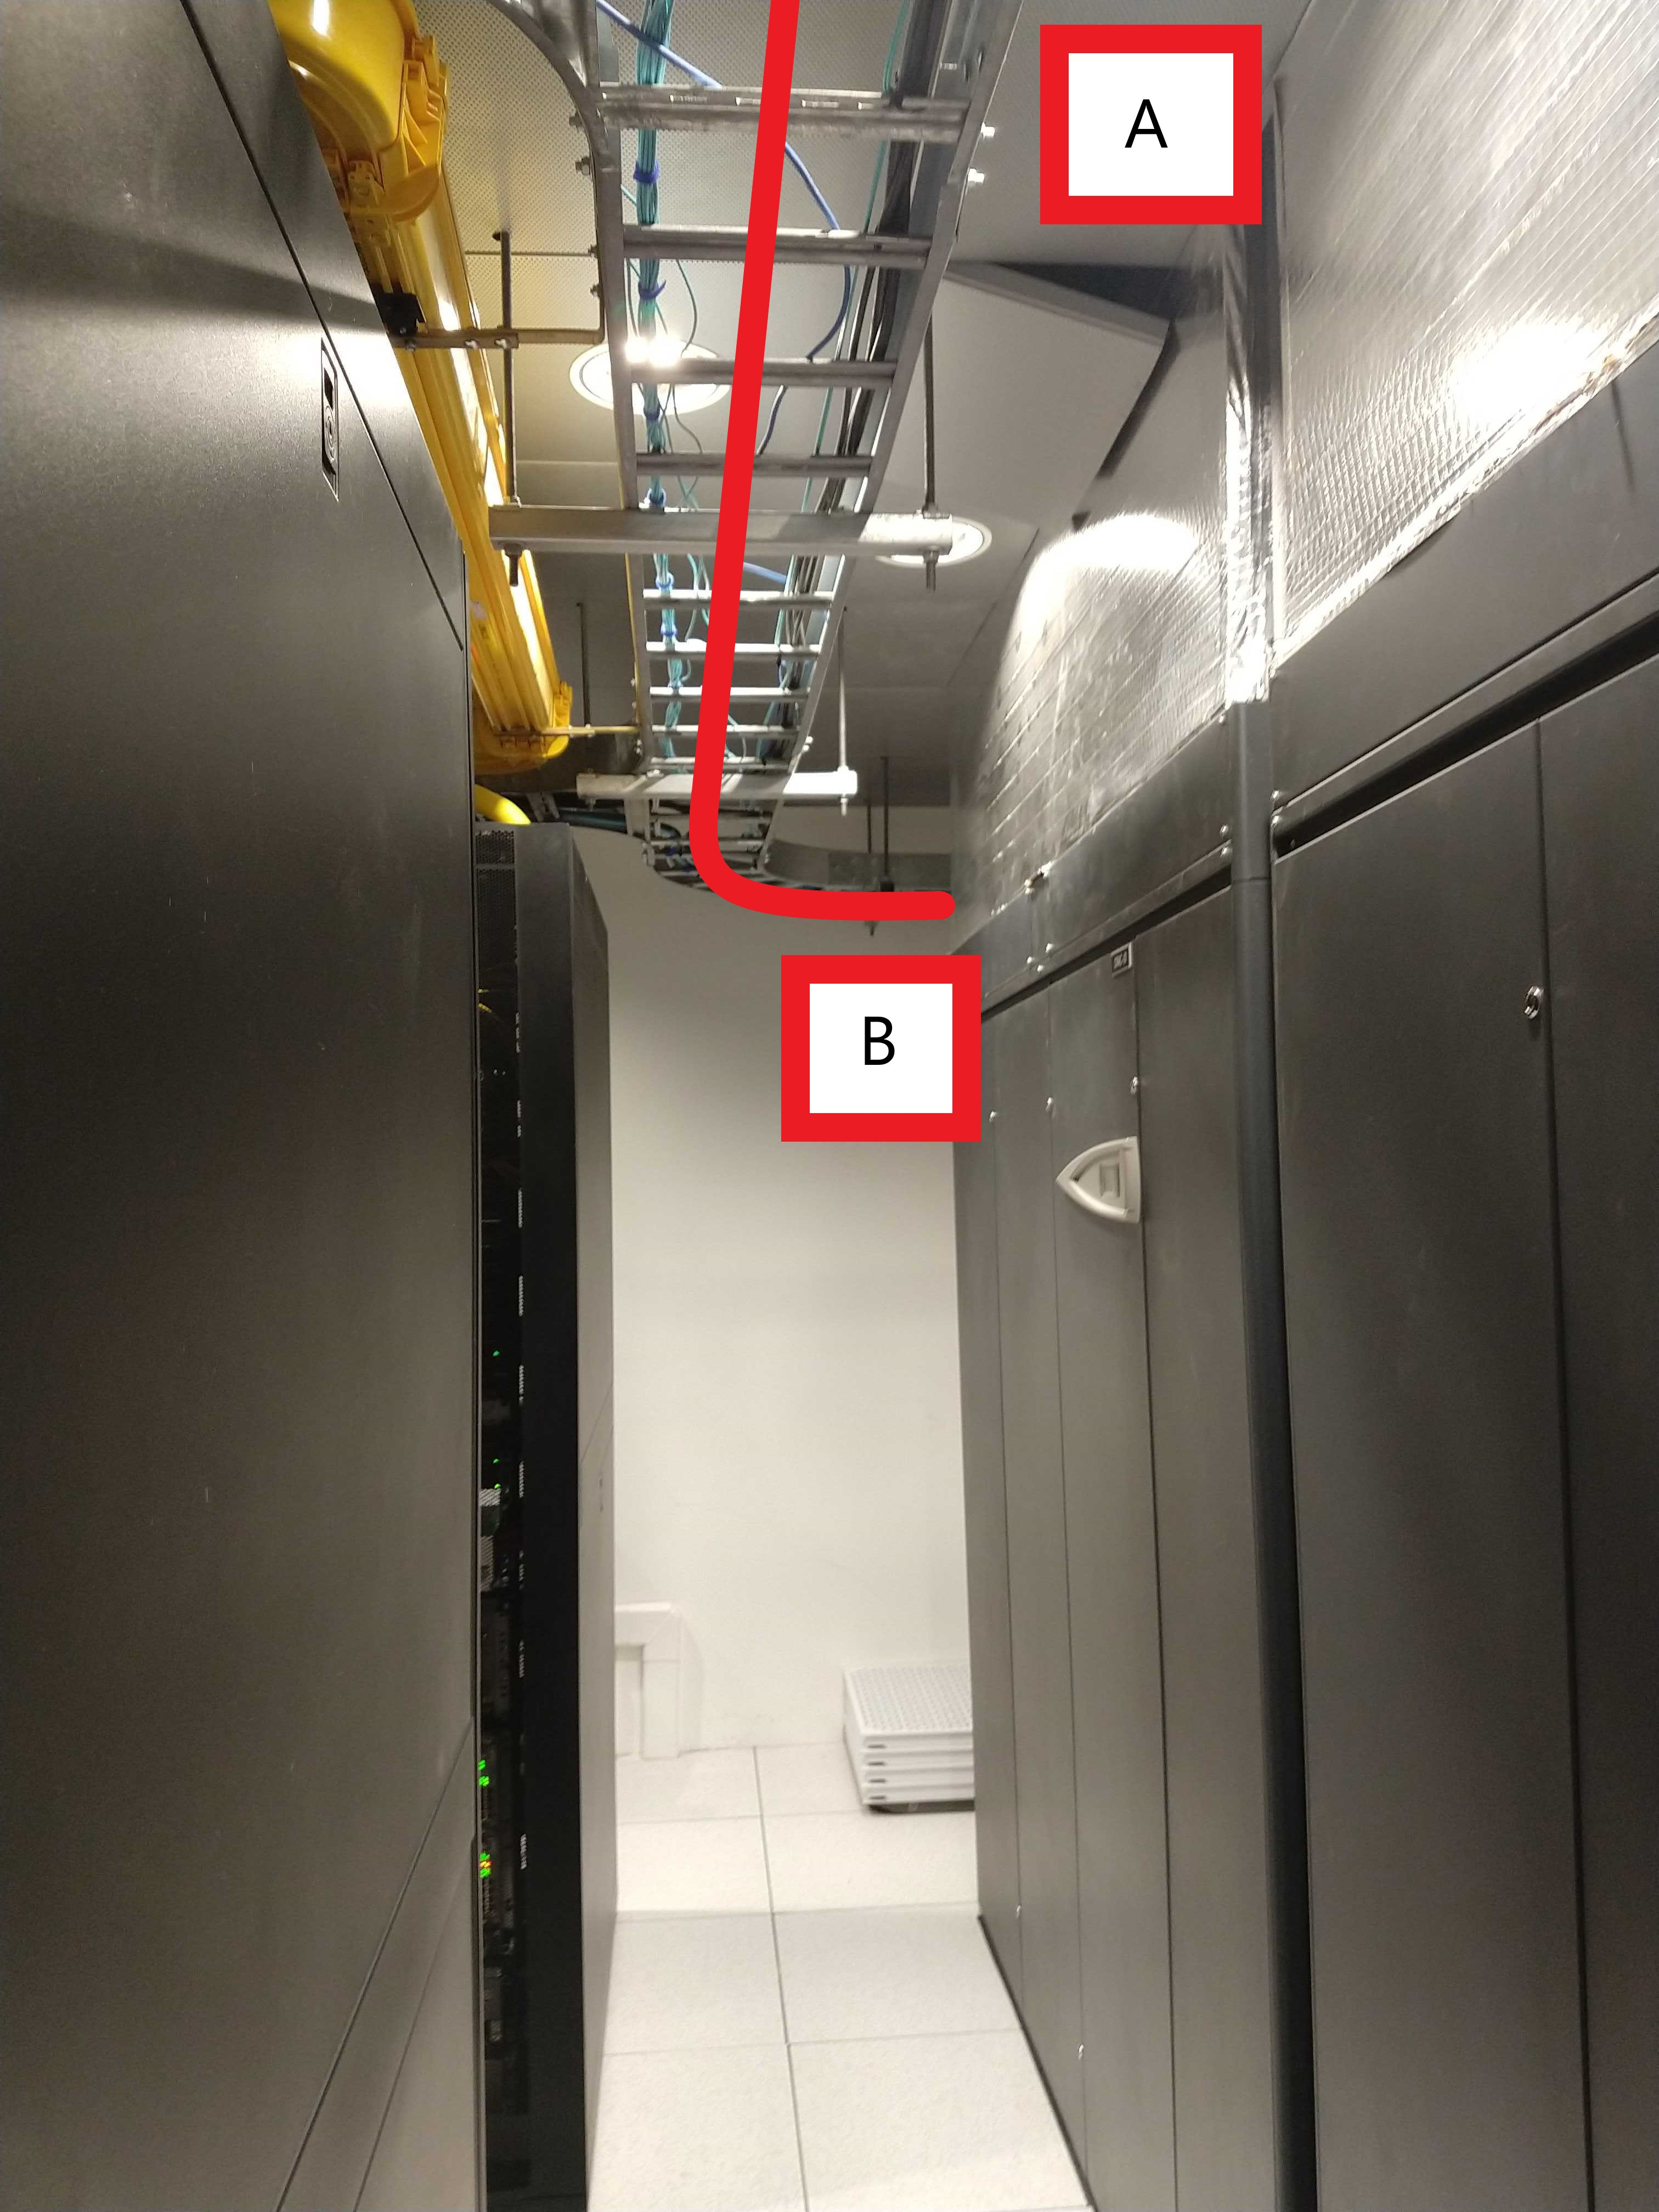
\includegraphics[width=\textwidth]{images/12.jpg}
    \end{subfigure}
  \end{figure}
  The cable originates and exists out of the top of rack B6 at position A of the computer room. The cable then runs through the cable tray in the same room to position B of the computer room exiting at the end of the room.
  
\newpage

  \begin{figure}
    \centering
    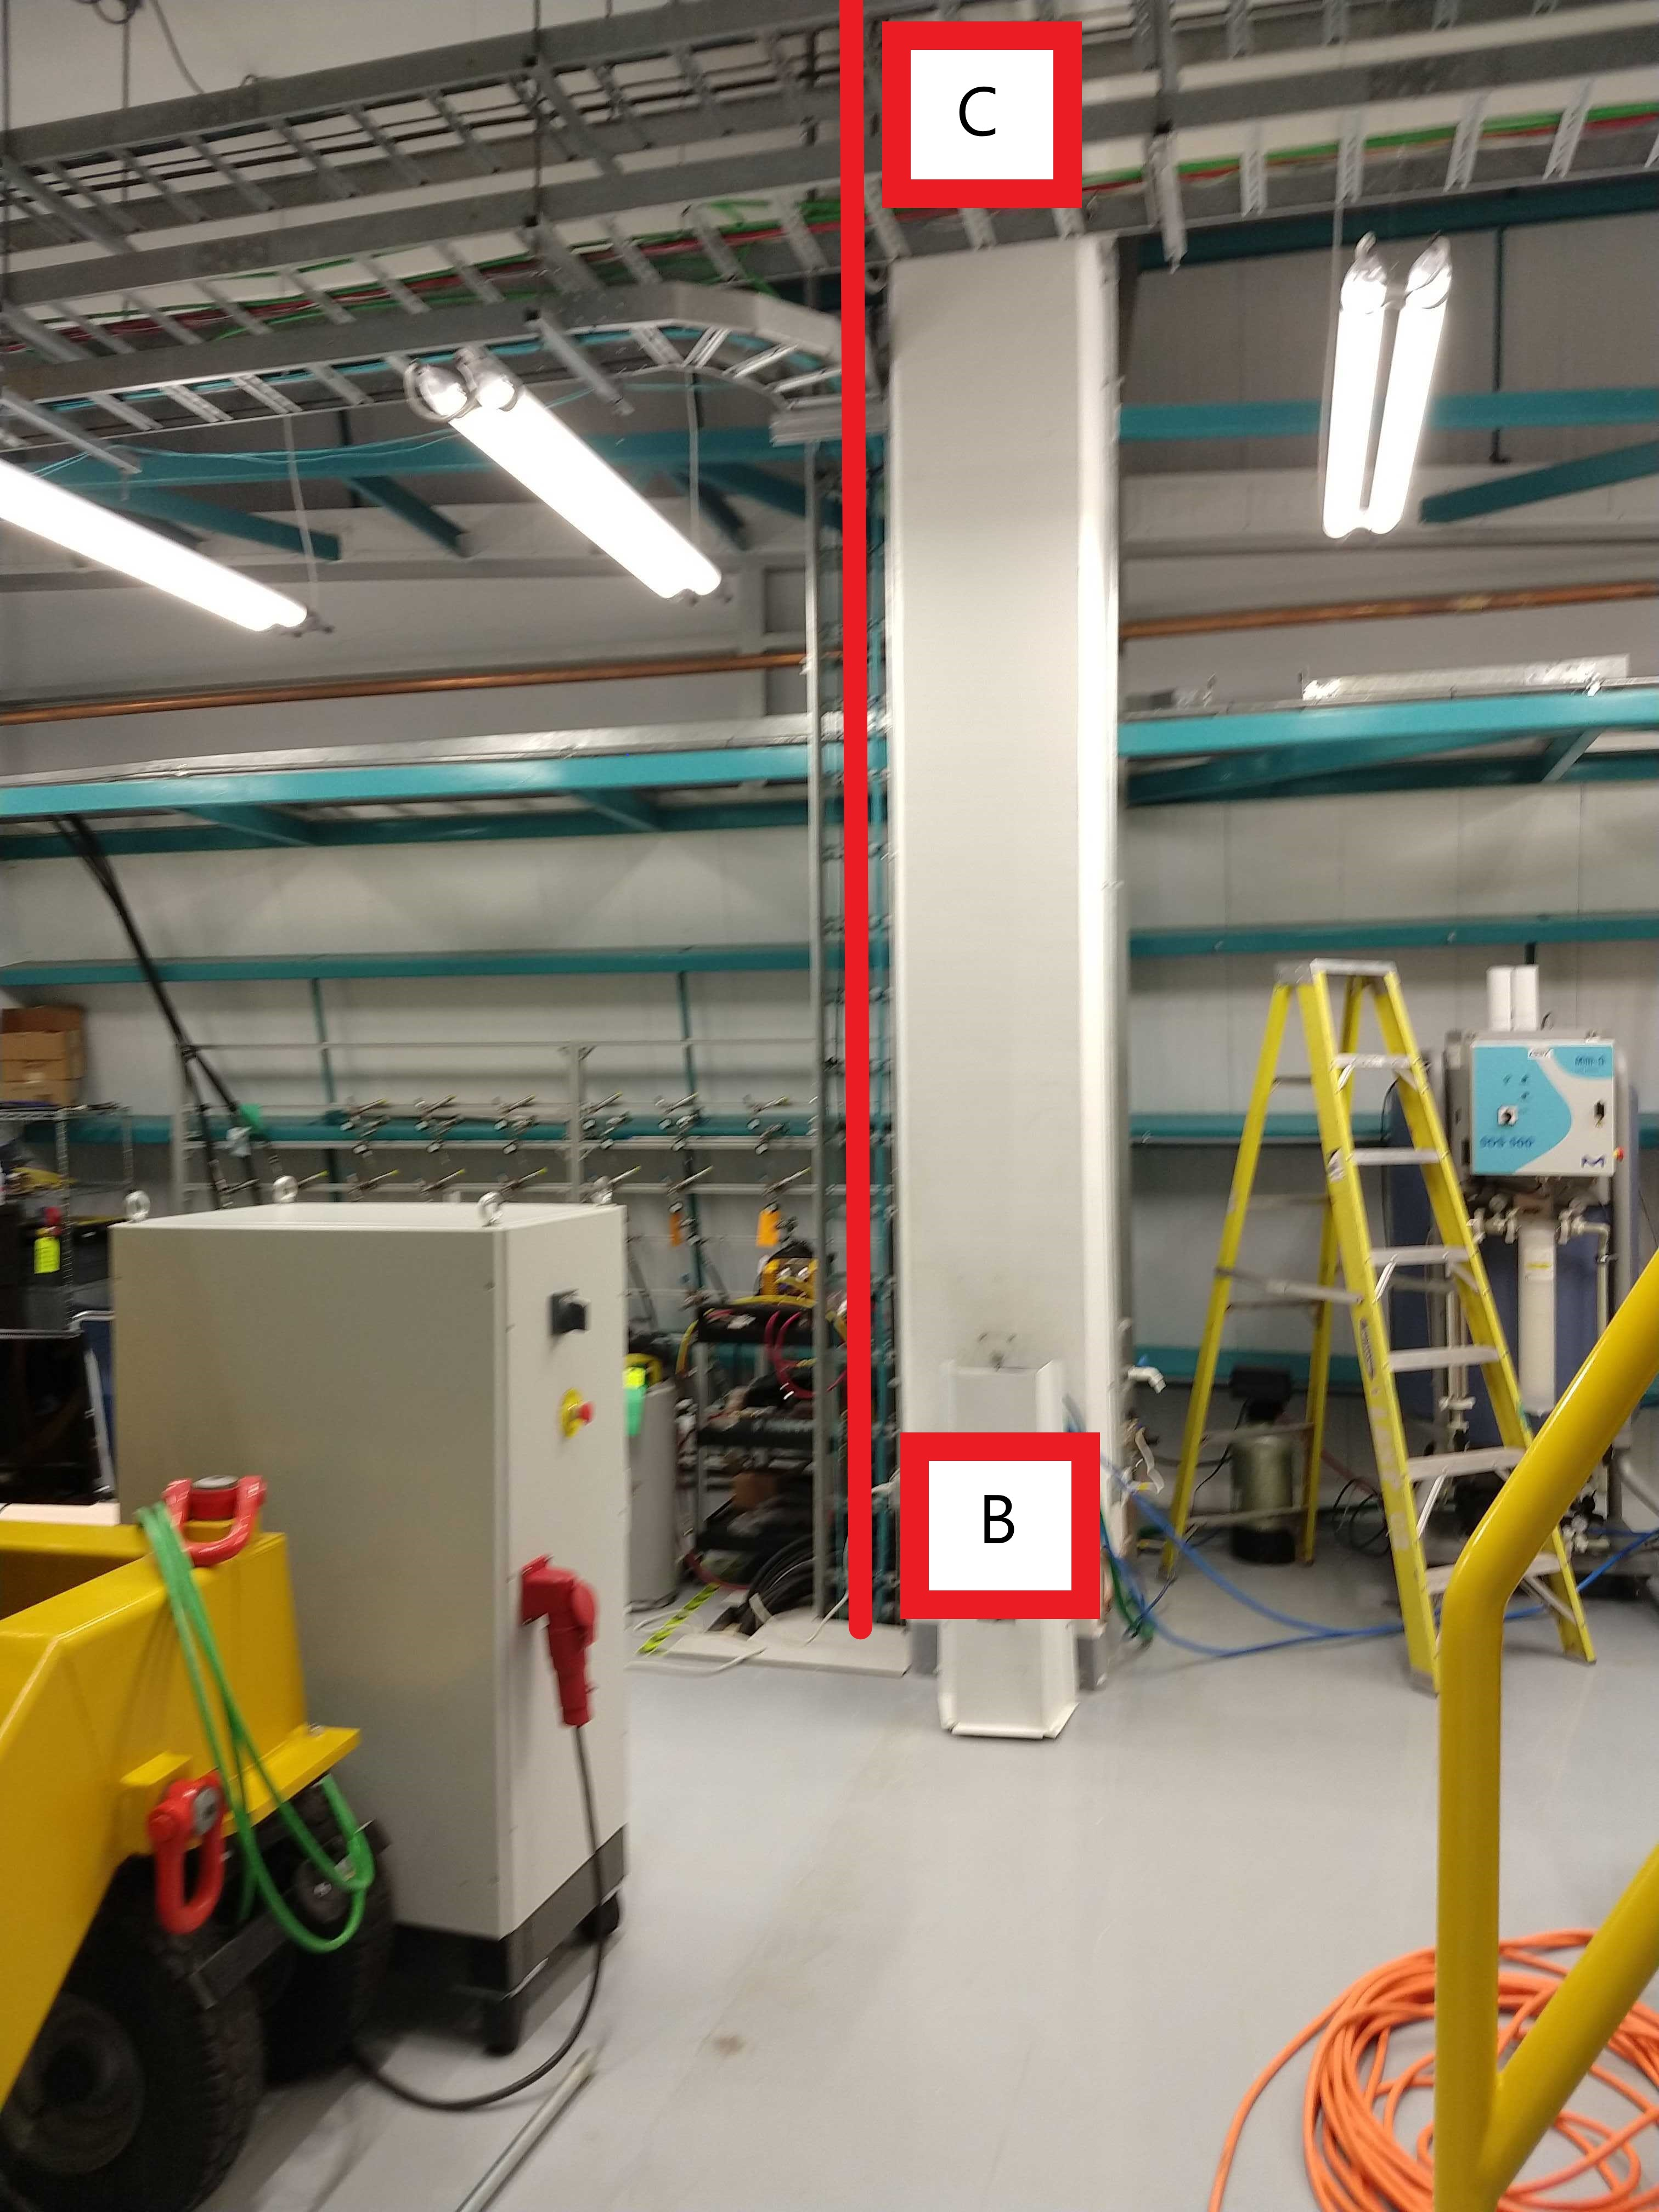
\includegraphics[width=10cm]{images/13.jpg}
  \end{figure}
  The cable then appears on the cable tray of the third floor and runs along the pillar to point C extending to the floor above.

\newpage

  \begin{figure}
    \centering
    \begin{subfigure}{0.45\textwidth}
      \centering
      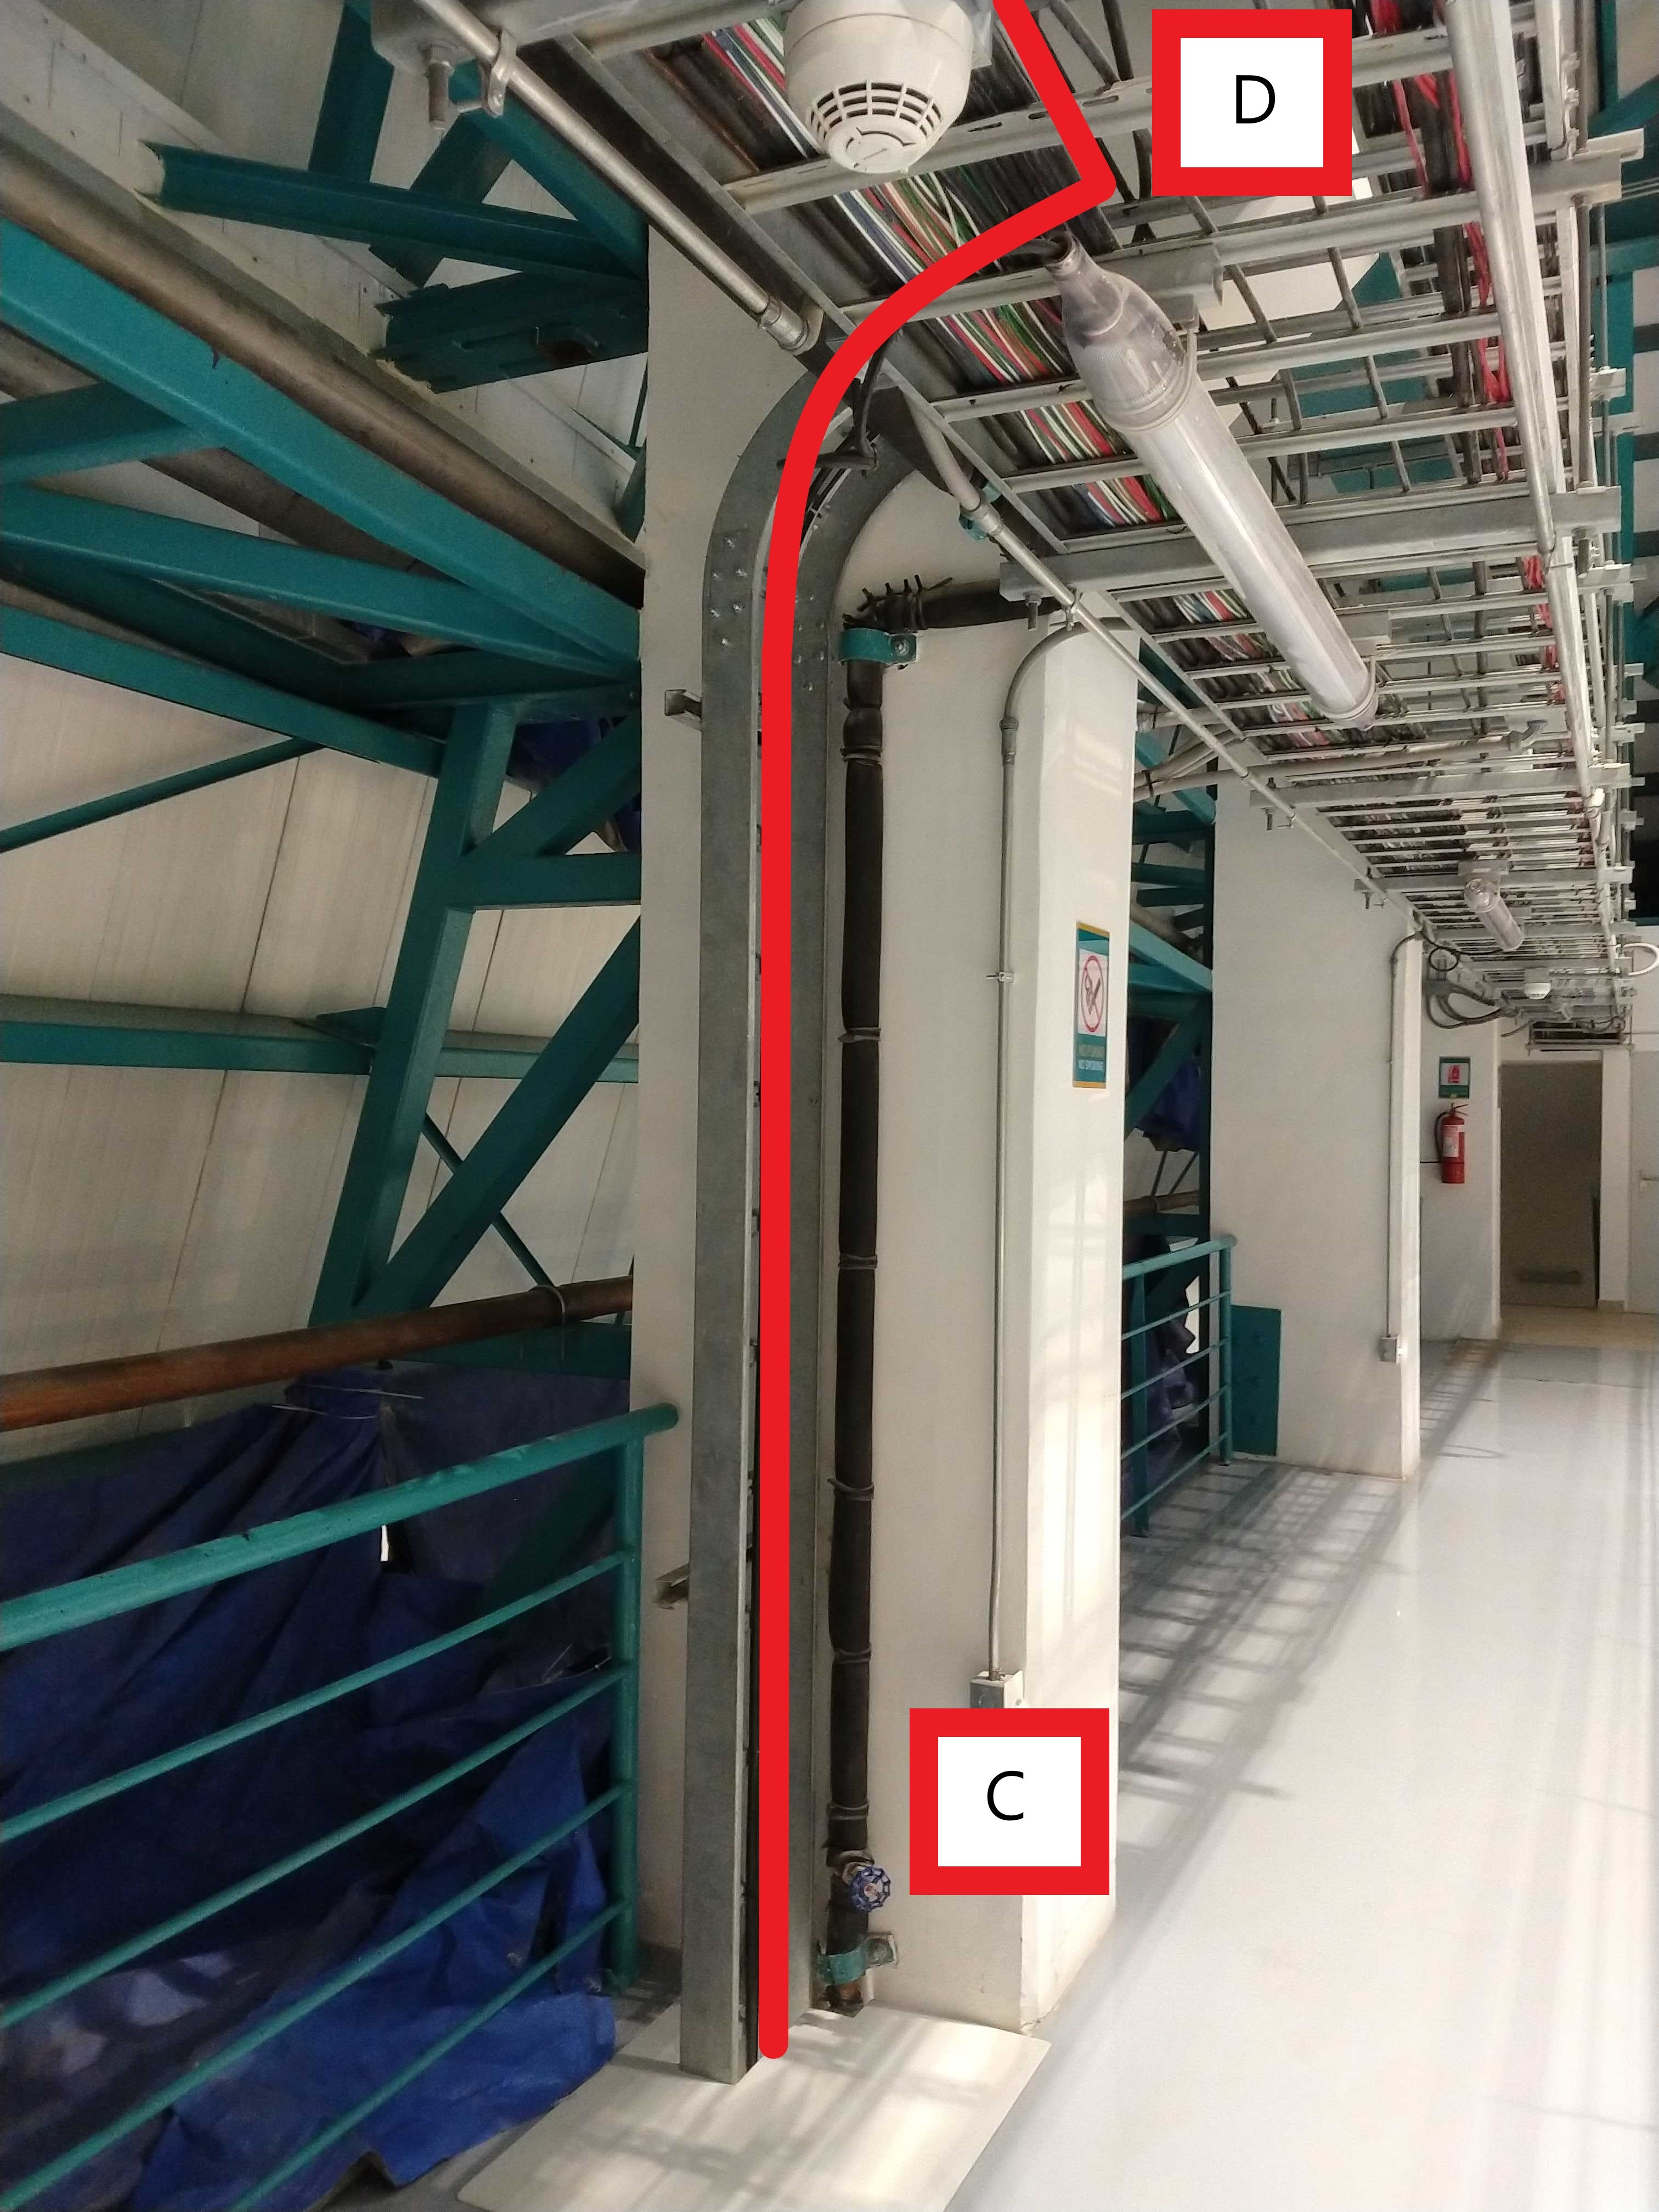
\includegraphics[width=\textwidth]{images/14.jpg}
    \end{subfigure}
    \hfill
    \begin{subfigure}{0.45\textwidth}
      \centering
      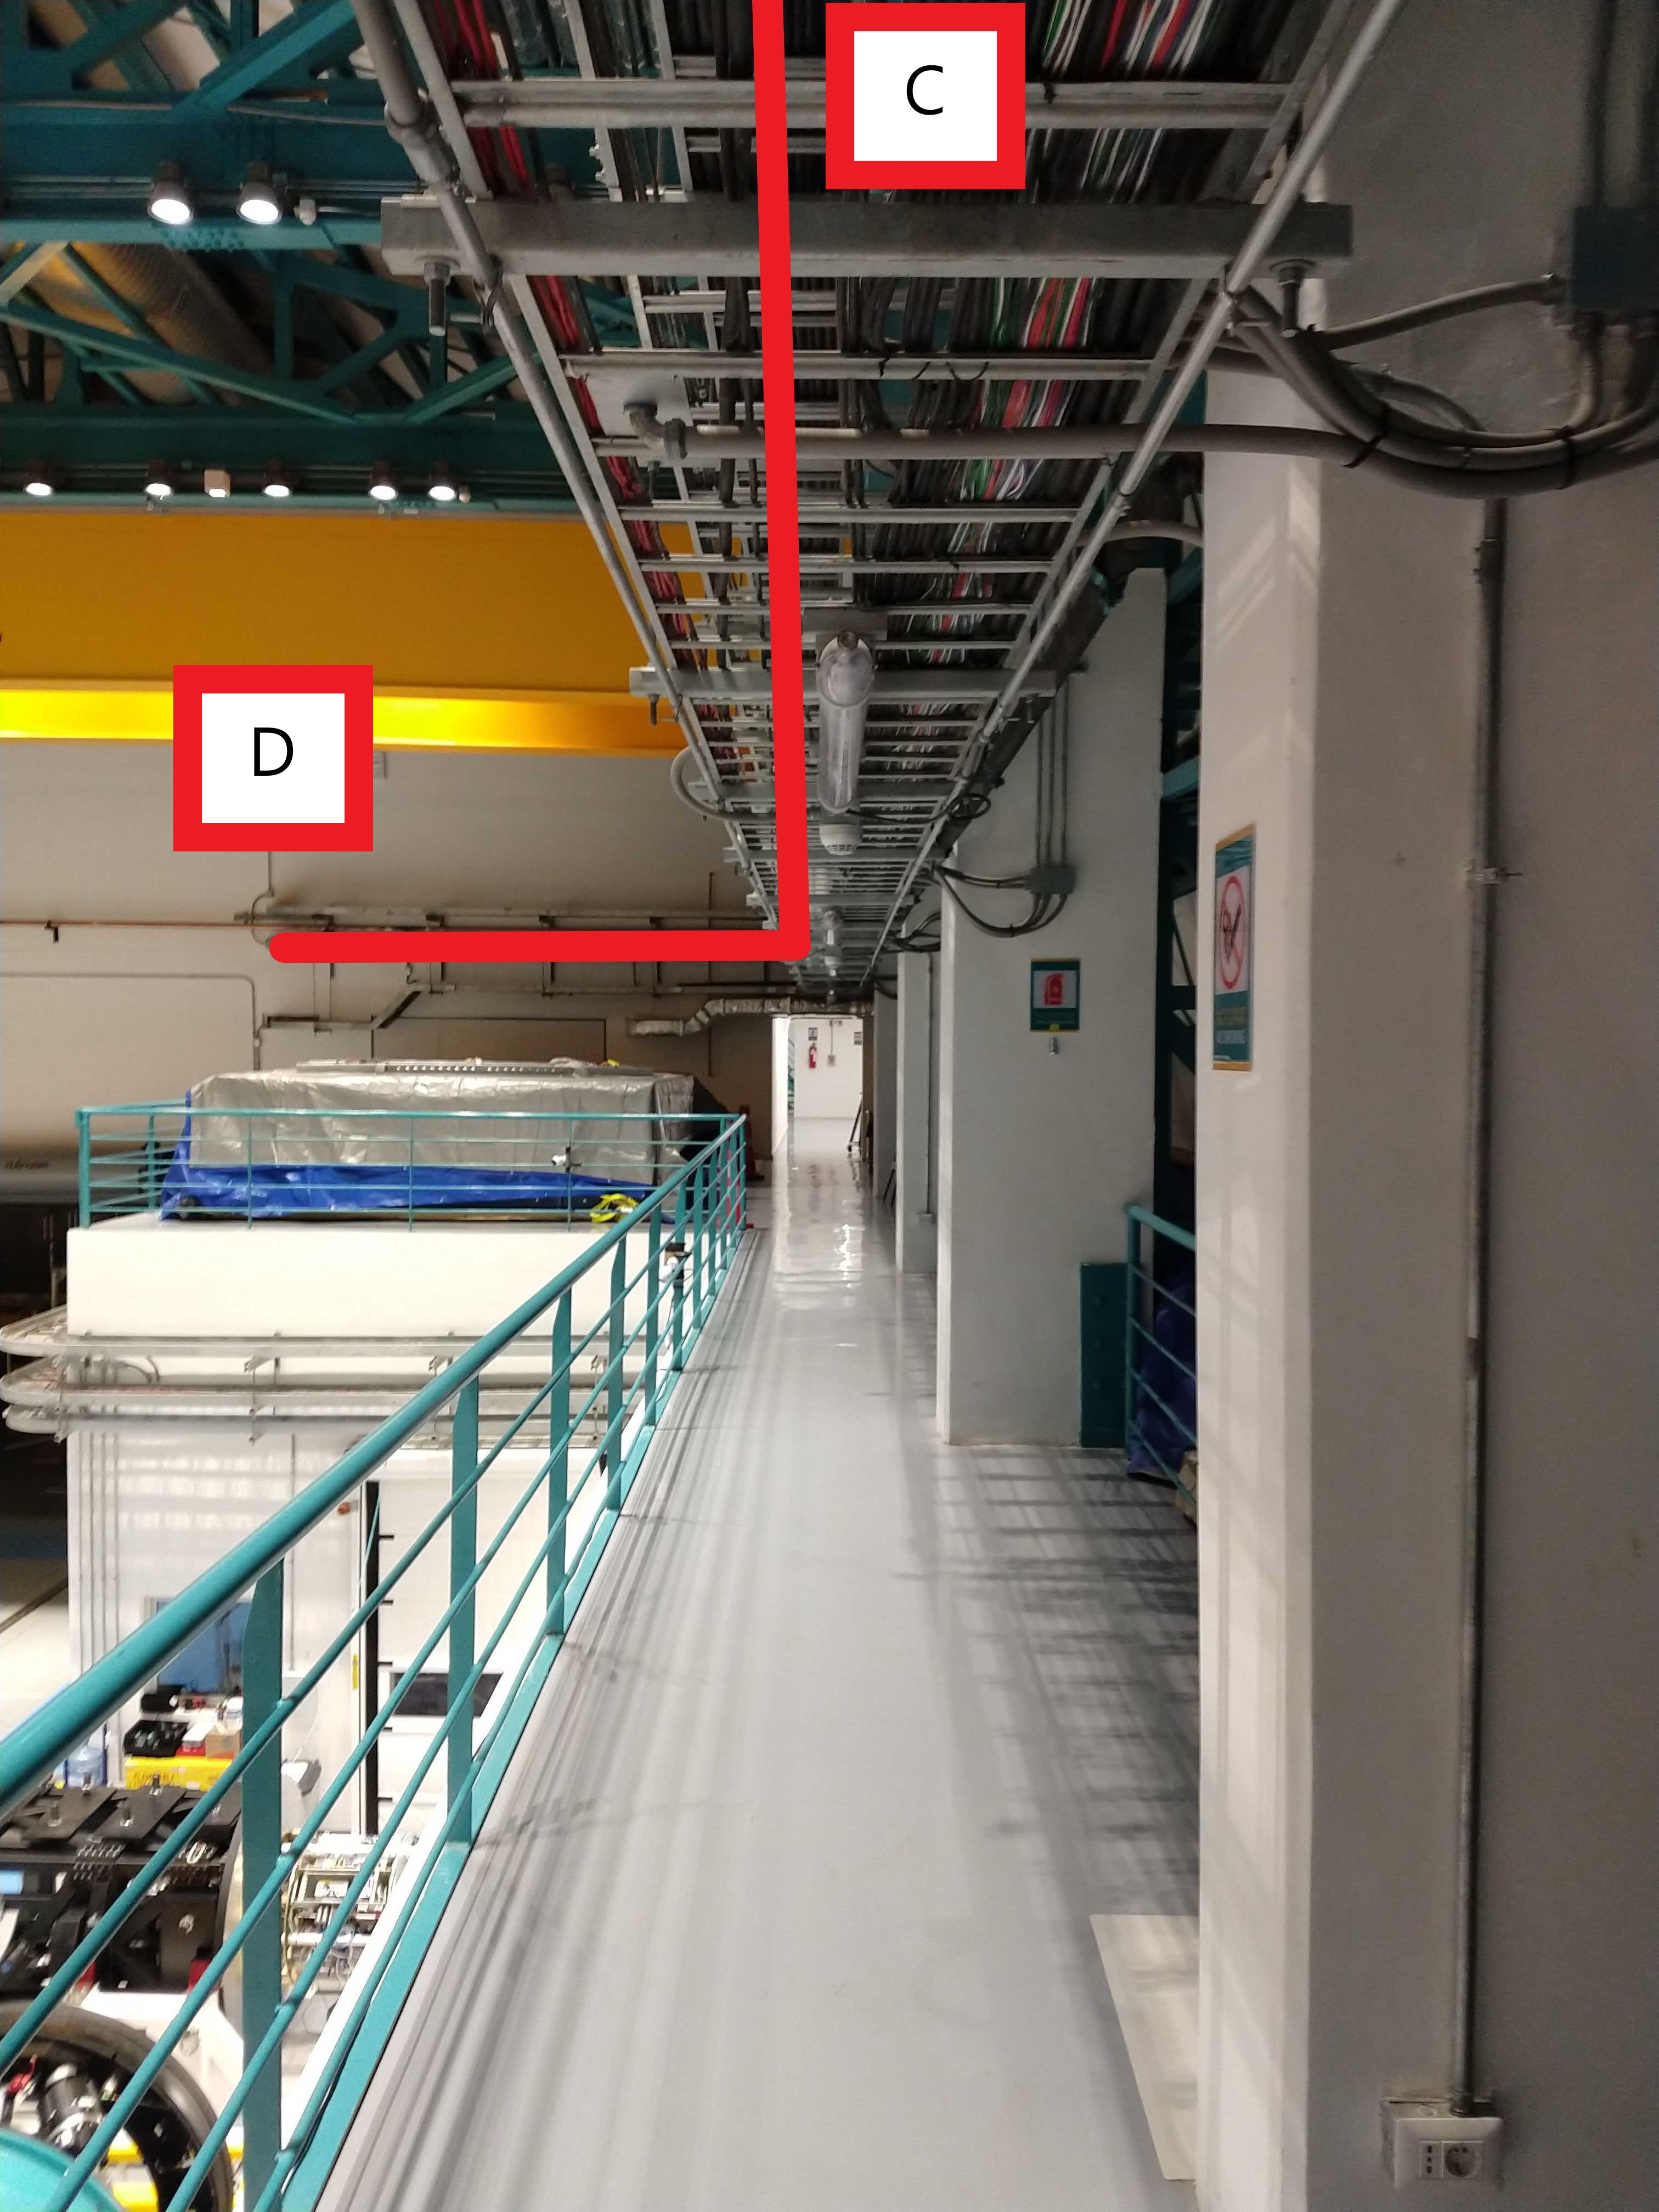
\includegraphics[width=\textwidth]{images/15.jpg}
    \end{subfigure}
  \end{figure}
  \begin{figure}
    \centering
    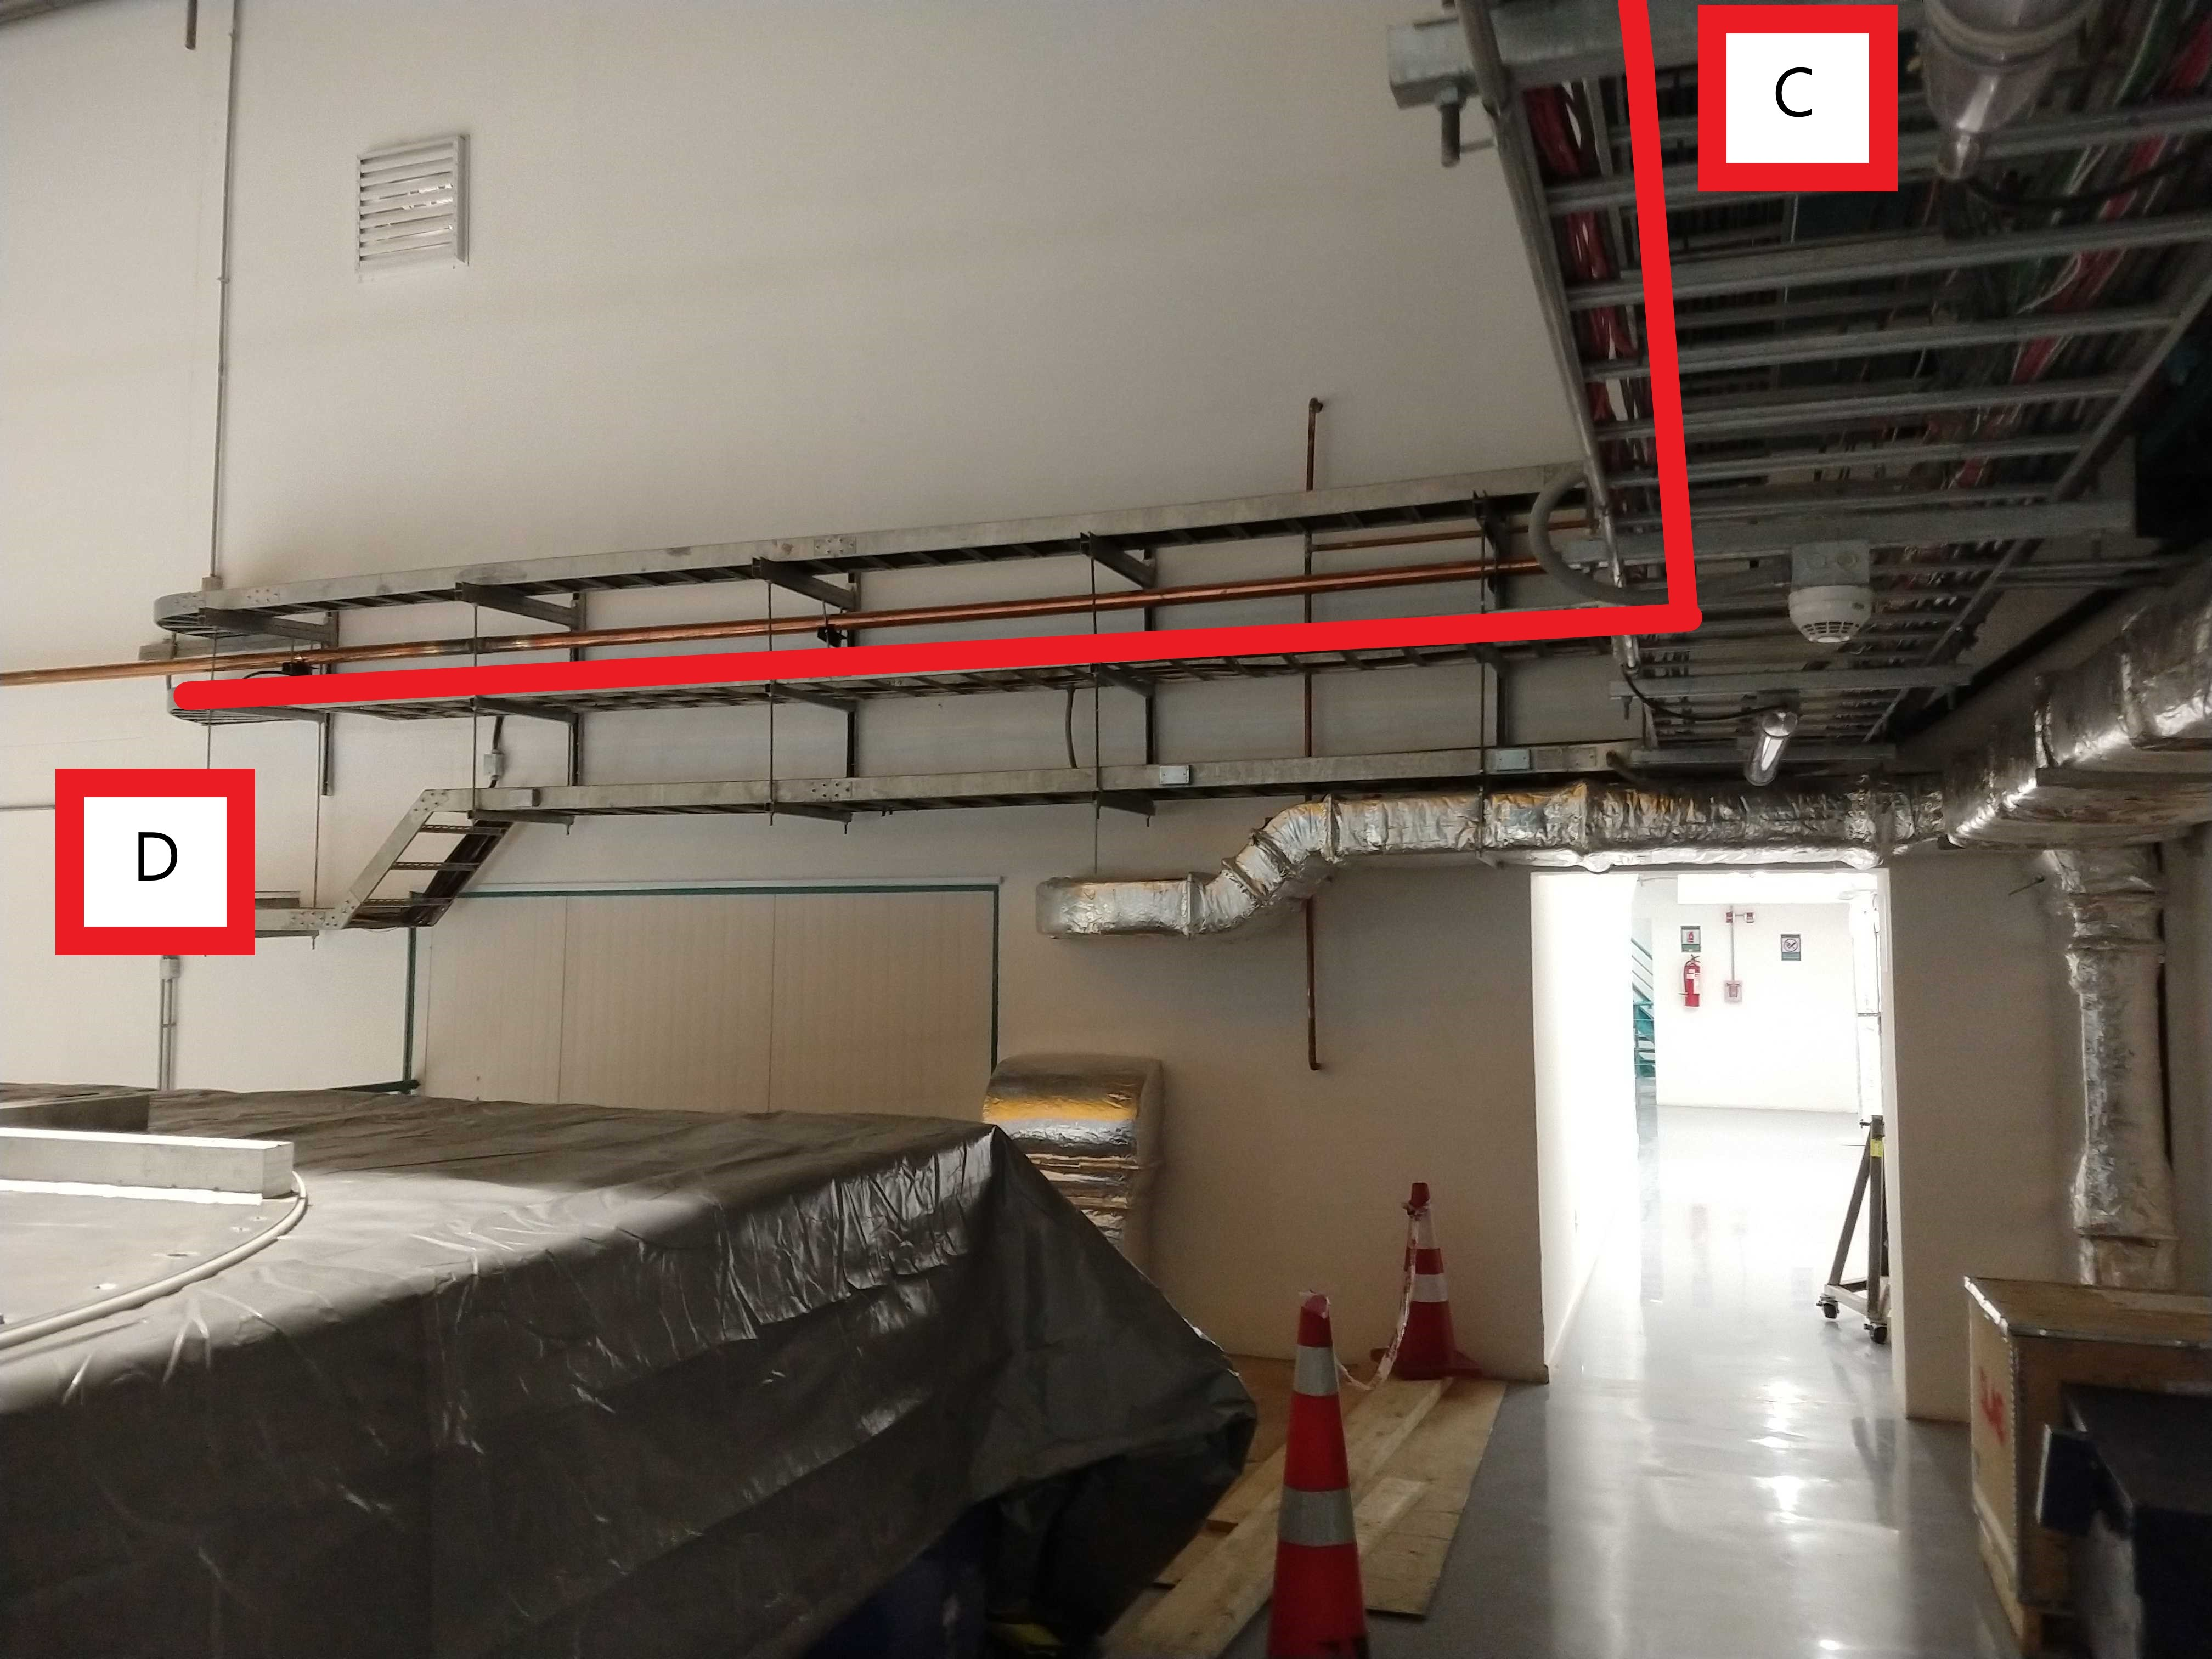
\includegraphics[width=10cm]{images/16.jpg}
    \caption*{The cable shows up again on the fourth floor of the main building and connects to the cable tray found on the same floor, the cable follows the path of the cable tray connecting to point D.}
  \end{figure}

\newpage

  \begin{figure}
    \centering
    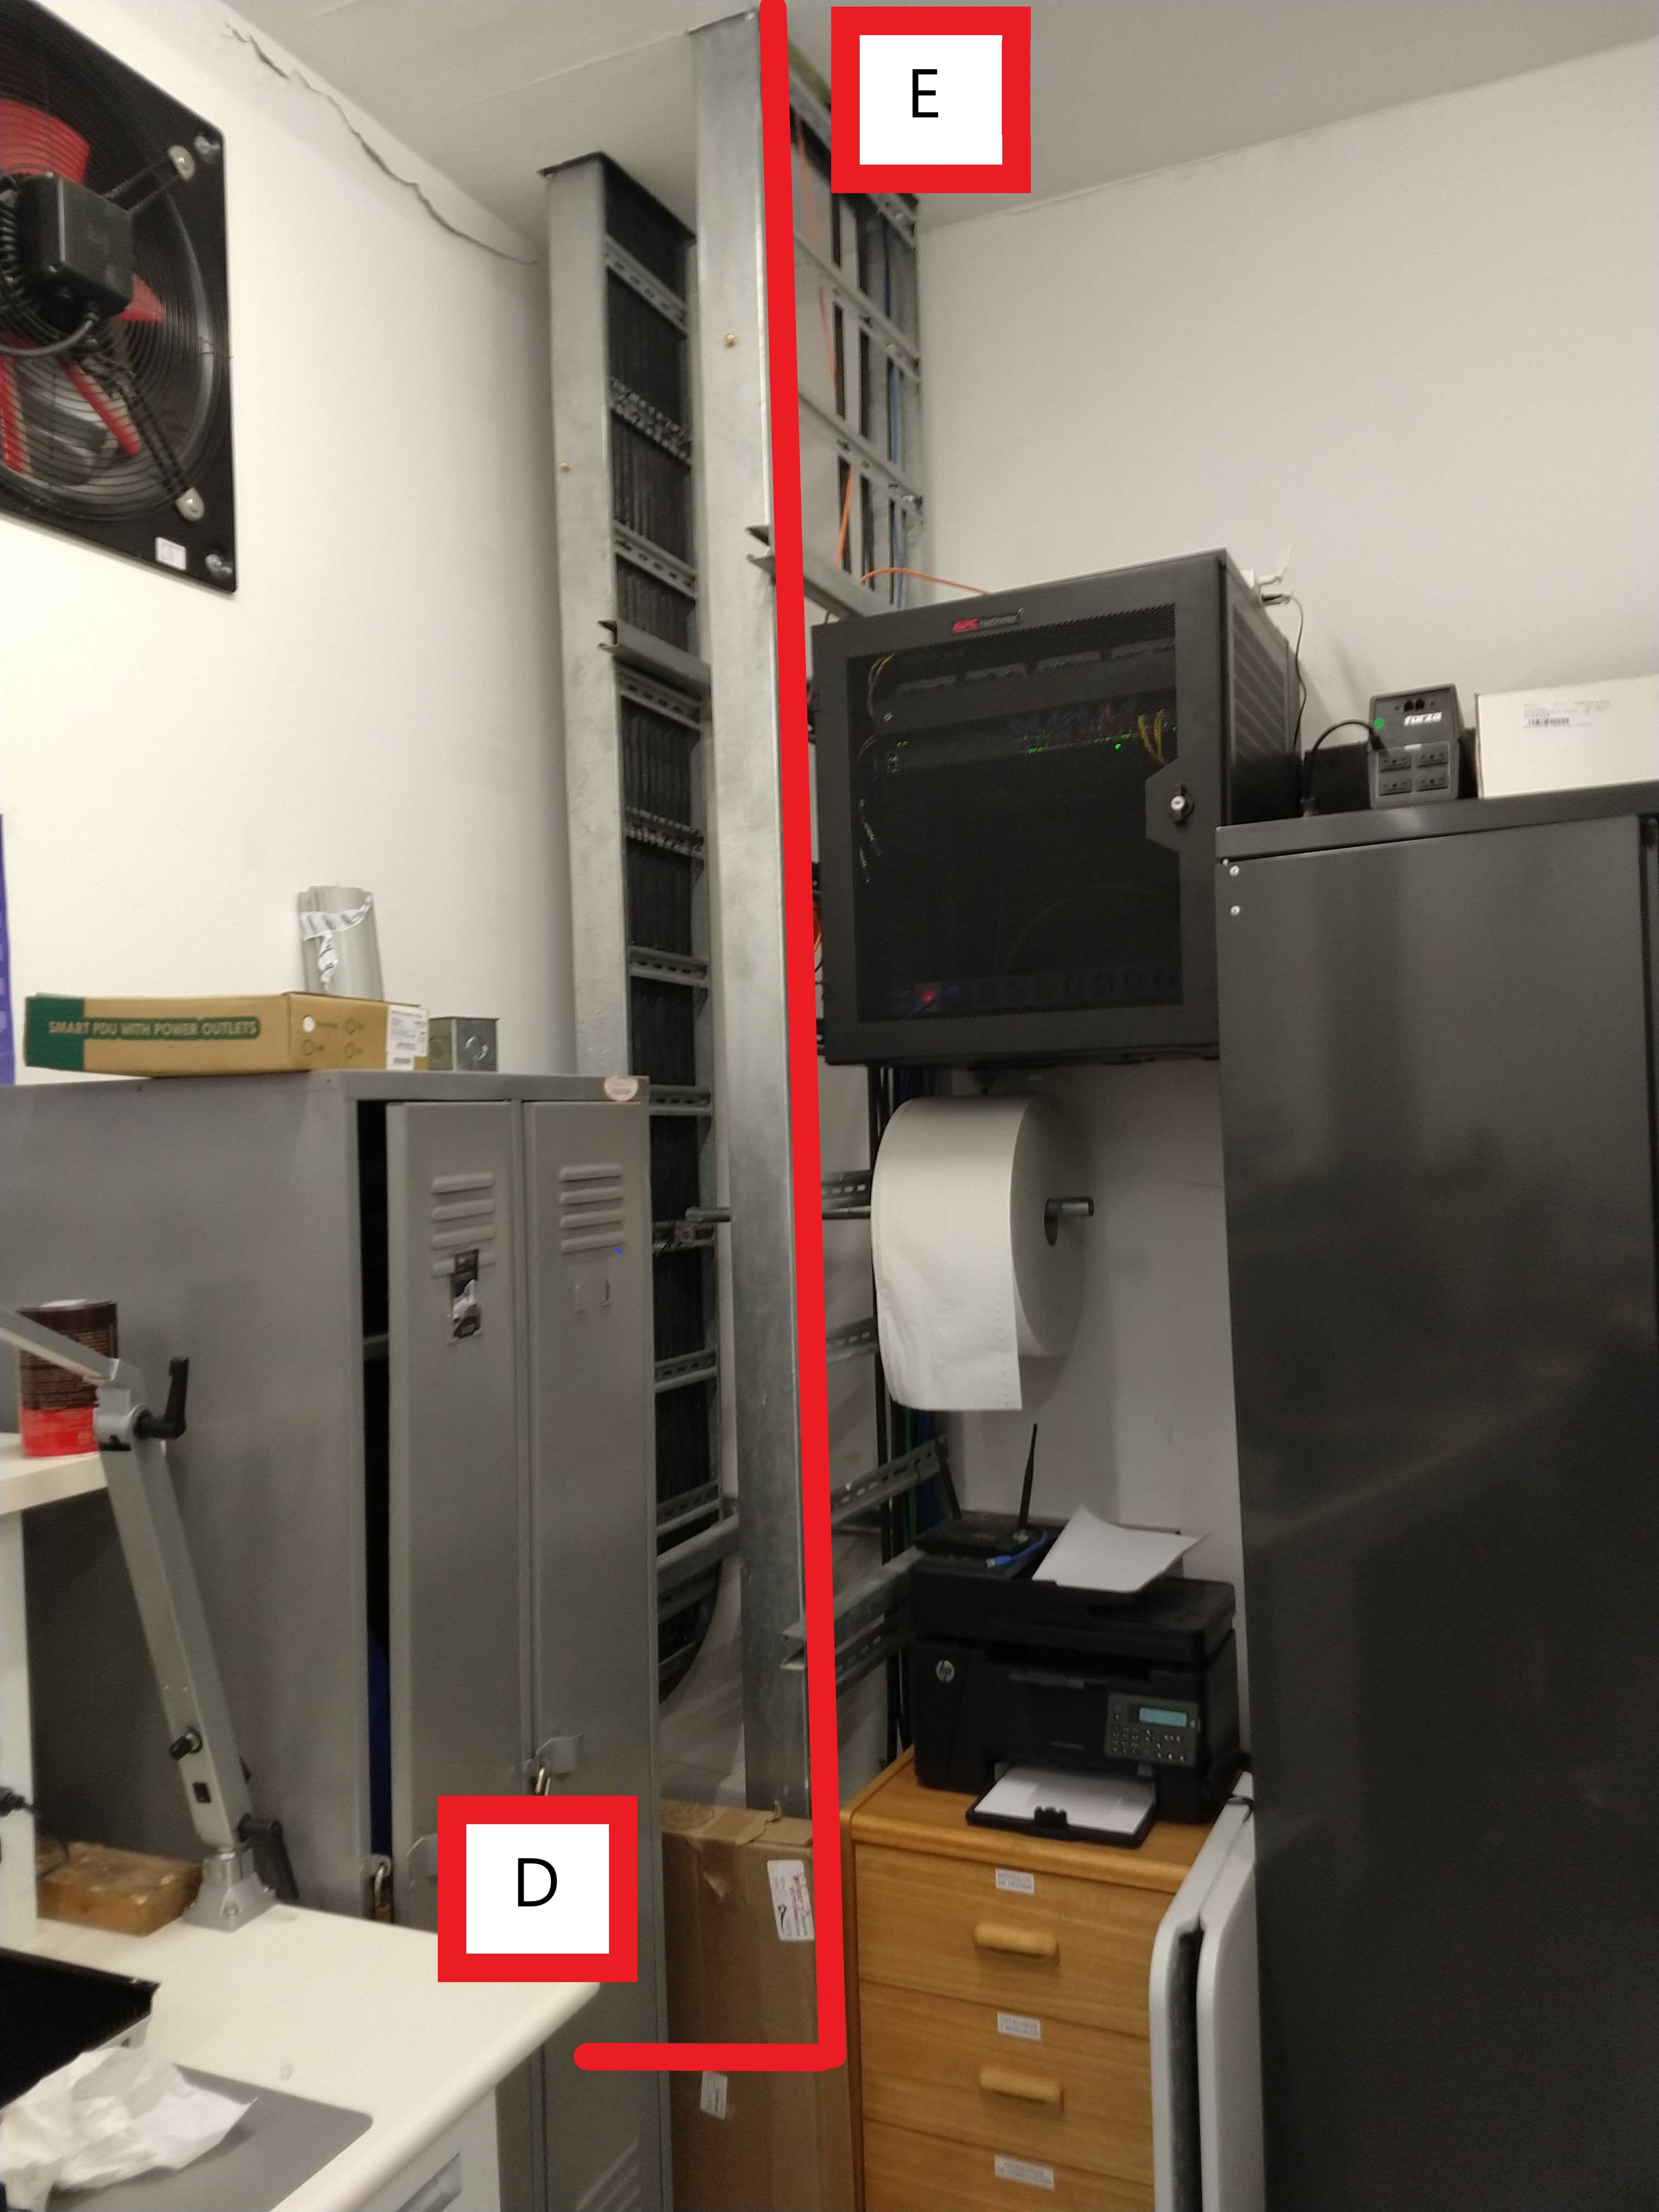
\includegraphics[width=6cm]{images/17.jpg}
  \end{figure}
  From here the cable goes inside the electronics laboratory room located on the fifth floor and follows the cable tray path to point E.
  \begin{figure}
    \centering
    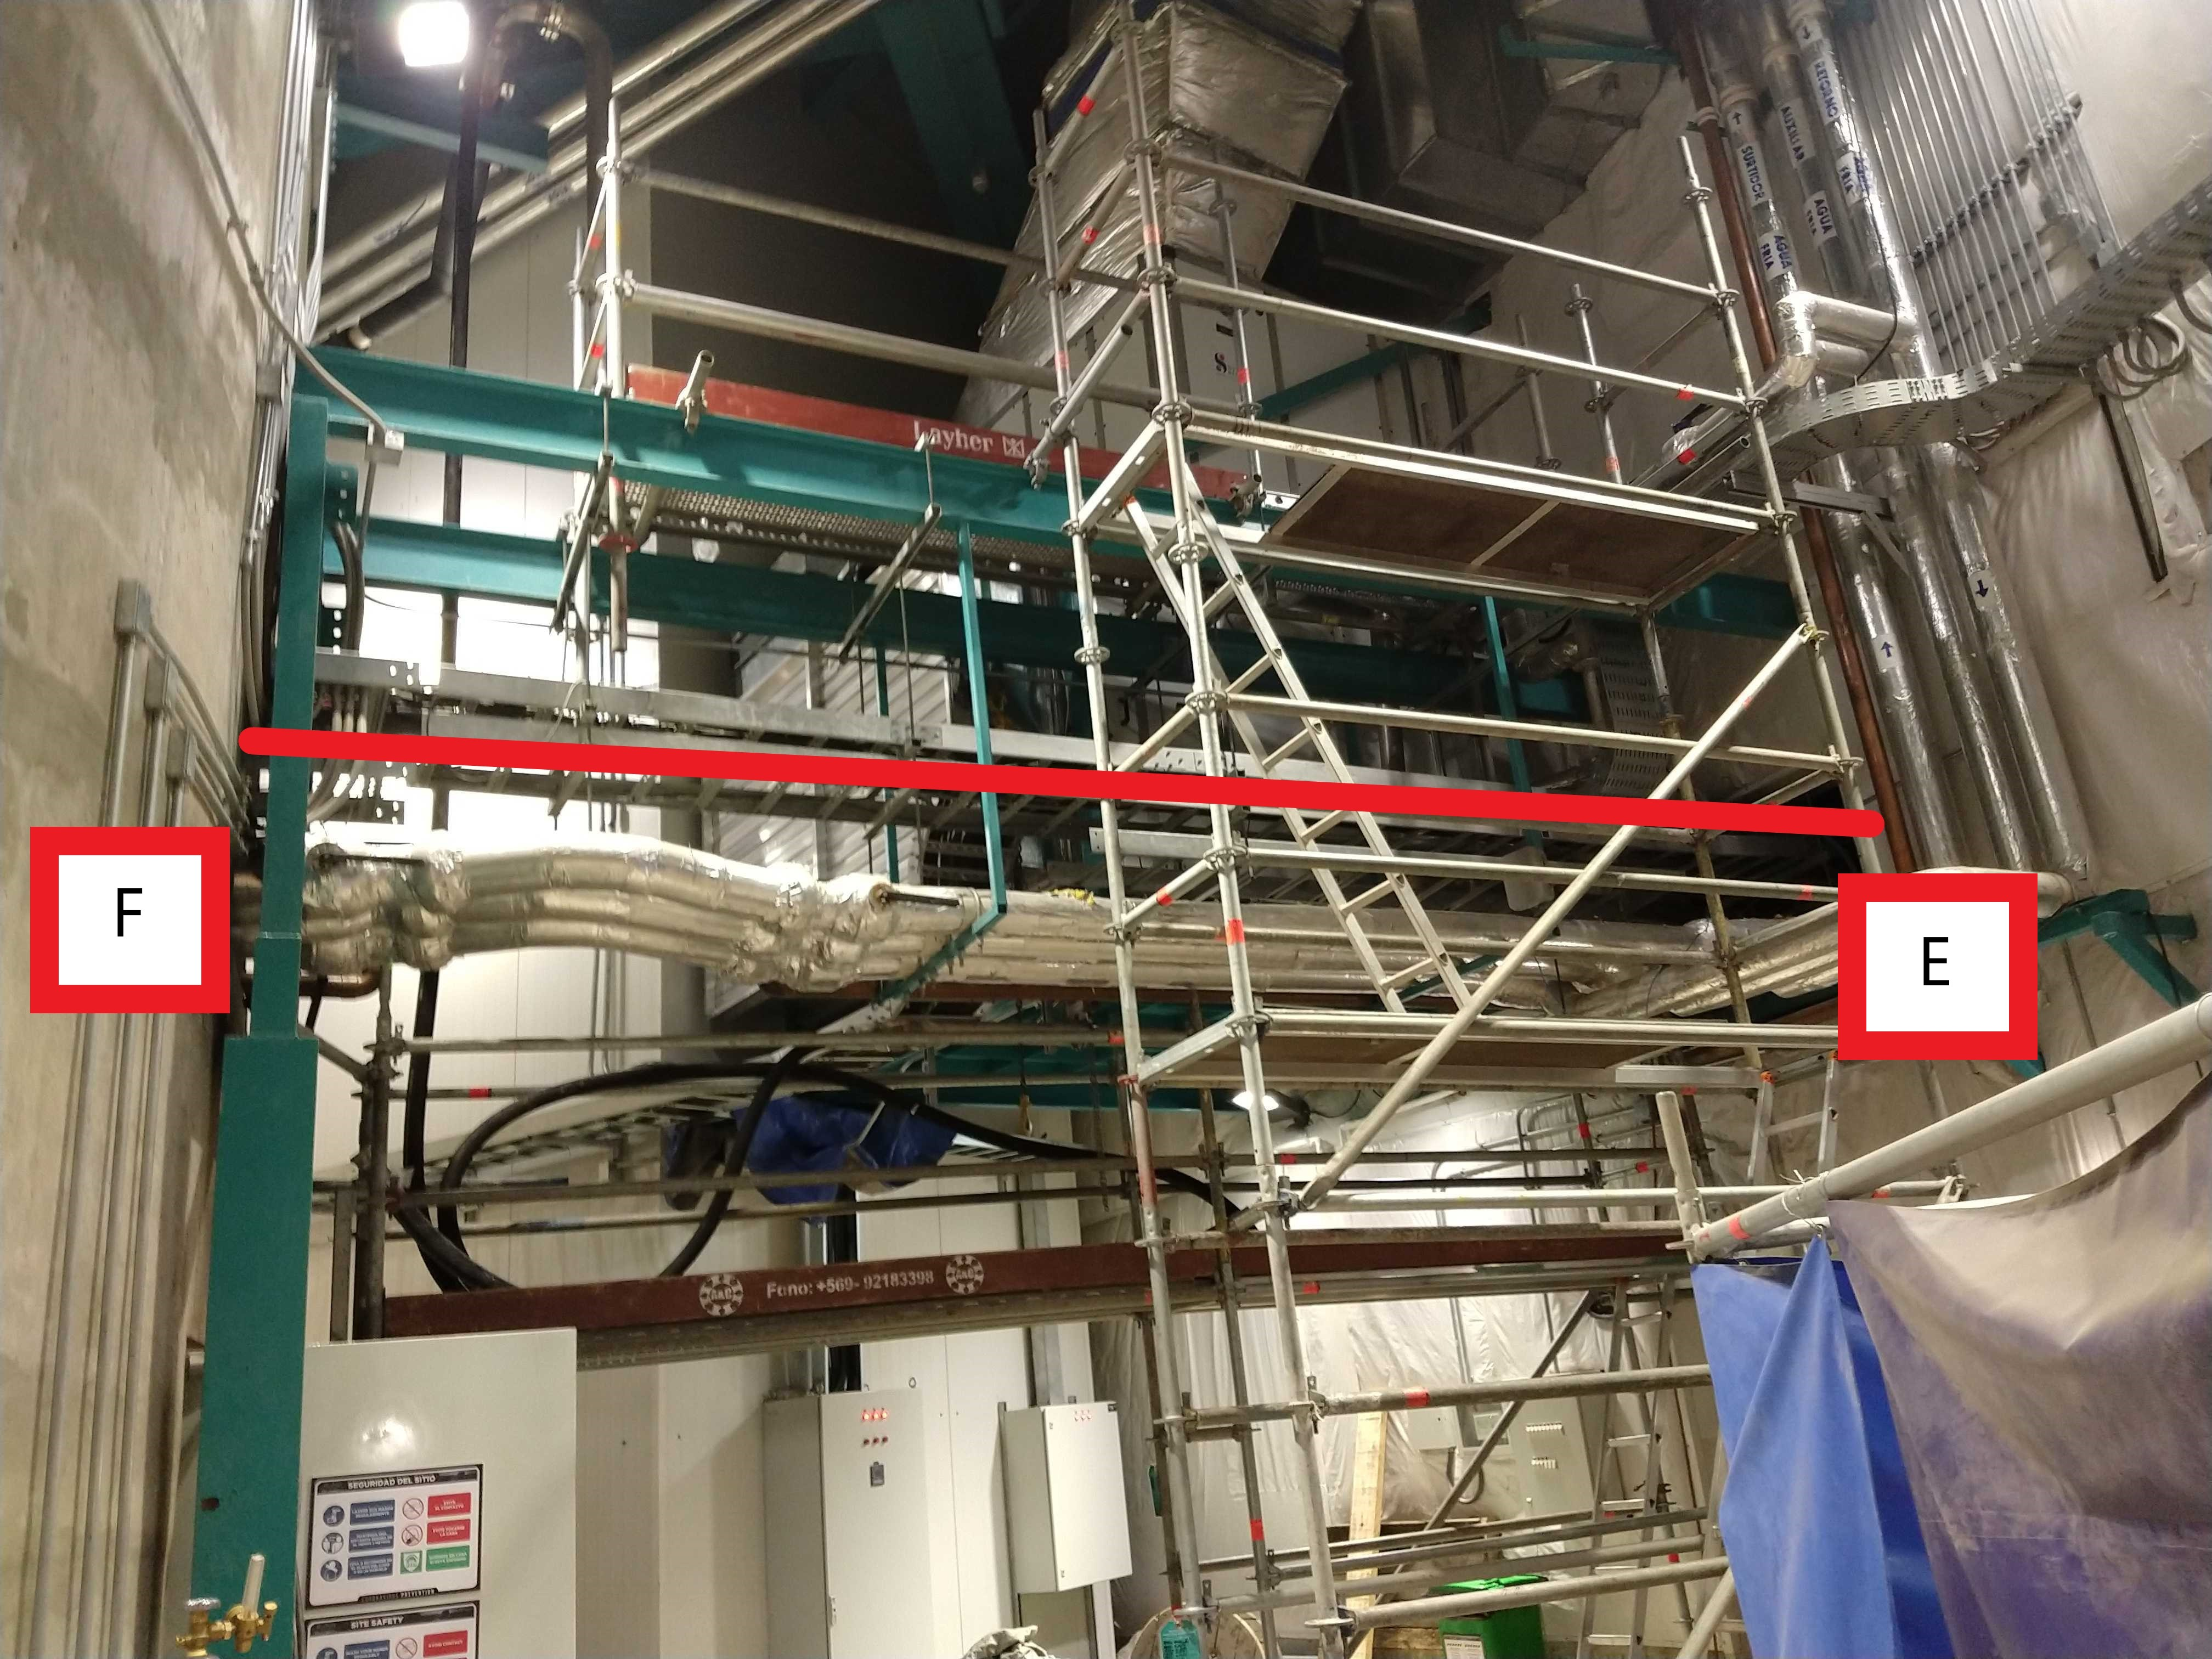
\includegraphics[width=10cm]{images/18.jpg}
    \caption*{The cable then runs in between the ceiling of the fifth floor and connects to the pier on point F of that same floor.}
  \end{figure}
  
\newpage

  \begin{figure}
    \centering
    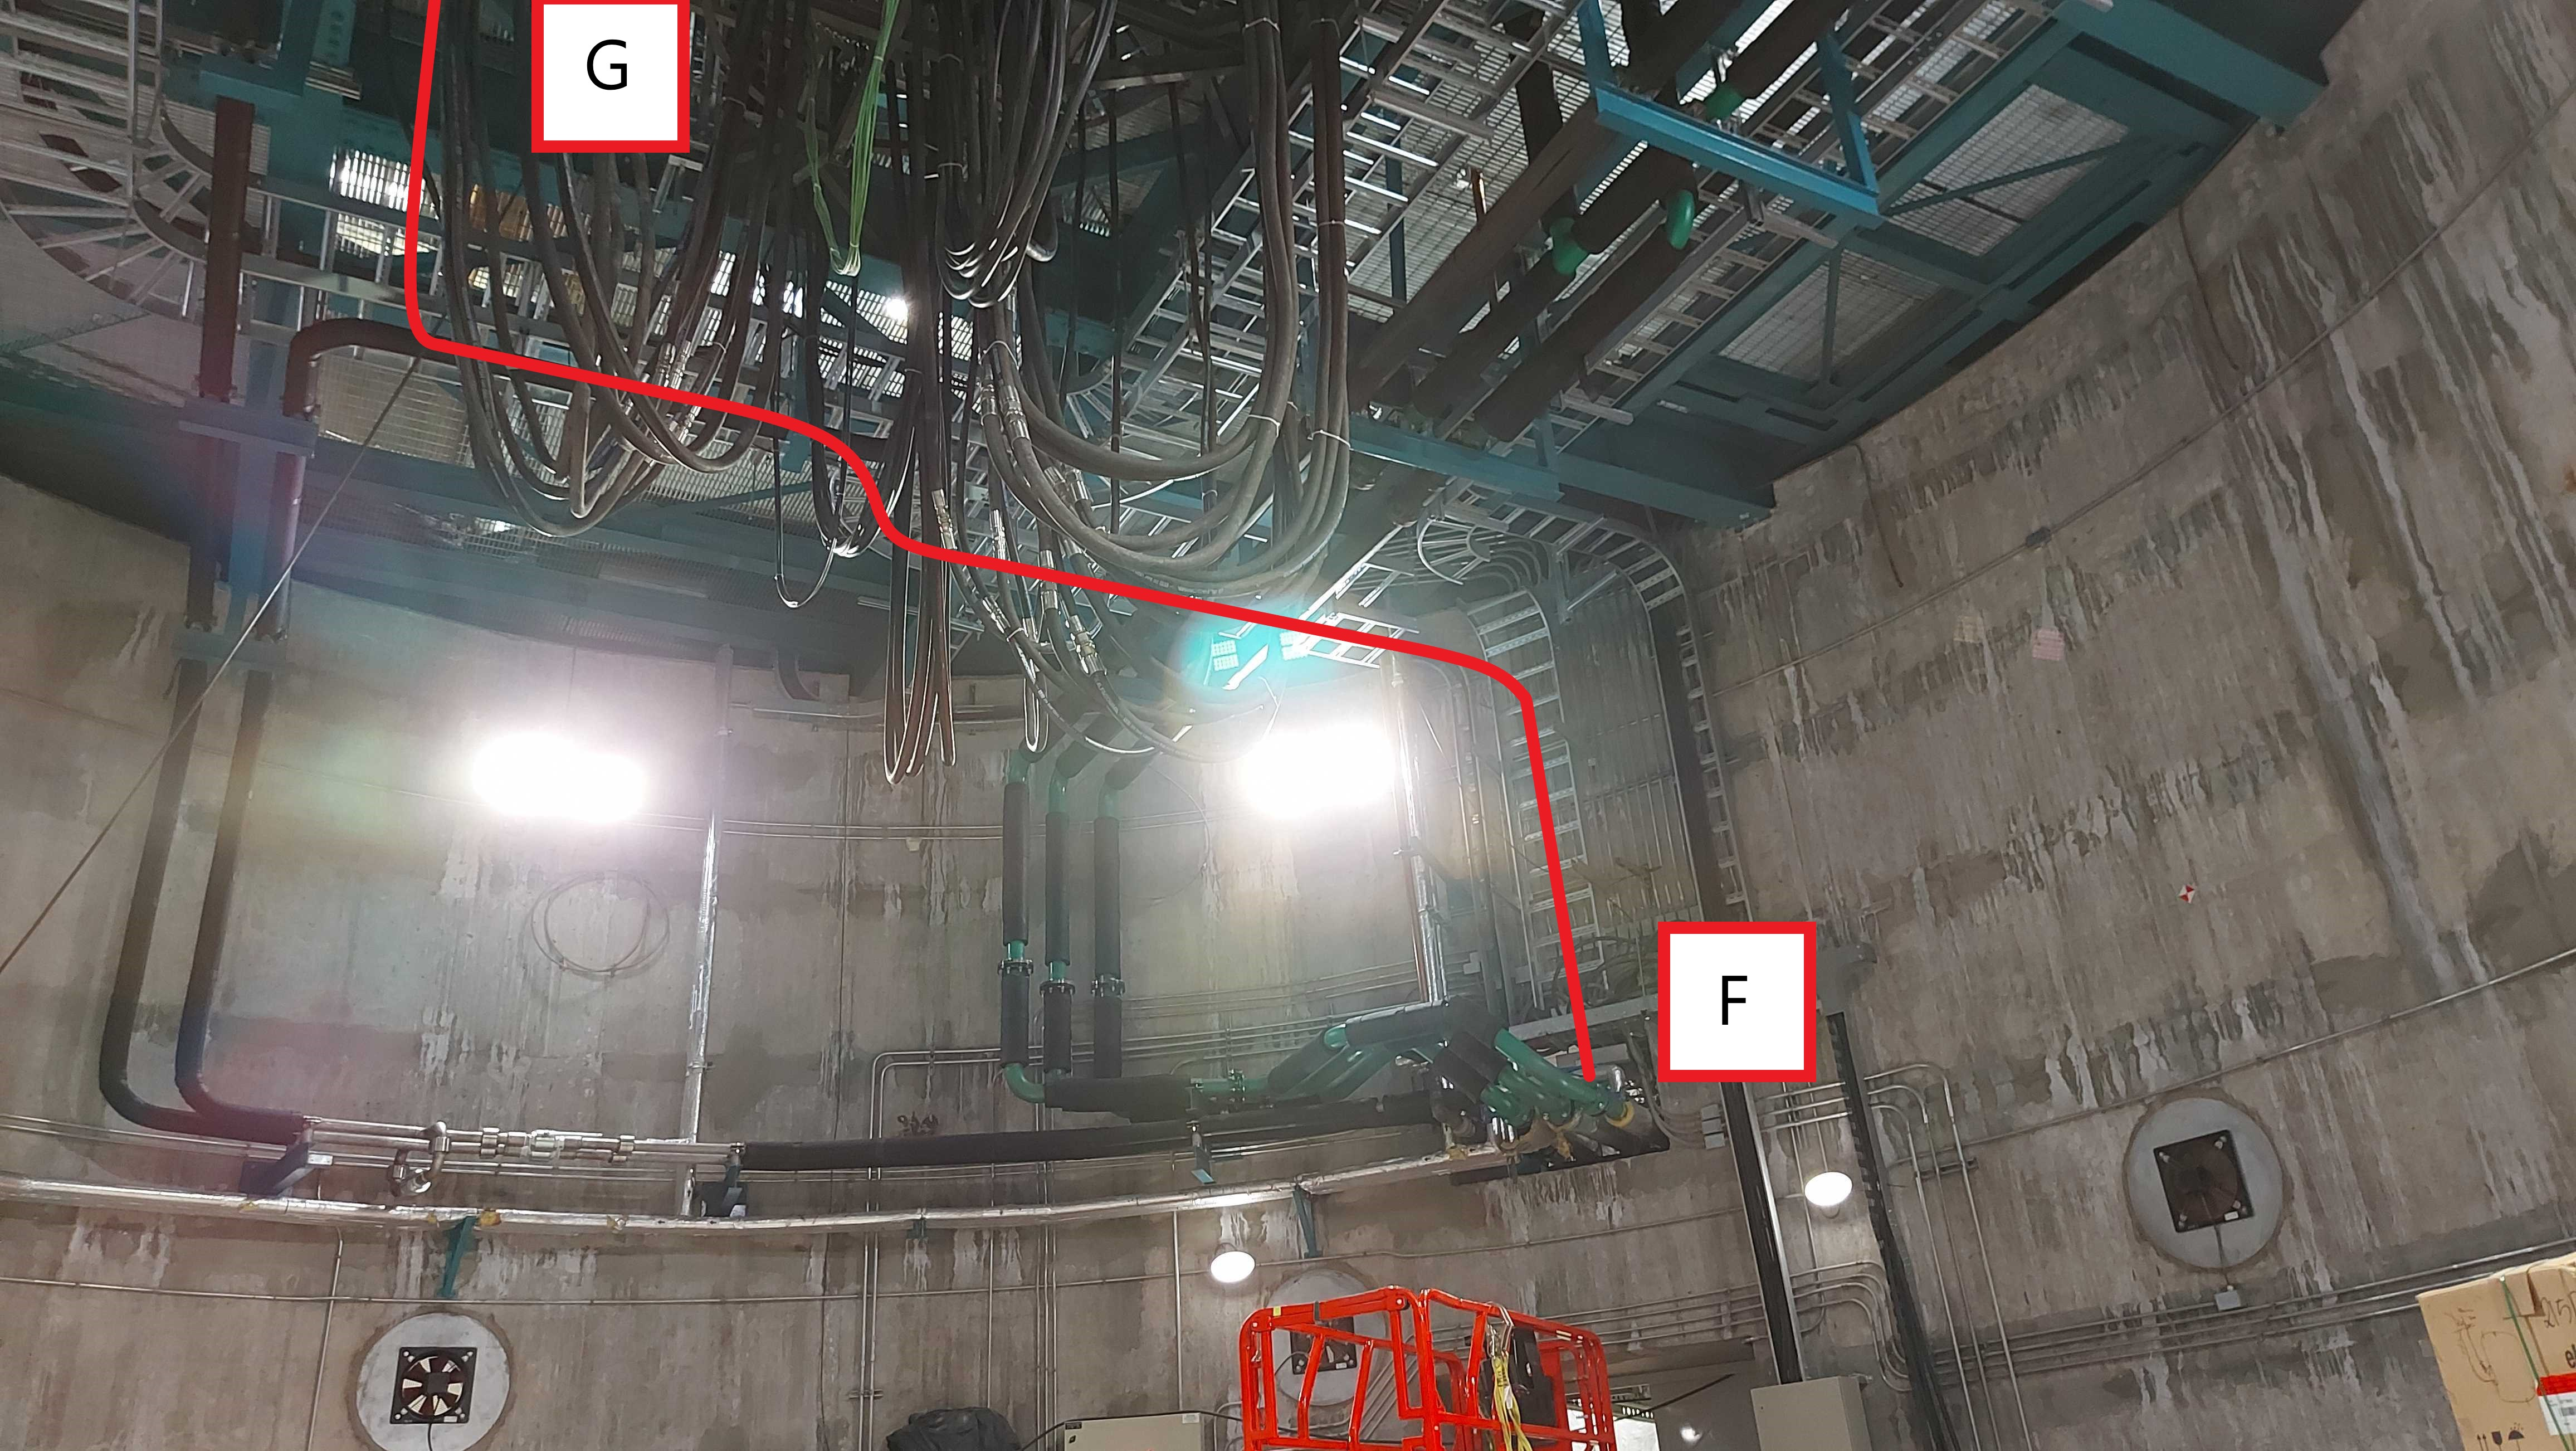
\includegraphics[width=15cm]{images/19-1.jpg}
    \caption*{The cable is routed inside the pier from position F to a specifically built cable tray extending to point G.}
  \end{figure}
  \begin{figure}
    \centering
    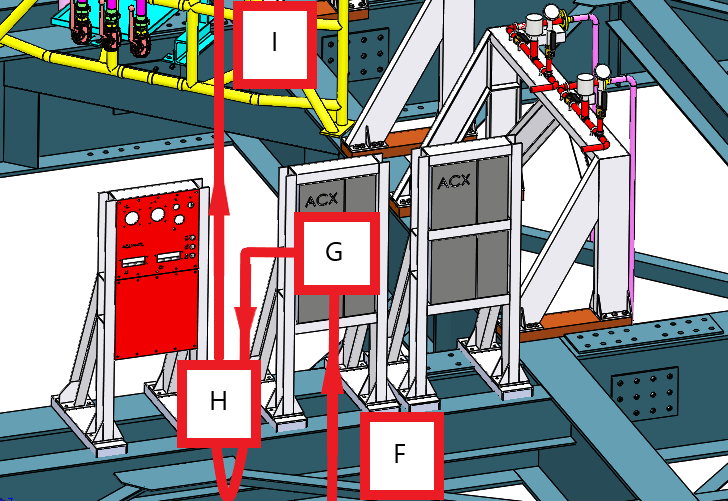
\includegraphics[width=10cm]{images/21-1.png}
    \caption*{The cable extends from point F and connects to the optical terminal located at position G. The cable later descends to point H and comes back up through the azimuth drape to point I.}
  \end{figure}

\newpage

  \begin{figure}
    \centering
    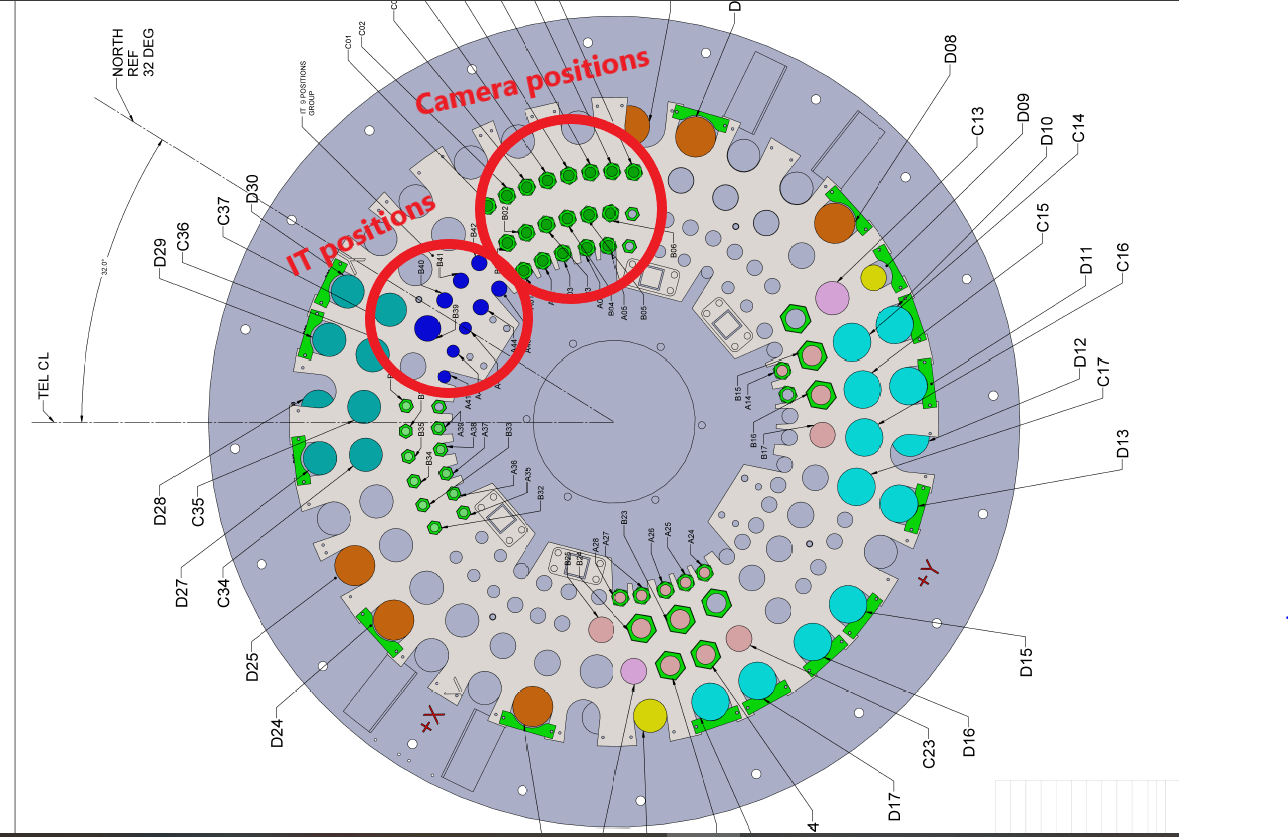
\includegraphics[width=10cm]{images/22.png}
    \caption*{The following image illustrates the various positions assigned in the azimuth drape.The green-colored circles are reserved positions for the camera fibers and the blue-colored circles are the positions reserved for IT future cable installations.}
  \end{figure}
  \begin{figure}
    \centering
    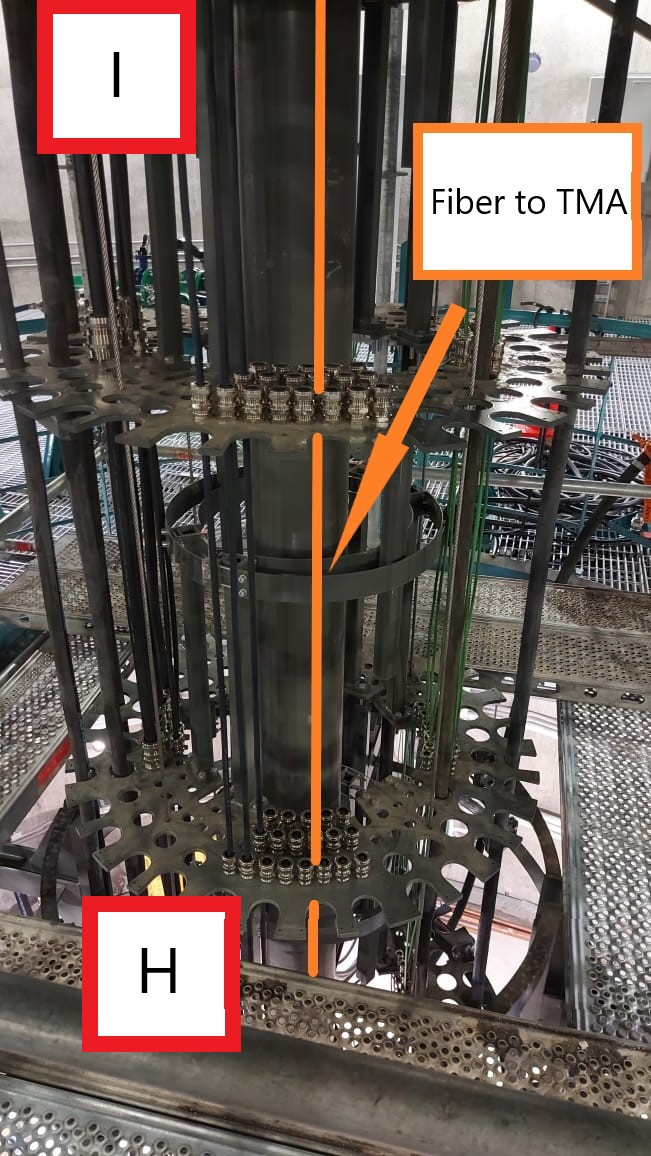
\includegraphics[width=5cm]{images/22-1.jpg}
    \caption*{The cable travels along with the azimuth drape from point H towards the top of the 6th floor at position I.}
  \end{figure}

\newpage

  \begin{figure}
    \centering
    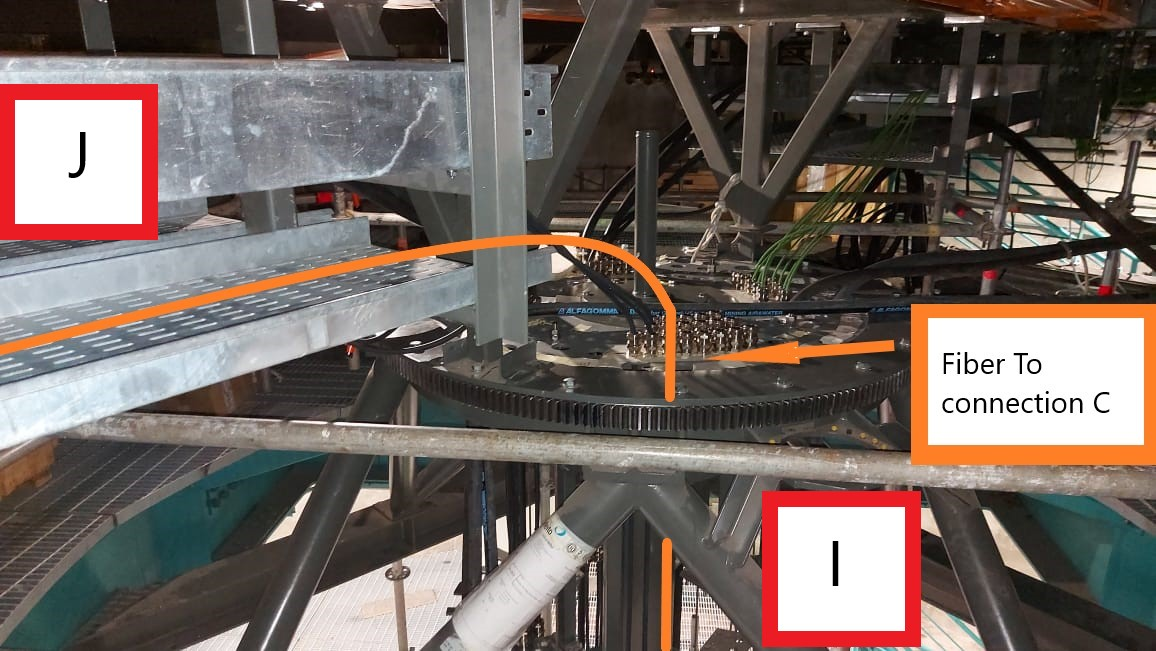
\includegraphics[width=10cm]{images/23.jpg}
    \caption*{From the position I, the cable is routed up the ladder position to point J.}
  \end{figure}
  \begin{figure}
    \centering
    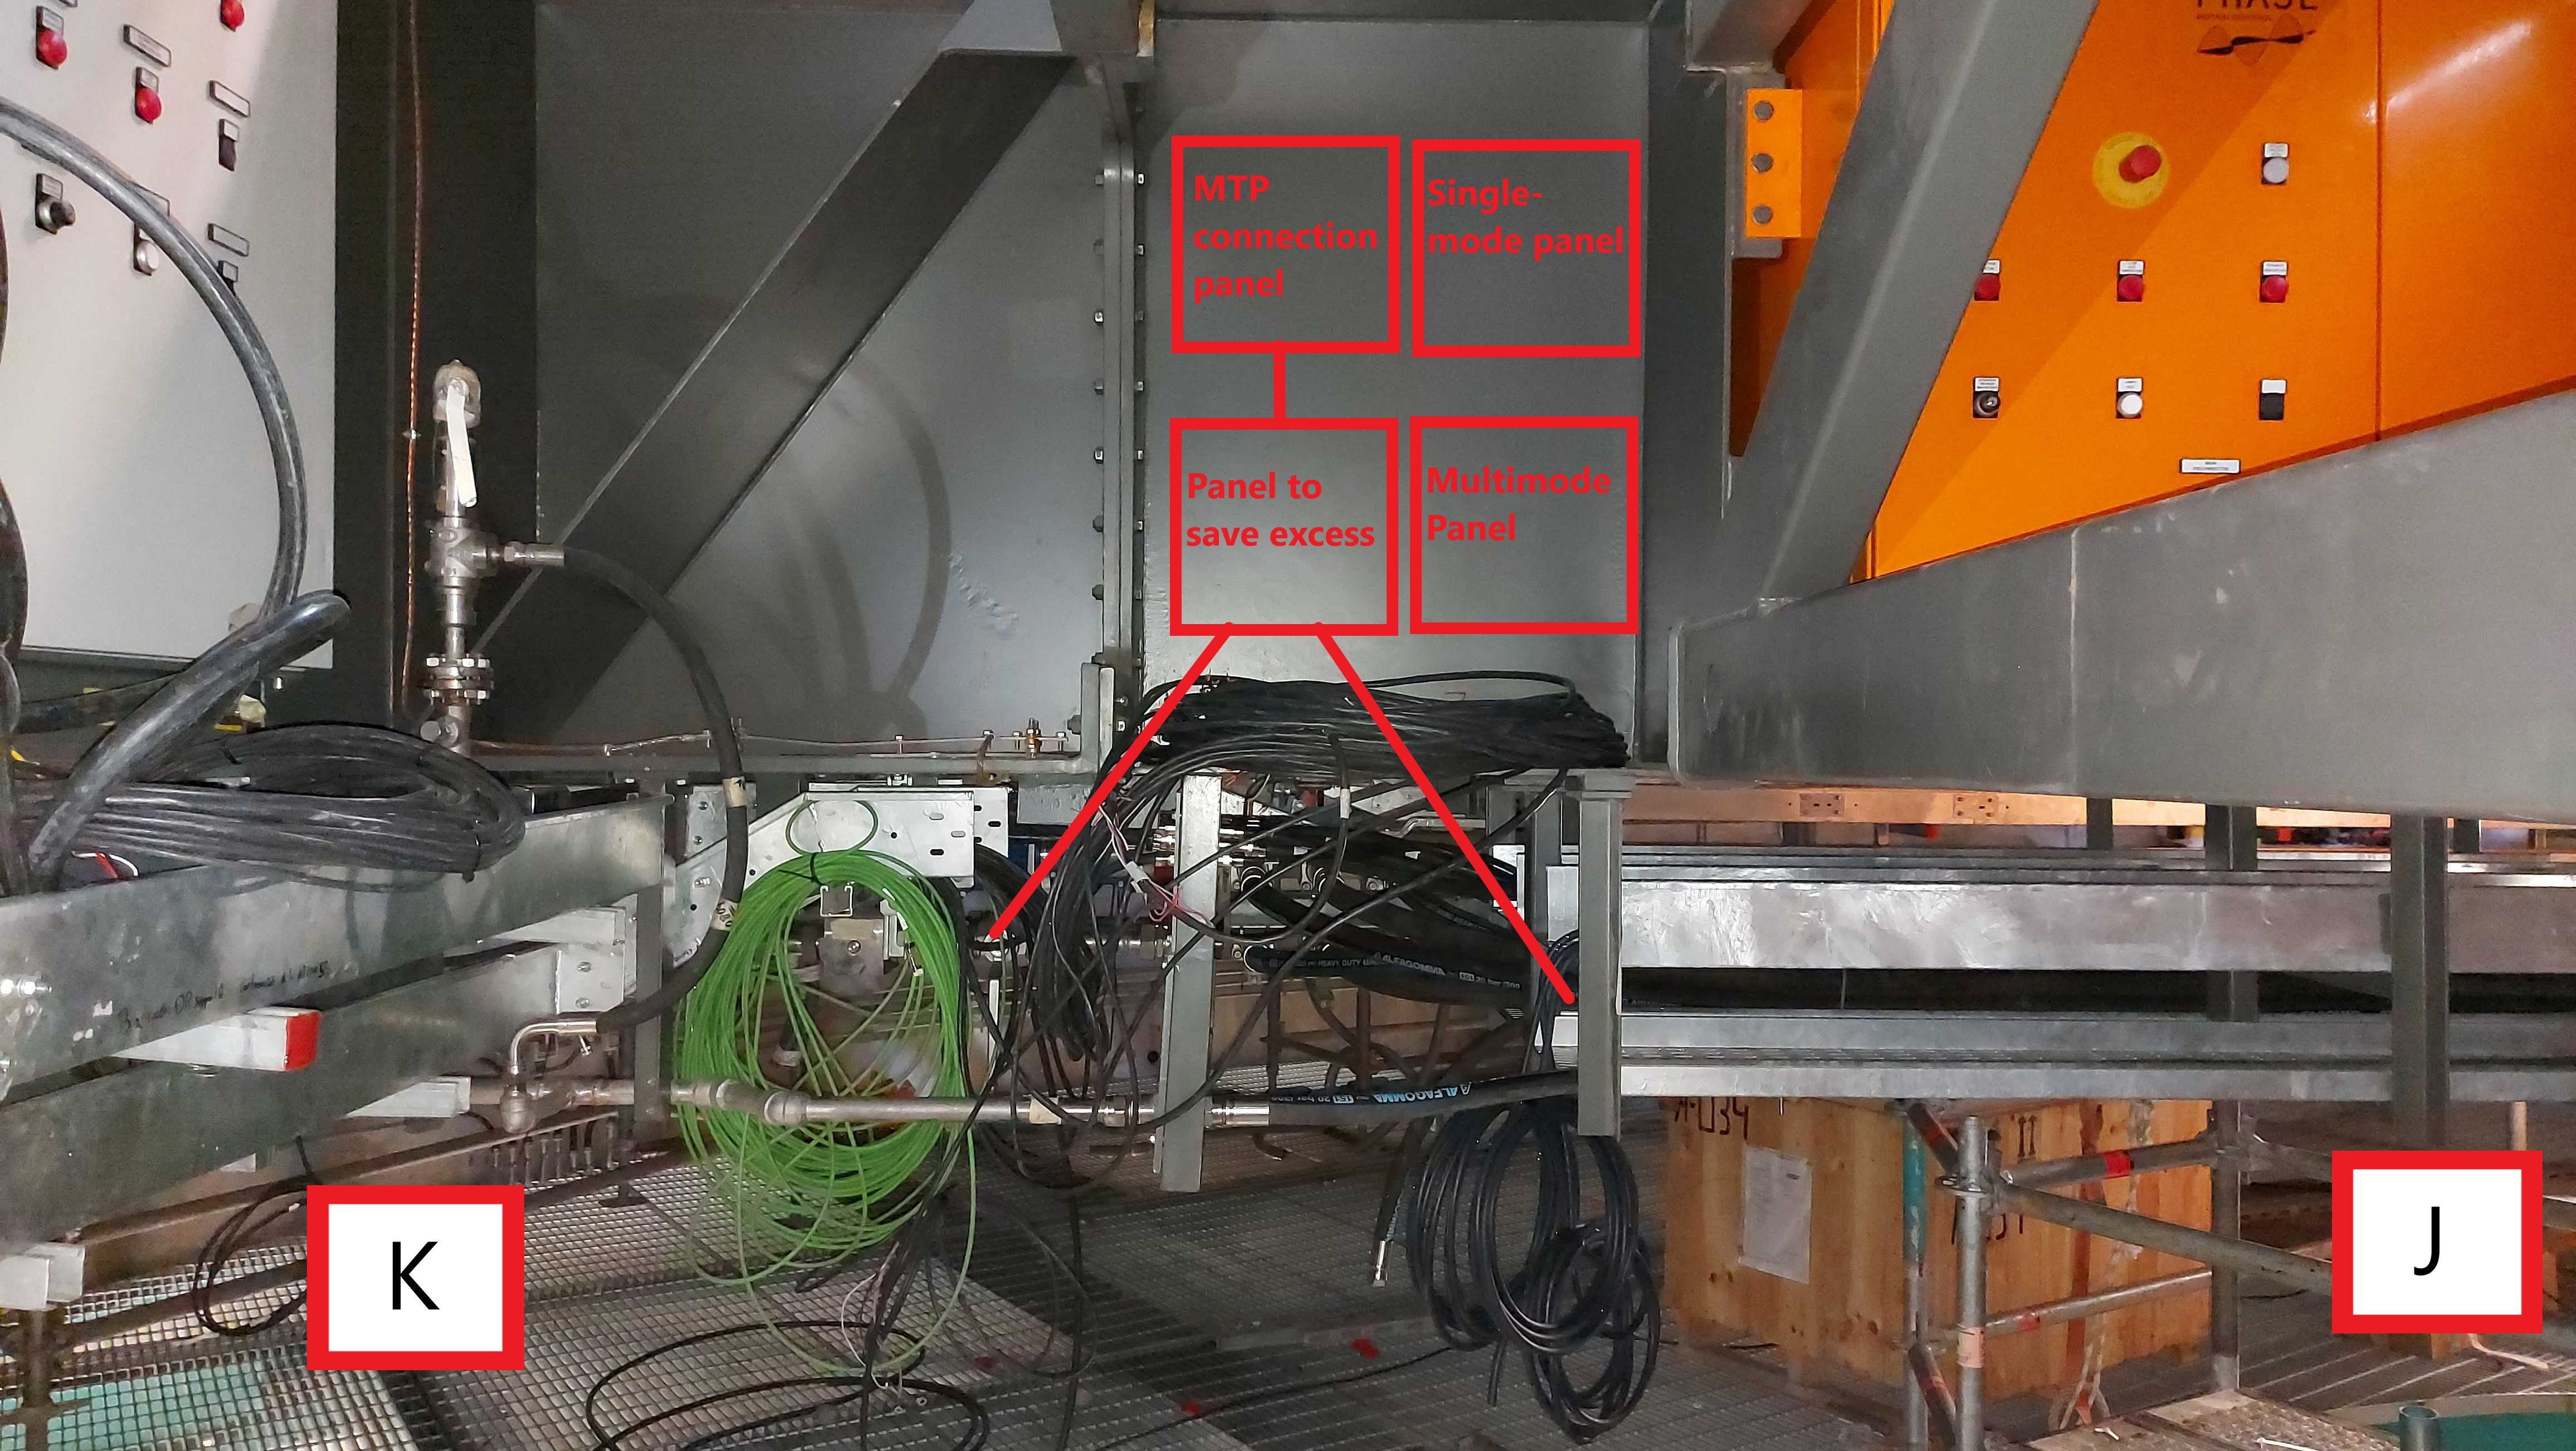
\includegraphics[width=10cm]{images/24.jpg}
    \caption*{The cable then connects from point J to the optical end that will later be constructed in the area illustrated above. From here on, the cable is routed from the optical terminal and travels along the ladder to point K.}
  \end{figure}

\newpage

  \begin{figure}
    \centering
    \begin{subfigure}{0.60\textwidth}
      \centering
      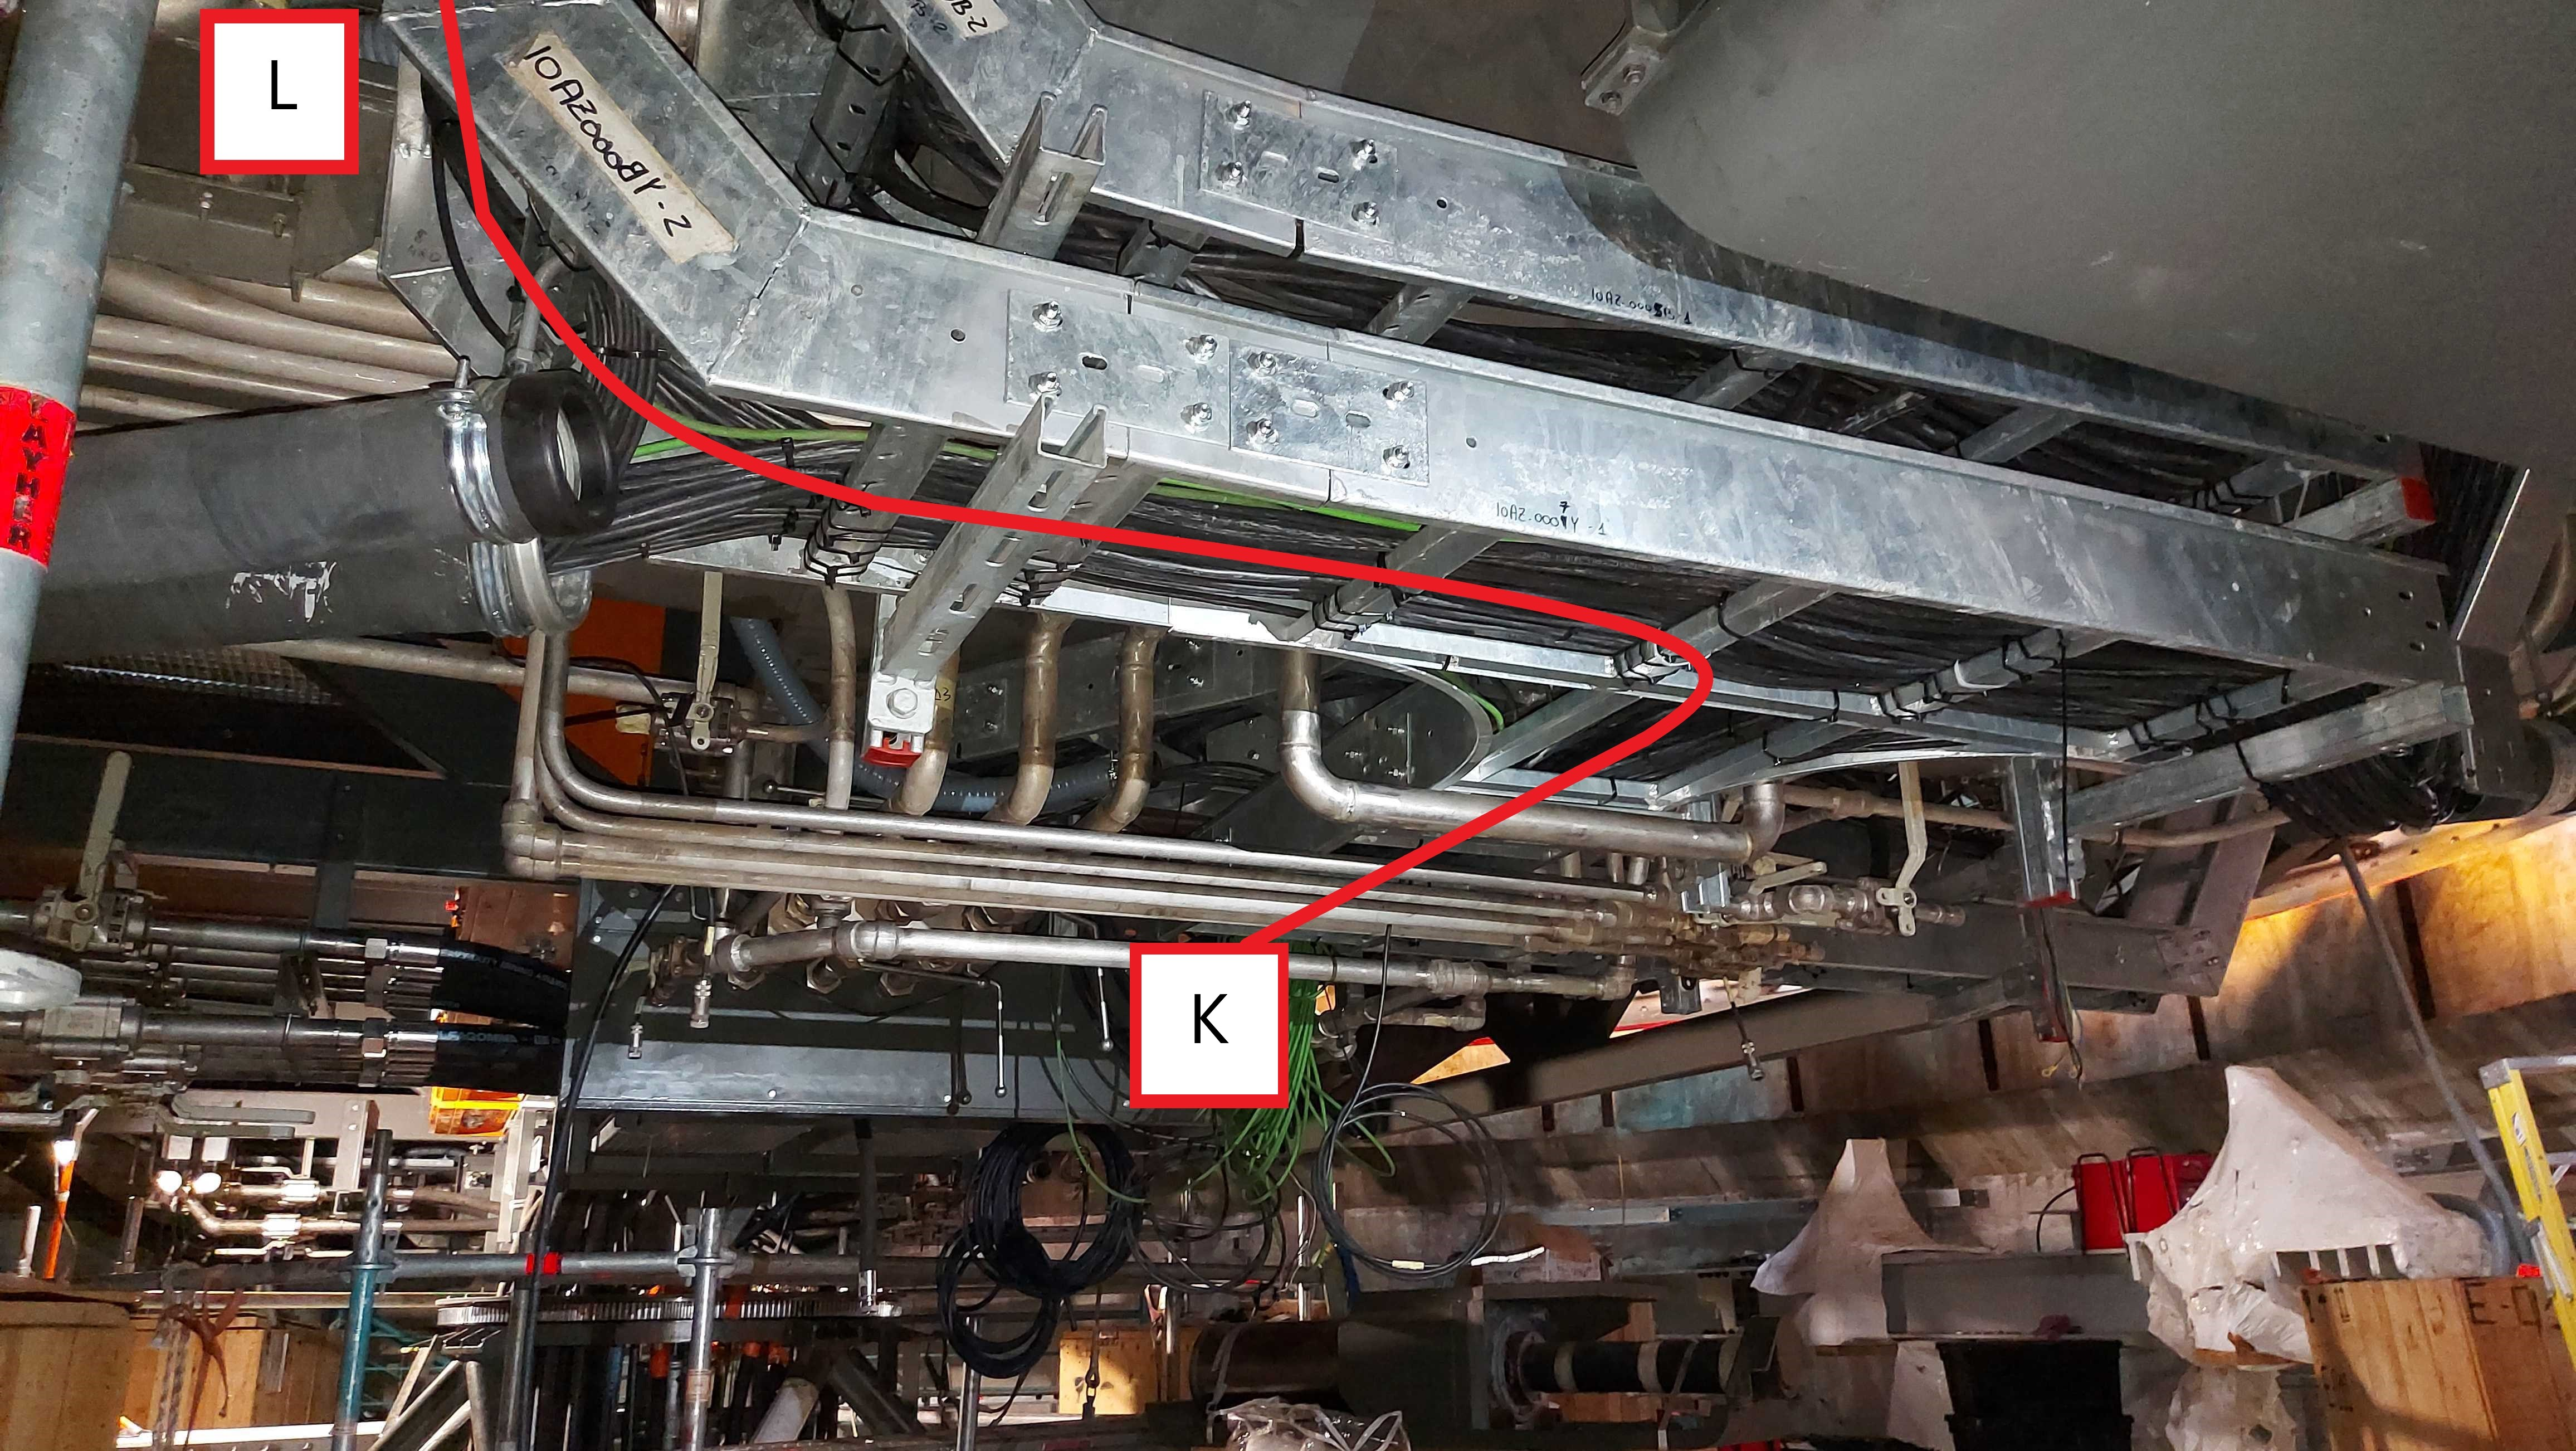
\includegraphics[width=\textwidth]{images/25.jpg}
    \end{subfigure}
    \hfill
    \begin{subfigure}{0.40\textwidth}
      \centering
      \includegraphics[width=\textwidth]{images/26-.png}
    \end{subfigure}
    \caption*{From position K, the cable follows the cable tray path to point L extending to the floor above.}
  \end{figure}

\newpage

  \begin{figure}
    \centering
    \begin{subfigure}{0.40\textwidth}
      \centering
      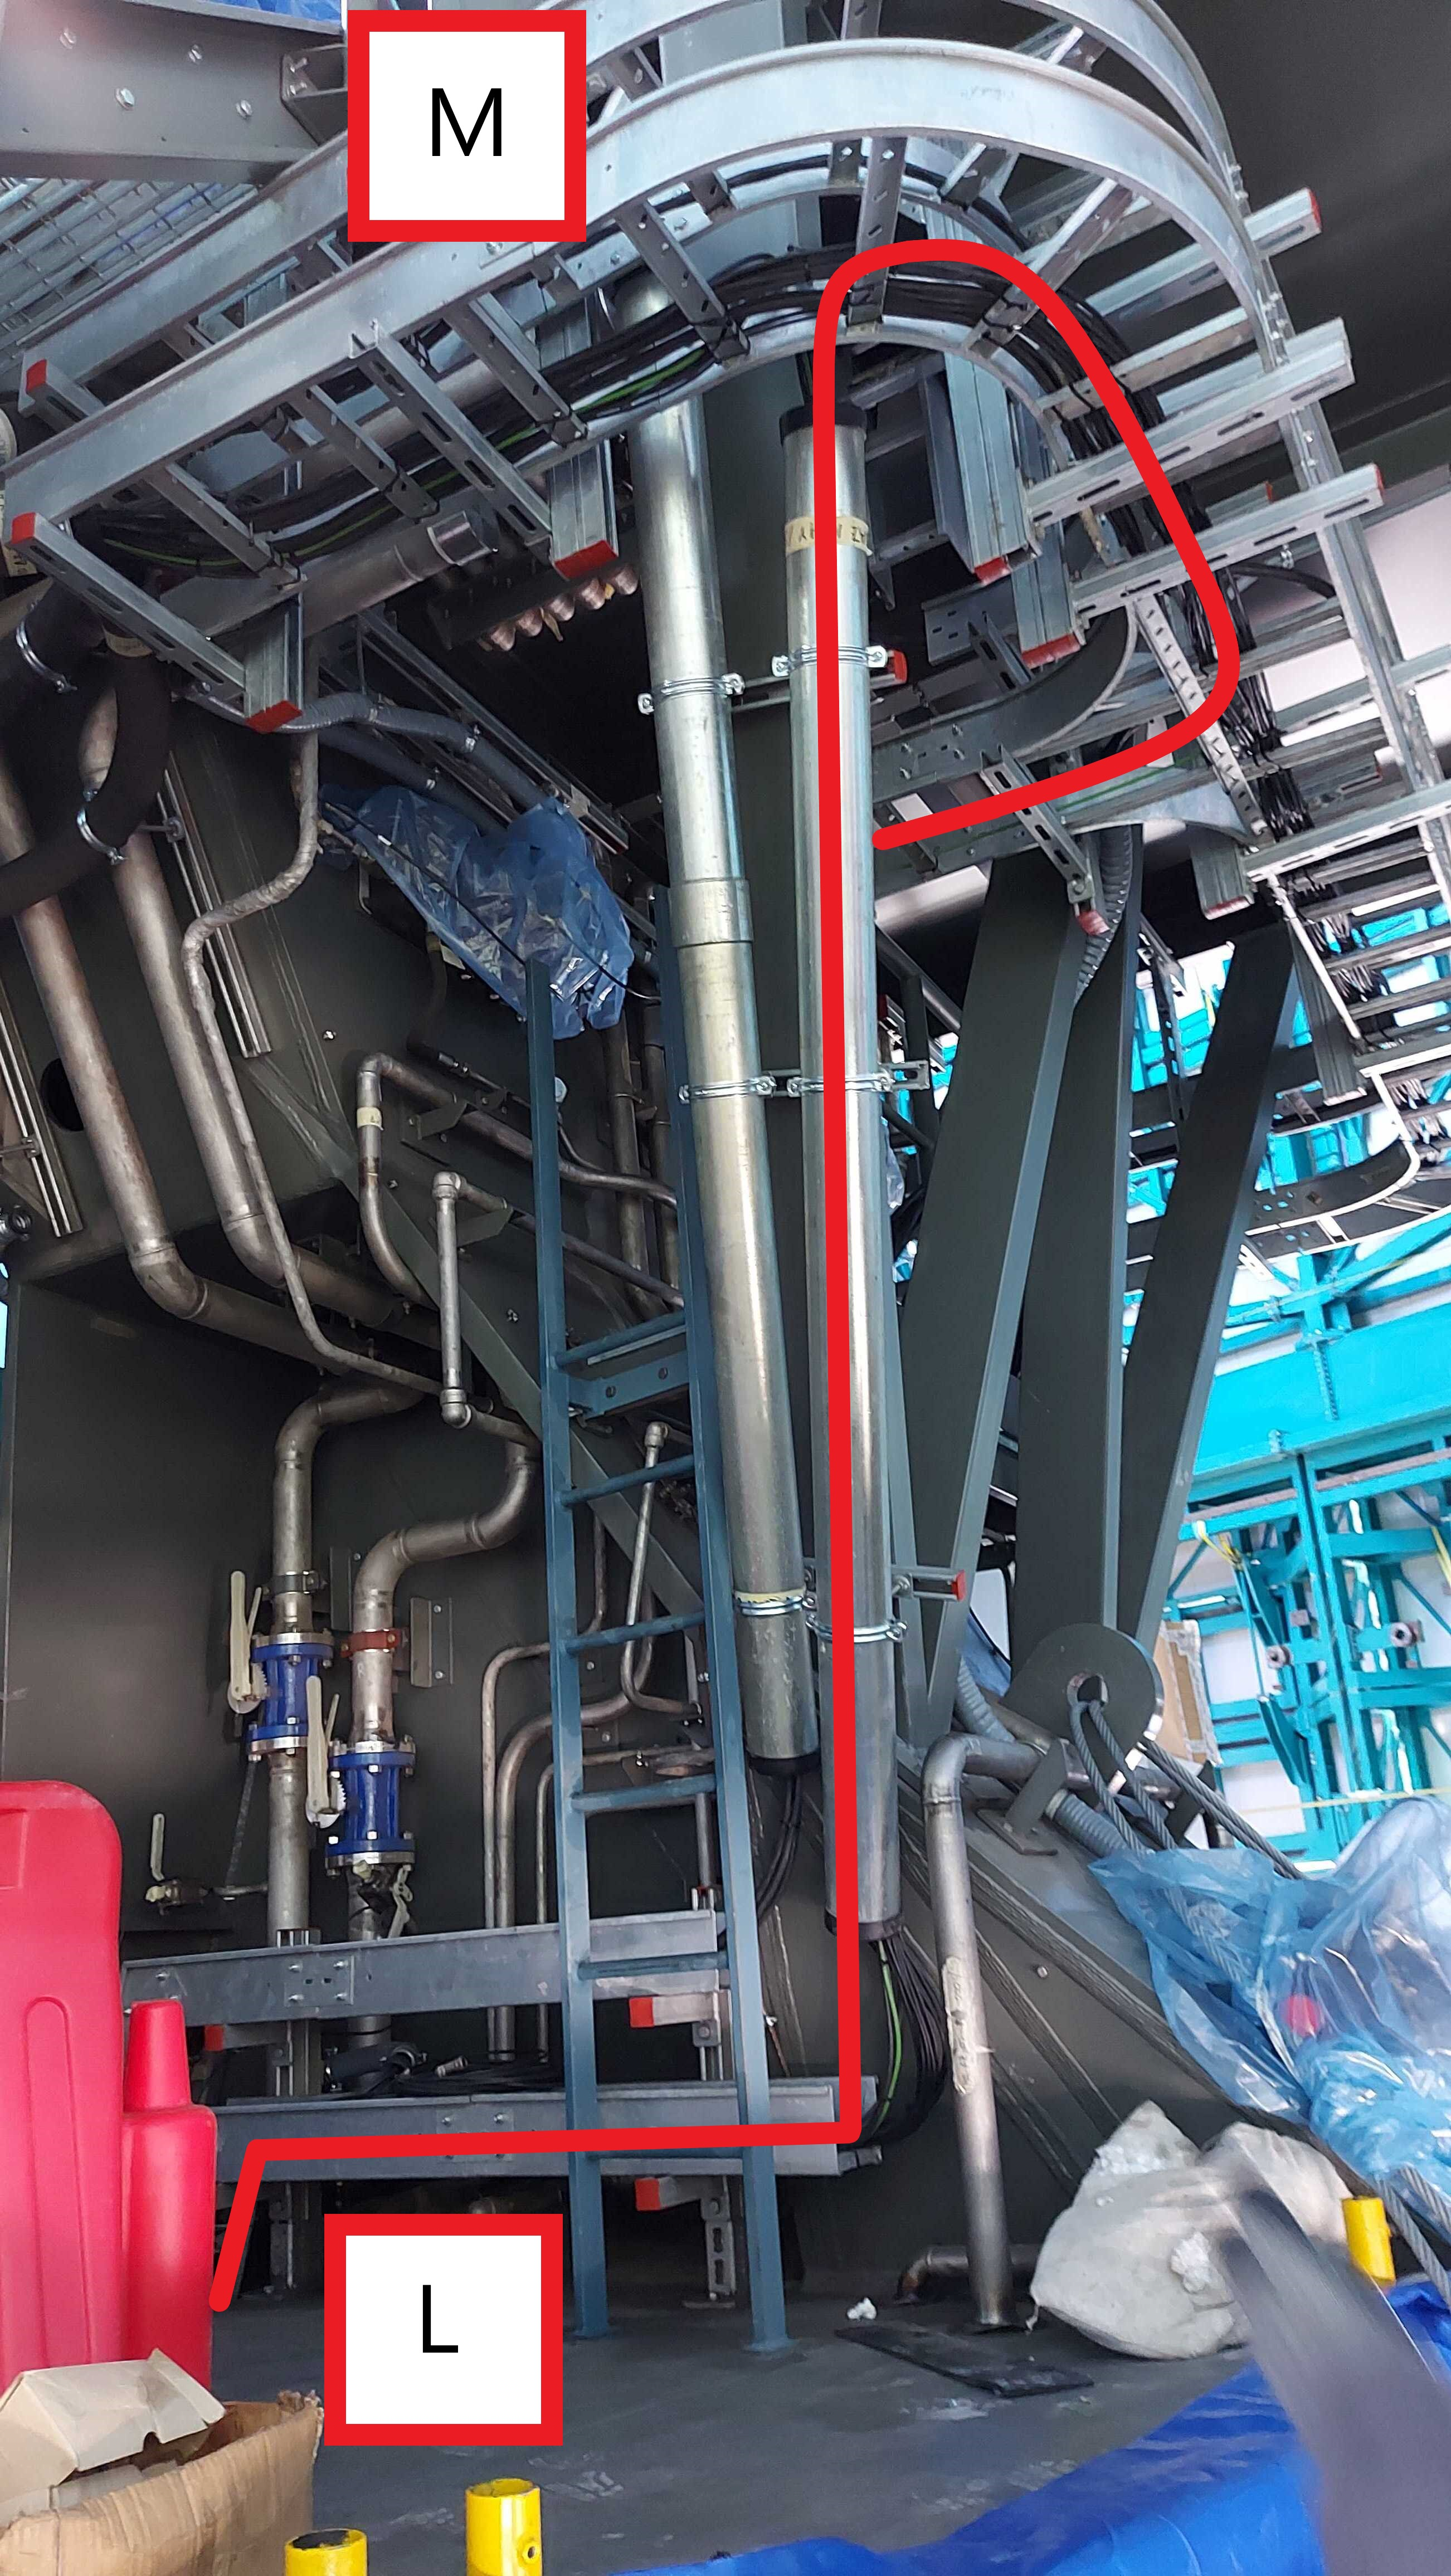
\includegraphics[width=\textwidth]{images/27.jpg}
    \end{subfigure}
    \hfill
    \begin{subfigure}{0.40\textwidth}
      \centering
      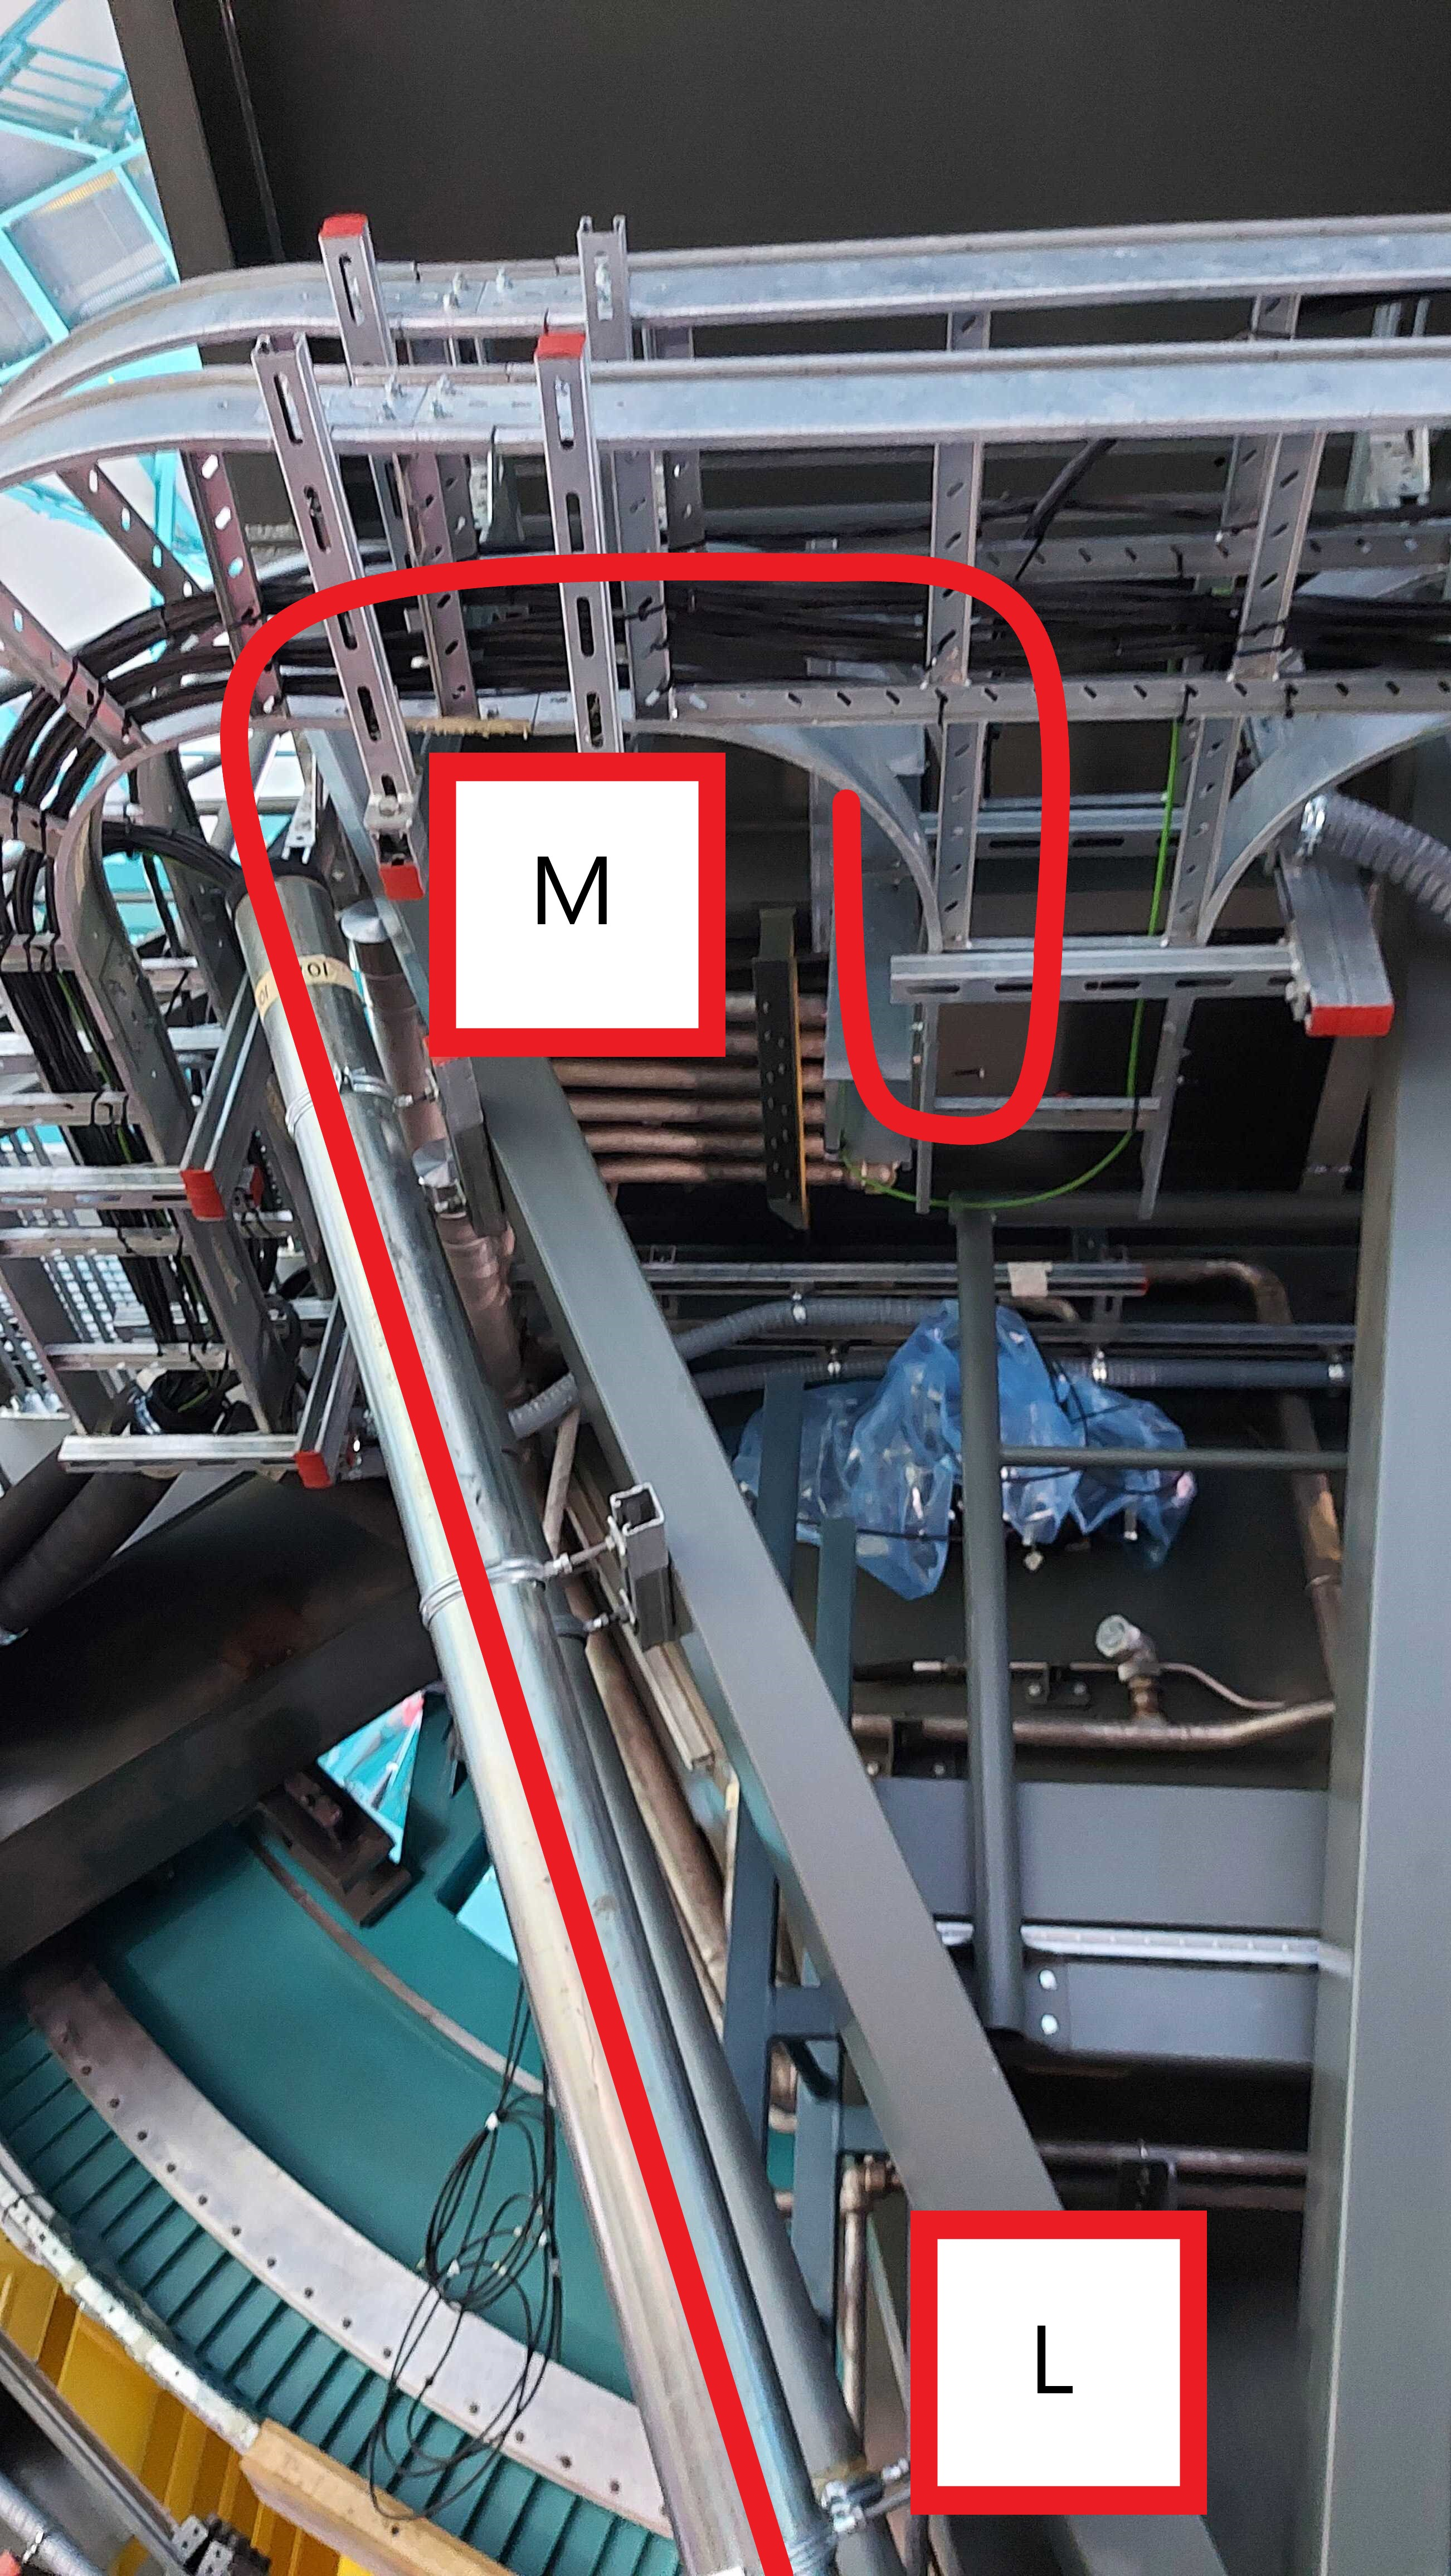
\includegraphics[width=\textwidth]{images/27-1.jpg}
    \end{subfigure}
    \caption*{From here point L shows up on the 8th floor at the base of the TMA, the cable is routed along with the cable tray and pipe found there to point M where the cable wrap is located.}
  \end{figure}

\newpage
  %Images
  \begin{figure}
    \centering
    \begin{subfigure}{0.45\textwidth}
      \centering
      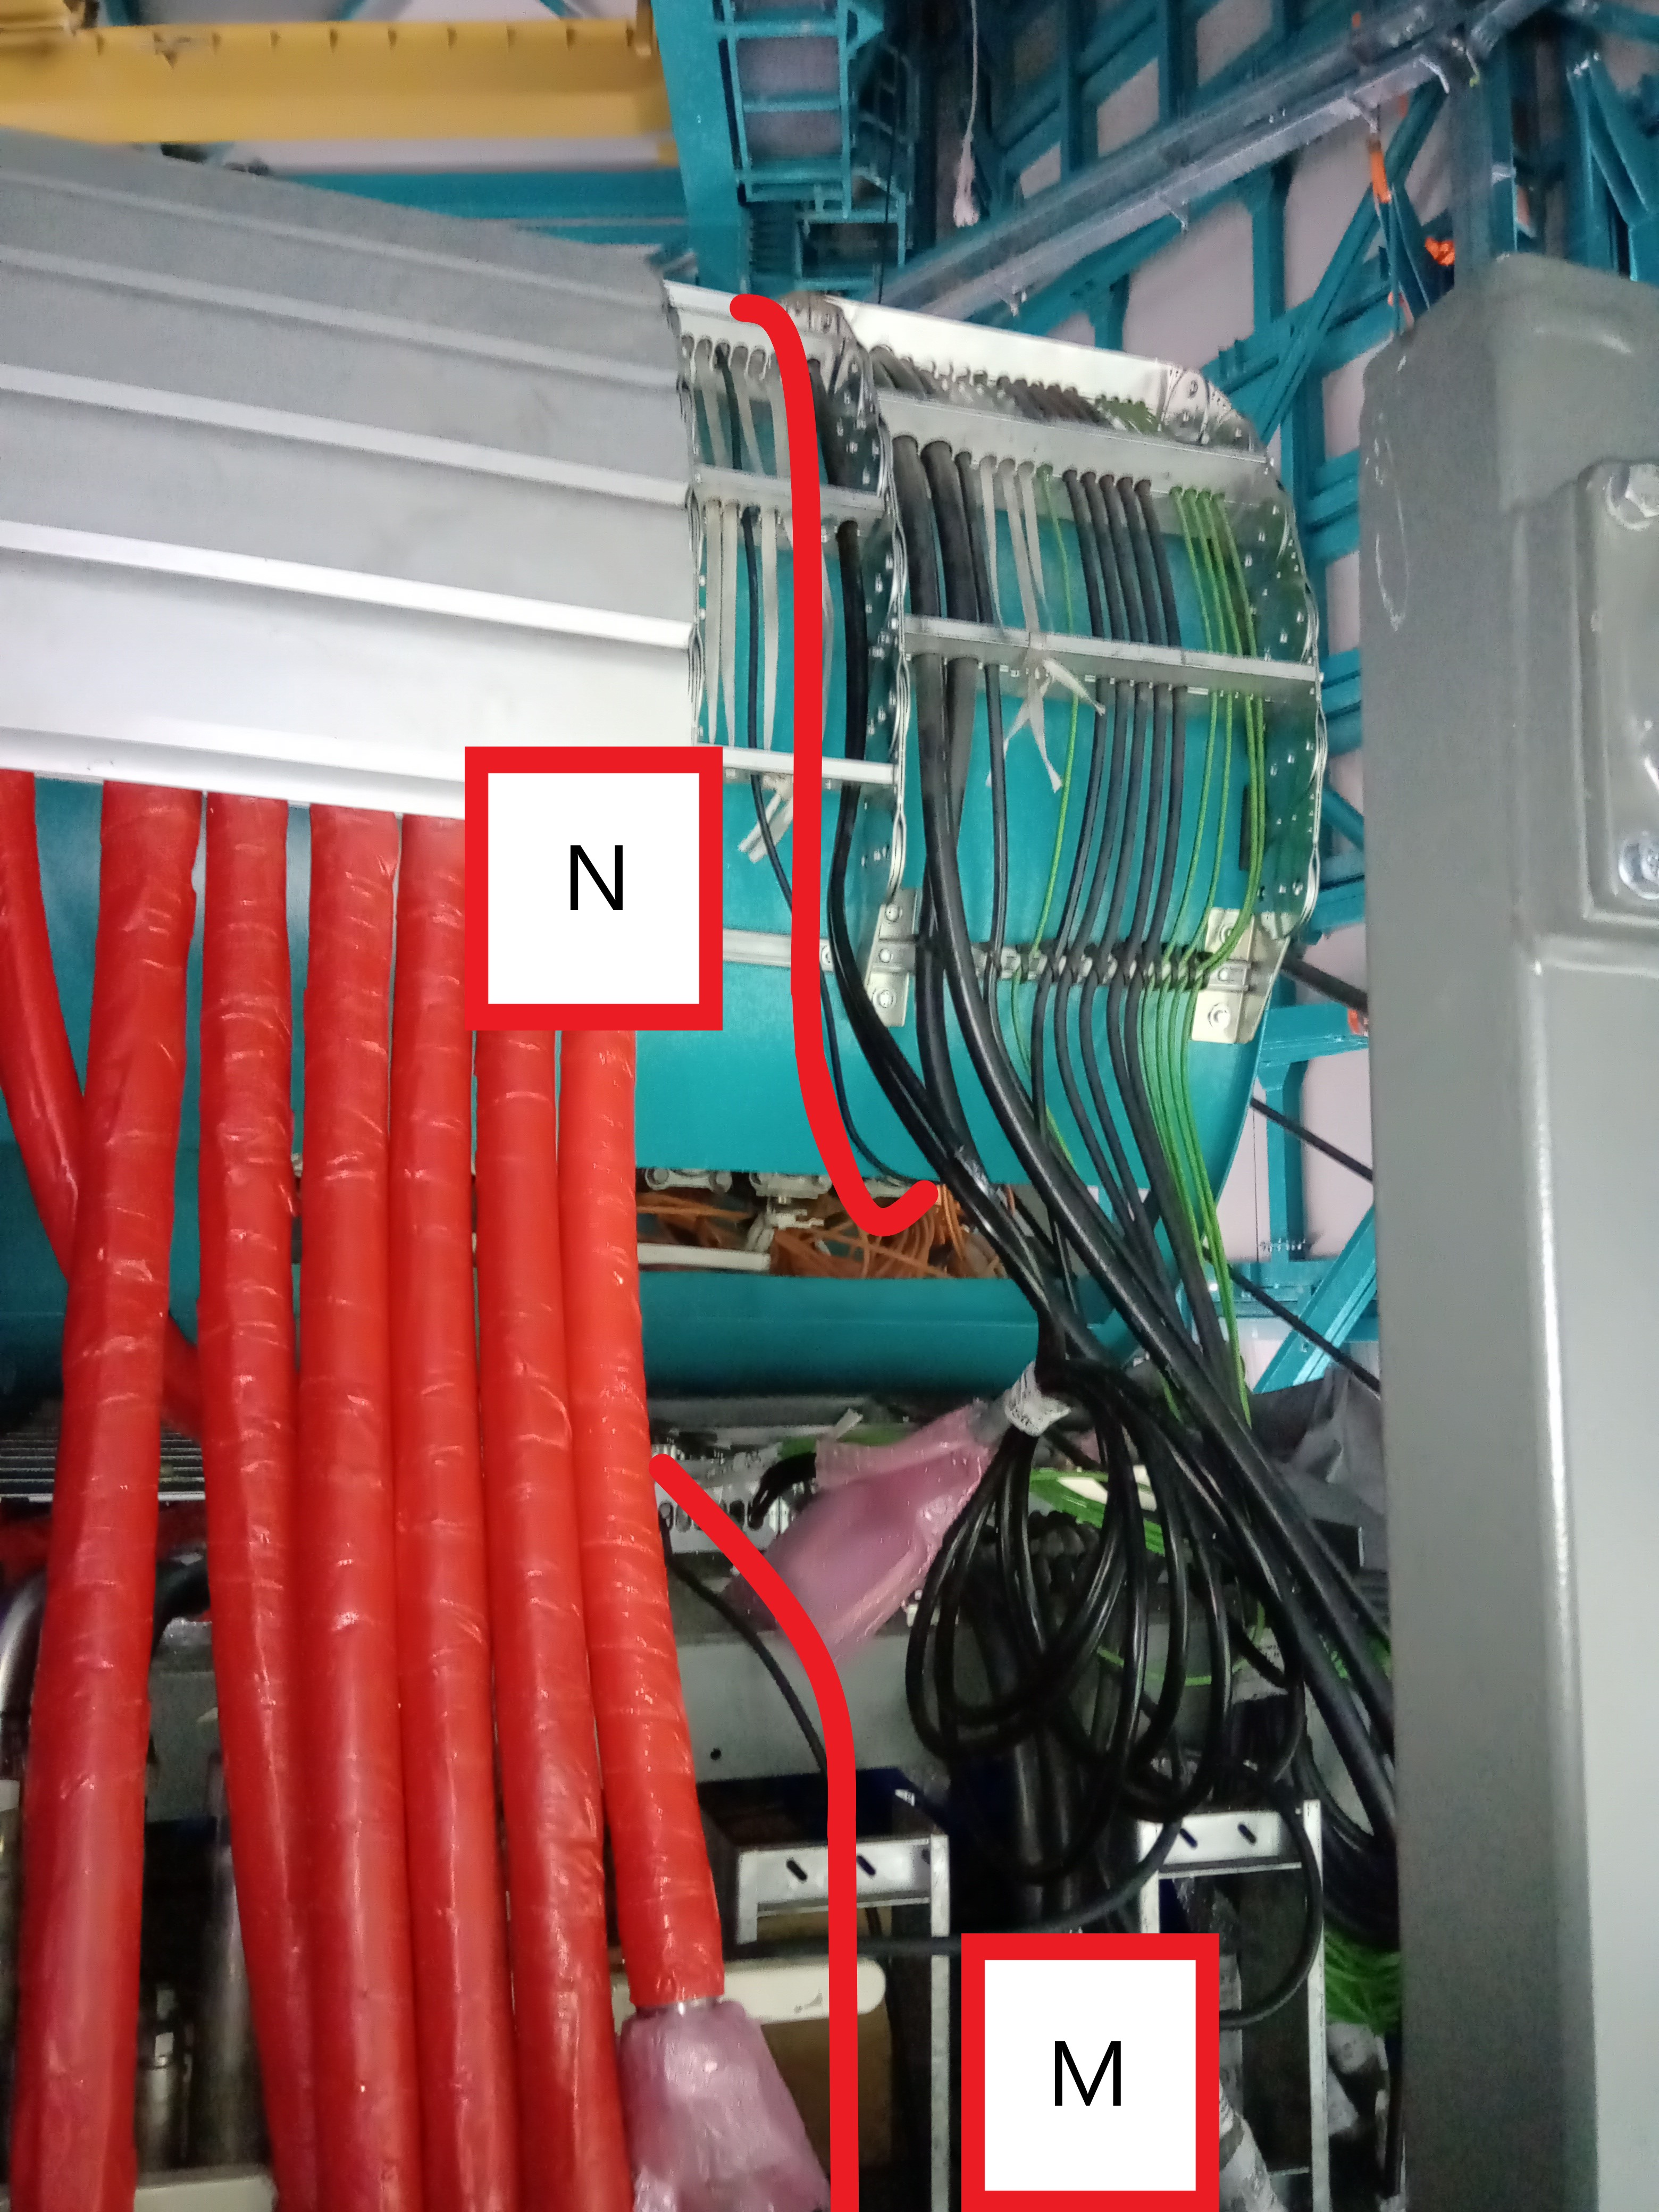
\includegraphics[width=\textwidth]{images/28.jpg}
      \caption*{From the base of the cable wrap CW on point M, the cable makes a full loop around it and connects from below to point N inside the cable wrap.}
    \end{subfigure}
    \hfill
    \begin{subfigure}{0.45\textwidth}
      \centering
      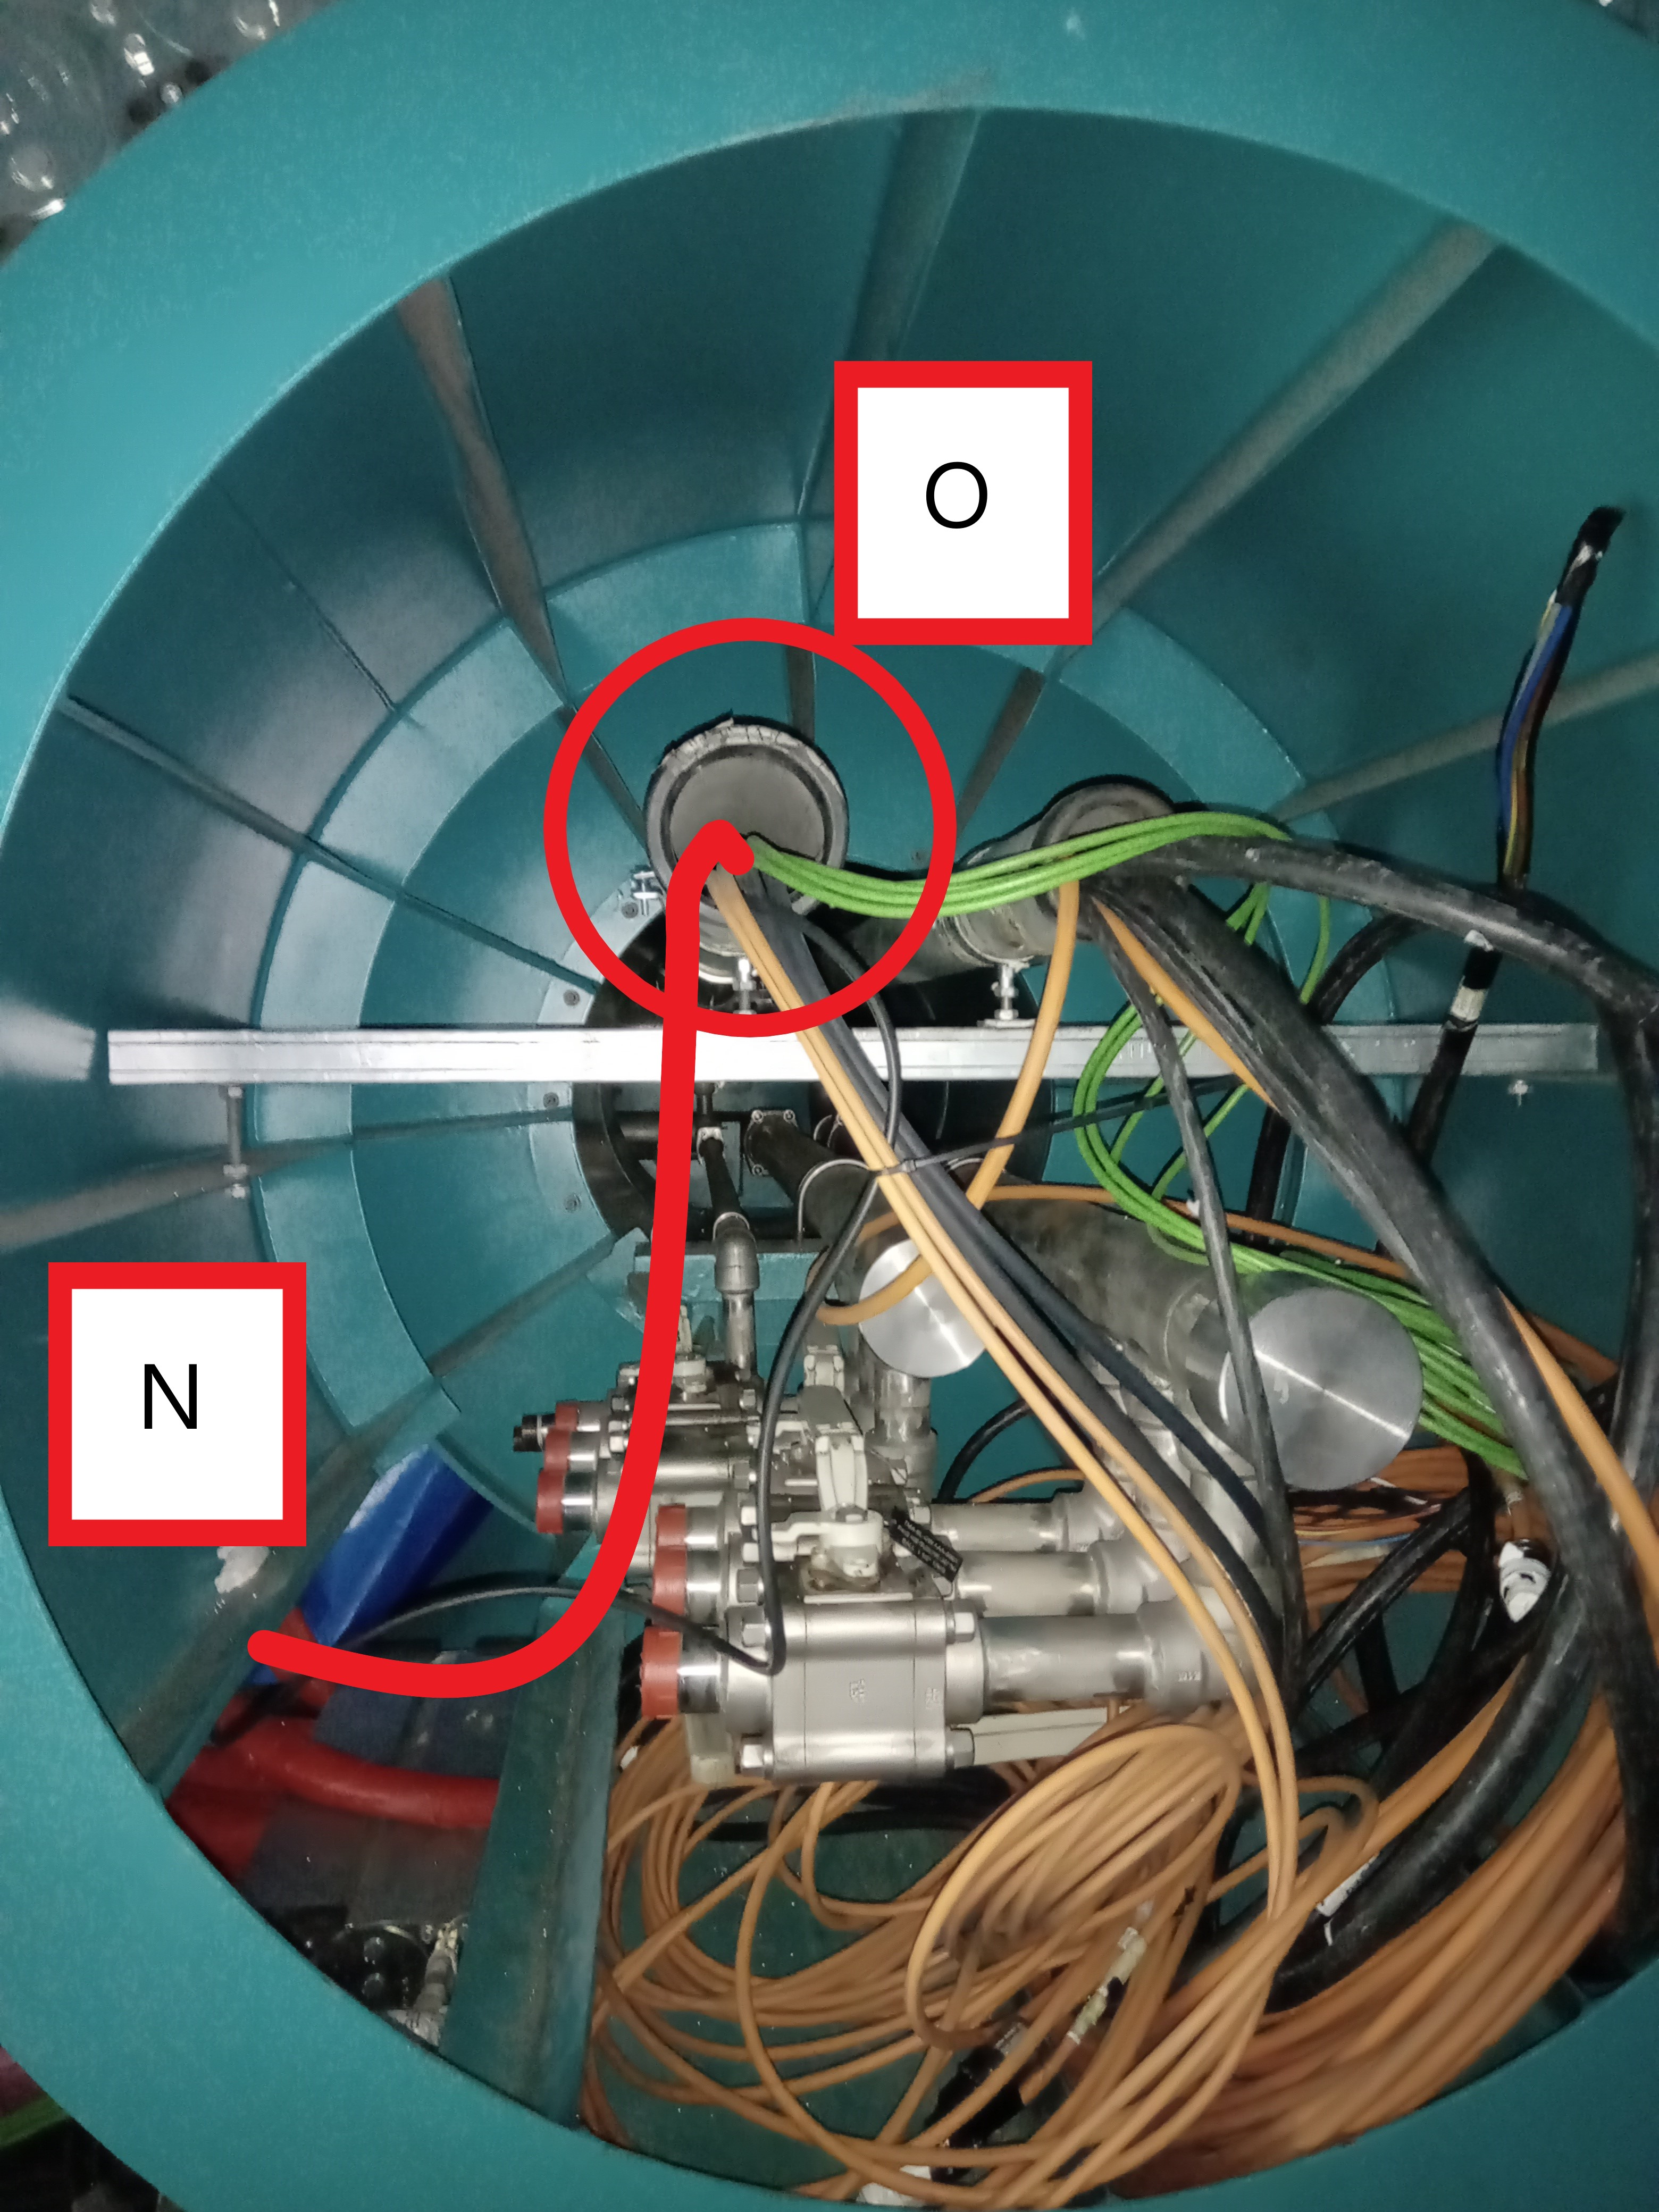
\includegraphics[width=\textwidth]{images/28-1.jpg}
      \caption*{The cable comes from under the cable wrap on point "N" and enters the tube located inside the CW  to position "O" and runs through the inside of the TMA structure to the top of the telescope.}
    \end{subfigure}
  \end{figure}

\newpage

\begin{figure}
  \centering
  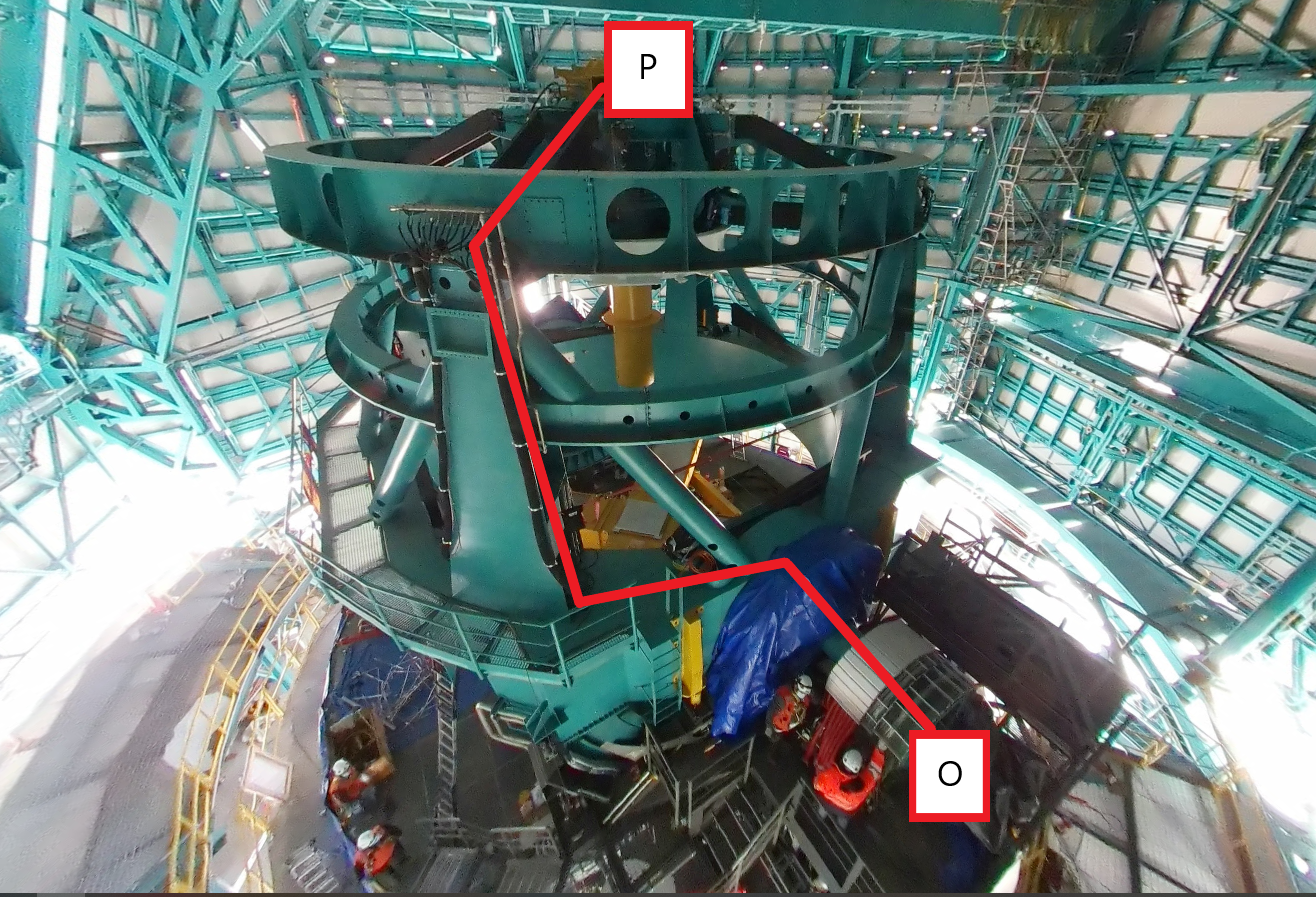
\includegraphics[width=20cm]{images/33.png}
  \caption*{The following image gives us a panoramic view of the cable route inside the TMA from point "O" to its final position at point "P" of the camera cable wrap CCW.}
\end{figure}

\newpage

\begin{figure}
  \centering
  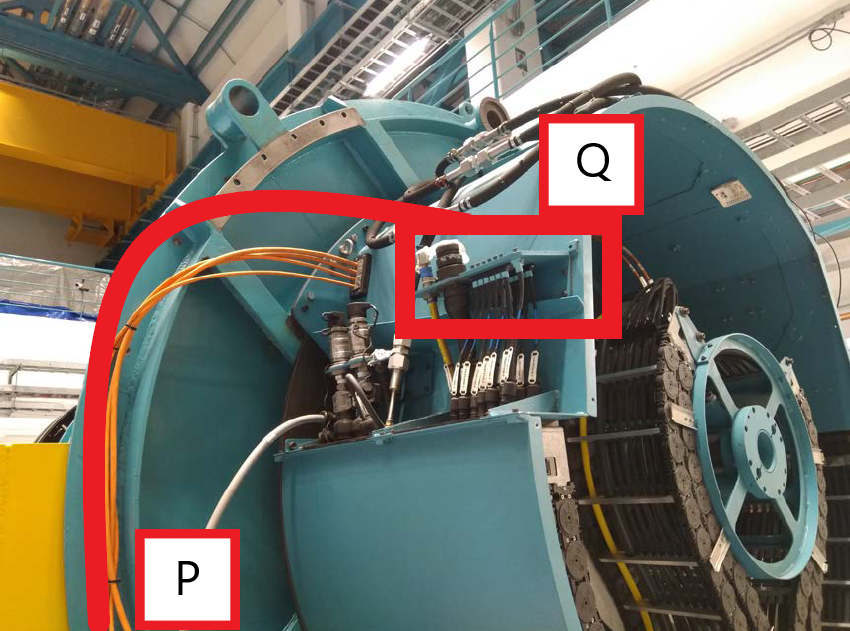
\includegraphics[width=20cm]{images/34.png}
  \caption*{From position "P" at the top of the telescope, the cable is routed along the spider connecting to position "Q" of the CCW as shown in the image.}
\end{figure}

\newpage

\section{Generalview of the fiber optic disconnection points}
\label{sec:disconnectpoints}
\vspace{30 mm}
\begin{figure}
  \centering
  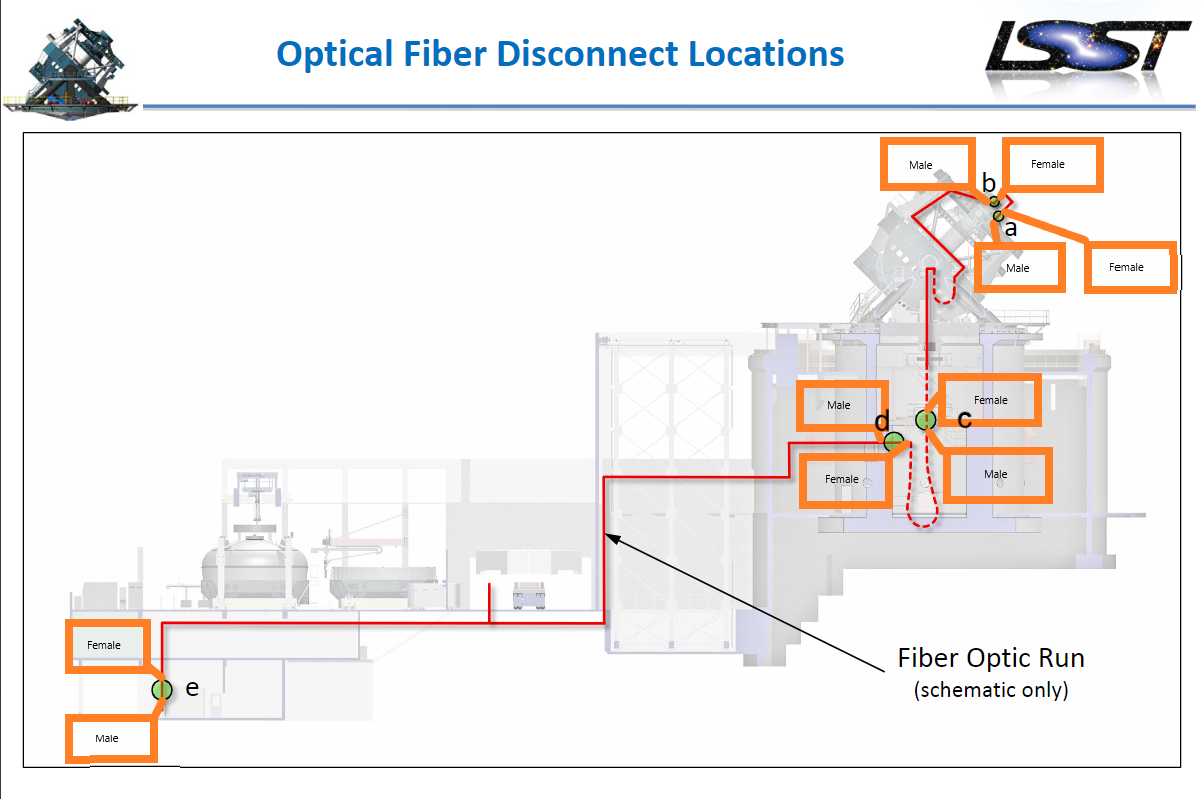
\includegraphics[width=17cm]{images/33333.png}
\end{figure}

\newpage

\section{Deployment Plan}

To carry out our implementation plan we will begin with the installation of a test fiber to obtain an exact measurement of the path of the MTP / MPO fiber that's going to be later installed in the future. The document \href{https://confluence.lsstcorp.org/display/IT/Network+Infrastructure+Low-Level+Design+LLD?preview=/139036736/140285500/Telescope-Camera%20Optical%20Fibers%20layout%20v3.pdf}{Network Infrastructure Low Level} provides us with an approximate measurement of the length of the cable that is going to be installed in which was calculated by a computerized program. Since this measurement was created by a computer and does not adjust to the real physical limitations that this project presents on the various segments of the cable. The IT Team opted to install this test fiber to get an exact measurement of the various segments where this cable will be routed.
The installation of this cable was carried out with a group force of 4 people in a period of 3 workdays for each segment that was installed. The next step is to purchase the 13 cables with the manufacturer along with 3 additional spares on a process that can take up to 2 months. Once we have these cables under our possession, the final installation period of all of these cables is expected to be around three months.

\newpage

  \subsection{Installation Timeframe}
  \begin{itemize}
    \item Before installing the cables, polarity tests will be performed in all of the cables to check that these have the correct gender polarity on a process that could take up to 2 days of work.  
  
    \item It will take approximately 9 days of actual work to install the 16 cables for segment 1 (point E to D), working at least 3 times a week. This segment requires the use of the Scissor lift machine. 
  
    \item It will take approximately 9 days of actual work to install the 13 cables for segment 2 (point D to C), working at least 3 times a week. This segment requires the use of the Scissor lift machine.
  
    \item It will take approximately 9 days of actual work to install the 13 cables for segment 3 (point C to B), working at least 3 times a week. This segment requires the use of the Man lift machine.
  
    \item Once installed, the final step is to inspect each one of these cables through a period of 3 days. 
  \end{itemize}
  Note: When installing these cables, we must pay close attention to the gender of the cable connector.

\newpage

  \subsection{Measurement Results}
  
  The measurements described below relate to the various points found in \hyperref[sec:disconnectpoints]{section 4} of this documentation.
  
  \begin{itemize}
    \item Segment E to D: The total lenght for segment E to D is 91mt.
    \item Segment D to C: The total lenght for segment D to C is 22mt.
    \item Segment C to B: The total length for segment C to B is 43mt.
  \end{itemize}
  The sum of all of these segments gives us a total length from point E to B of 156mt.
  \subsection{Deployment Conclusions and Considerations}
  \begin{itemize}
    \item We need at least 3 days to install and uninstall the test cable and to obtain a definitive measurement of the route.
    \item Wait around 2 months for the cables to be delivered and have them at the summit.
    \item Request any machinery or equipment necessary to carry out this task at least a week in advance with the managers in charge. 
    \item All cable installation work must be coordinated one week in advance.
    \item Consider at least 4 people to install the MTP / MPO cables in the future.
    \item It will take around 3 months to install these cables, working at least 3 times a week.
    \item When installing the cables, we have to pay close attention to the gender of the connector of the cable.
    \item The female connector will be located in the computer room and the male connector will be on the sixth floor.
  \end{itemize}

\newpage

  \subsection{Final Deployment}

The fibers were deployed as planned. 

Several fiber trays and pipes were installed to protect the fibers on its path, and a special metal structure was designed to be installed on the sixth-floor connection point. The objective of the design is to hold the fibers and prevent them from hanging on their weight, avoiding strain on the connection panel. Currently, the structure is sitill in construction phase, but its installation won't affect the fiber deployment. 

\label{sec:finaldeployment}
\vspace{10 mm}
\begin{figure}
  \centering
  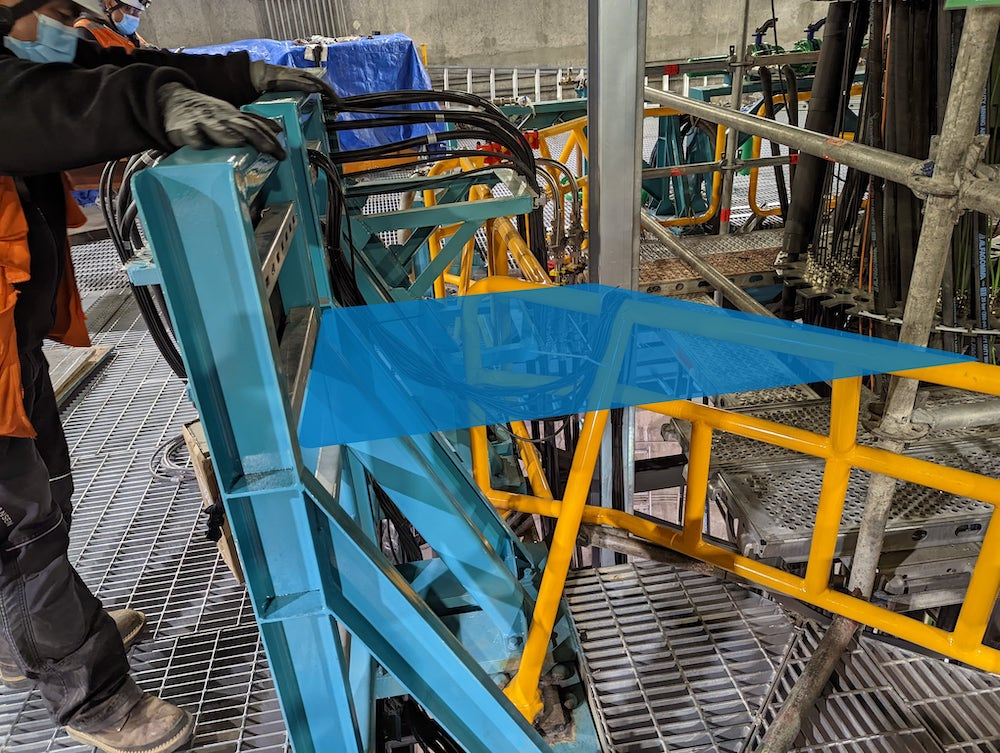
\includegraphics[width=11cm]{images/back_panel.jpg}
  \caption*{Concept design of back panel structure}
\end{figure}

Due to other work at the summit, the pandemic constraints, and the restrictions to access the TMA, the deployment of the fiber lasted more than expected. The actual work was accurate according to the plan but the execution had several interruptions increasing the time of each stage.
The certification of the fibers was the lengthiest stage, lasting approximately four months. The fibers were in place by December 2021, and were certified in March 2022.

\newpage

The 13 fibers were certified on each connection point, and light was injected using the DAQ on the computer room as the source. No data was sent using the fibers, but it is assumed that propagating light is sufficient proof of the functionality of the fibers. 

\vspace{5 mm}
\begin{figure}
  \centering
  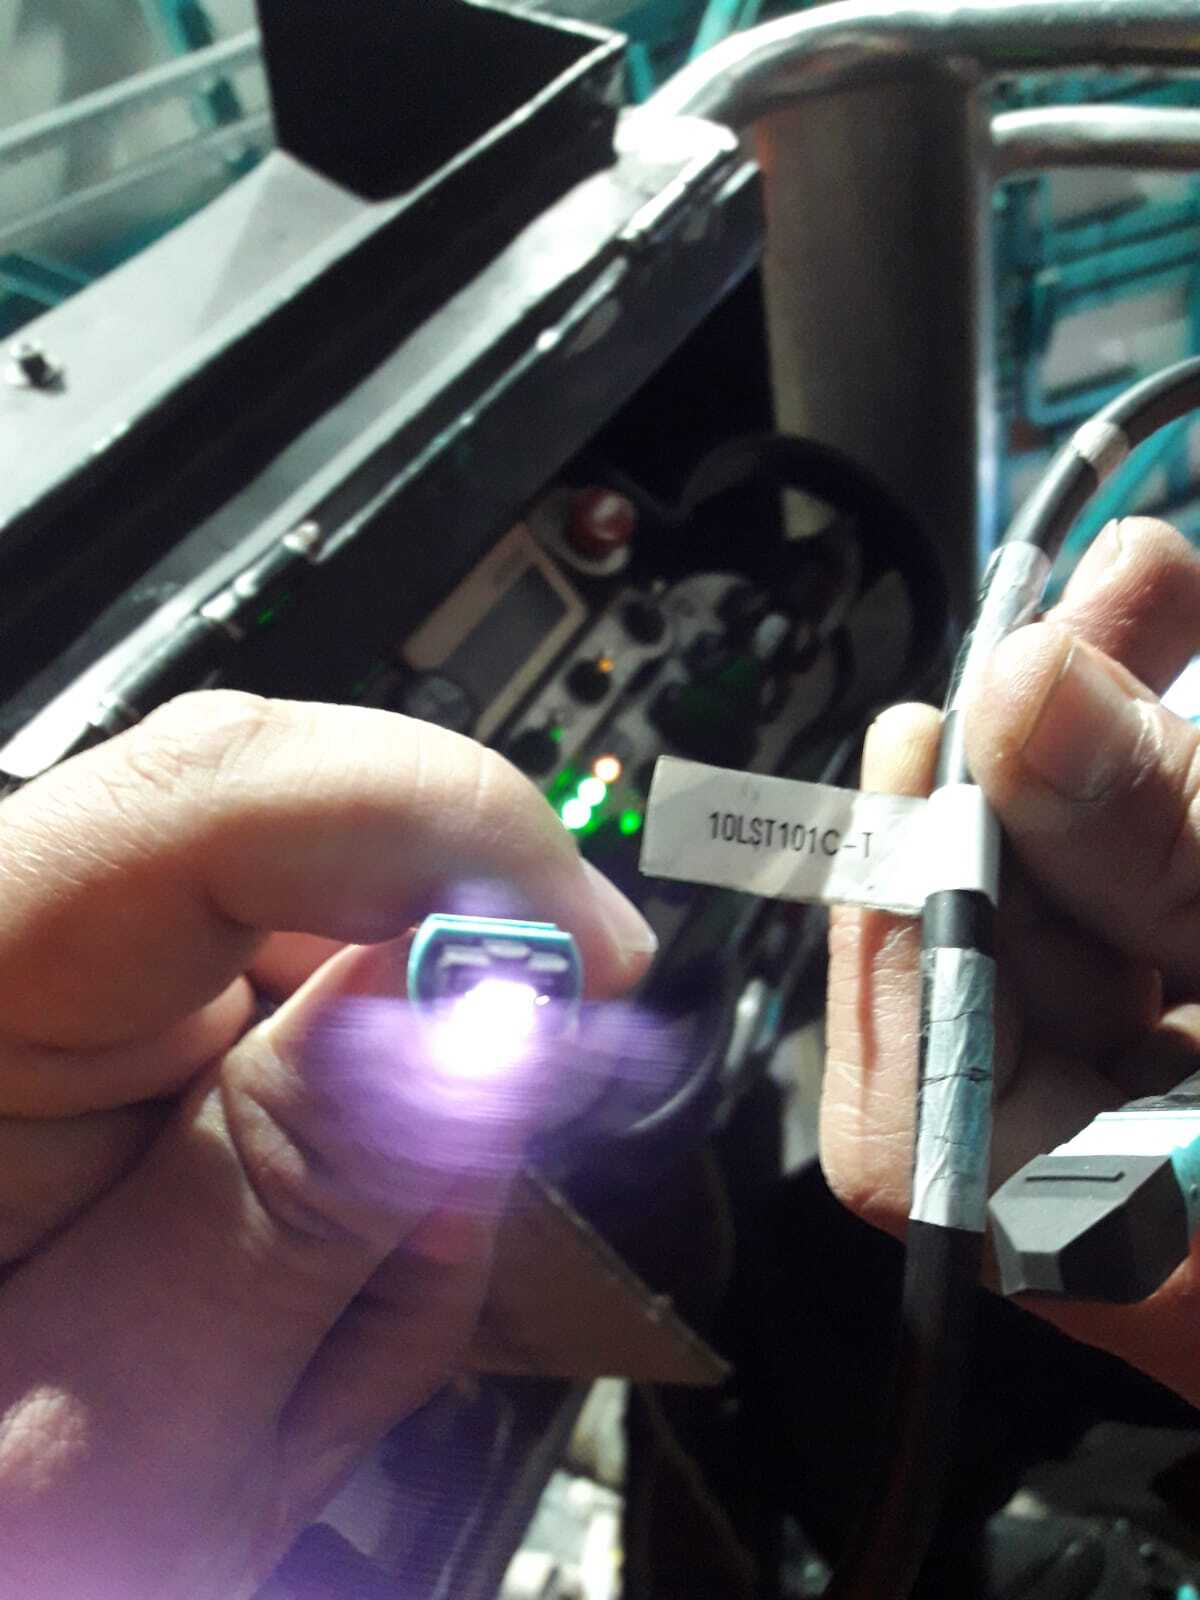
\includegraphics[width=8cm]{images/fiber_certification.jpg}
  \caption*{Image taken at the top of the TMA, sending light from the DAQ}
\end{figure}

\newpage










  









